\documentclass[upright, contnum]{umemoria}

%fix for the oneside argument
\makeatletter
\g@addto@macro\titlepage{\pagenumbering{Alph}}
\g@addto@macro\endtitlepage{\pagenumbering{roman}}
\makeatother

\depto{Departamento de Ingeniería Matemática}
\author{Reidmen Alexander Aróstica Barrera}
\title{}
\auspicio{PROYECTO FONDECYT 1151512}
\date{Noviembre 2018}
\guia{AXEL OSSES.}
\carrera{Magíster en Ciencias de la Ingeniería, Mención Matemáticas Aplicadas}
\memoria{Tesis para optar al Grado de \break
Magíster en Ciencias de la Ingeniería, Mención Matemáticas Aplicadas}
\comision{}

\usepackage{lipsum}

\usepackage[utf8]{inputenc}
\usepackage[T1]{fontenc}

\begin{document}

\frontmatter
\maketitle

\begin{abstract}
En el contexto del estudio biomecánico en medicina, hay diversas preguntas a ser respondidas fluctuando desde el modelamiento mismo de tejidos u organos a la simulación, predicción y validación de los diversos procedimientos experimentales para determinar factores clínicos de interés, tal como son los parámetros de espesor, porosidad, rigidez, etc. Este trabajo está orientado en esta dirección, mediante el cual se propone una formalización, justificación teorica y validación del problema directo de modelar el comportamiento mecánico de un hueso cortical de un nuevo procedimiento de ultrasonido. Asi, mediante la teoría de homogenización, se modela la propagación de una guia de ondas en un hueso poroso idealizado e implementa numericamente un modelo elastodinamico usando librerias al estado del arte. Los resultados obtenidos se comparan con la literatura reciente que propone el modelo experimental usado, validando el modelo numérico. Similarmente se estudia la presencia de viscosidad sobre el hueso mediante un modelo de Kelvin-Voigt, realizandose predicciónes al comportamiento viscoelastico del hueso, comparable con la literatura reciente. \\

In the context of biomechanical assessment of bone in medicine, there are abundant questions to be answer, fluctuating from the modelling itself of different tissues and organs to the simulation, prediction and validation of the different kind of experimental procedures to determine clinical factors of interest such as the thickness, porosity, stiffness constants, etc. This work is oriented in that direction in which its proposed a formalization, theoretical justification and validation of the direct problem associated to model the mechanical behavior on cortical bone from a novo ultrasound experimental procedure. By means of homogenization theory, its modelled the propagation of a guided-wave in porous bone and numerically implemented an elastodynamic model by applying state-of-art libraries using FEM method. The results obtained are the compared with the recent literature that propose the experimental procedure, thus validating the numerical model proposed. Similarly, its studied the presence of viscoelasticity type behavior in bone by applying a Kelvin-Voigt model, predicting the viselastic behavior, which in particular is comparable with recent and limited experimental literature.
\end{abstract}

\begin{dedicated}
A mi madre y padre, por todo.
\end{dedicated}

%\begin{thanks}
%\lipsum[1]
%\end{thanks}

\cleardoublepage

\tableofcontents
\listoftables % optional
\listoffigures % optional

\mainmatter

\begin{intro}
In the context of mechanical behavior in medicine, there are abundant question to answer, fluctuating from the mathematical modelling itself of different tissues, physiological structures, simulation of its experimental procedures to the verification and prediction of different factor of clinical interest such as density, stiffness constants, etc. From a computational modelling point-of-view, biological tissues define complex multiscale problems since there are multiple physical phenomena acting at various scales. Moreover, from the bast majority of clinical applications the materials are viewed in its continuous setting, thus the importance to contribute with mathematical models and numerical procedures to characterize non-trivial properties arising from the microscopic structures that affect the overall behavior in terms such as compressibility, elasticity or viscosity.
One of particular interest is the human bone, an absorbing complex composite structure that have an irregular hollow-like interior filled with marrow, surrounded by soft tissue and muscles. Over which it's defined the so-called bone quality, a composite of properties that enables bone to resist fracture. In this sense, when more bone is removed than added in the same time span, the so-called \textit{osteoporosis} condition appear, a established and well-defined disease from the World Health Organization, affecting more than 75 million of people in Europe, United States and Japan combined. being the major cause of fractures

Nowadays, noninvasive ultrasound techniques corresponds to a unique and important aspect in the biomedical research and applications, as they allow detailed insight of important bone parameters with a lower-cost, non-invasive and non-radiative properties that expects to challenge the gold-standard techniques used in clinical procedures. Under this setting, \textit{Minonzio et. al.} \cite{Minonzio2018} proposed a technique of wave-guide propagation to recover two relevant parameters that describe bone quality, the cortical and thickness of cortical bone, using an inverse-like problem formulation. Several questions must be addressed to successfully validate the technique, ranging from the study such as the underlying theory used, the effect of domain irregularities, robustness as well as the validation under controlled scenarios.

This work is oriented mainly in the modelling and numerical implementation of such novel ultrasound experimental procedure, in which via homogenization theory techniques it's studied the bone material mechanical behavior and their description using the \textit{Lamb}-curves theory, in which by means of a multiscale framework it incorporates the characteristic microstructure associated to the cortical bone, the so-called mesoscale. 
Over such a model is derived the cell problems that contains the relevant non-linearity of the two-scale asymptotic approximation being used, thus providing a methodology to verify and validate using simulated data and with respect to \textit{ex-vivo} results under controlled settings.

By using the two-scale homogenization framework, it's studied the macroscopic equations governing the composite bone material that incorporates the intrinsic non-linear microstructural behavior.
It gives us also an explicit step-wise algorithm that first computes the material homogeneous structucture and then describes the macroscopic \footnote{Depending on the literature being used, the macroscopic behavior is also expressed as effective or slow-variable behavior, since is the one that describes the nature defined typically on application fields as evolution problems, i.e. time dependent partial differential equation system.} model underlying the initial setting, allowing us an explicit formulation, thus implementation using the state-of-art \texttt{FEniCS} \cite{logg2012automated} library to compute the solutions of such kind of systems.

By implementing the ultrasound experimental procedure proposed from \textit{Minonzio, Foiret} \cite{Foiret2014}, \cite{Minonzio2018} its simulated  \textit{Lamb}-mode curves and singular values resembling the real behavior, assessing the parameter dependency and fidelity. In this context, it's studied properties of the elastic operator to account effects of resonance behavior in the frequency domain and instabilities observed in their spectral decomposition.
Similarly, numerically obtained homogenized elastic coefficients that model the effective mechanical behavior are compared with the reference literate, providing a standpoint towards further modification regarding symmetry, and domain configuration.
Finally, from a theoretical stand-point its studied the justification of the two-scale asymptotic expansion concluding on a convergence result, relating the multiscale solution of the composite material and the homogenized solution. Moreover the extension toward a viscoelasticity formulation regarding damping effects naturally appearing from the complex interaction between several tissues on the forearm.

\end{intro}
\chapter{Clinical Measurements}
\textit{Extracted from P\&G Paper, 2009} Cortical Bone is a highly organized hard and ligthweight tissue representing approximately 80\% of the skeletal mass in an human adult defined by an clear hiercharchy of microstructures. From a functional description, scaling down to nanometers its observed important structures for the cortical tissue such as Haversian Systems, Osteons, Lamellae, Collagen Fibres, Fibrils, and elementary mineral constituents with water. 

The standard description associated to a mechanical point of view is defining it as a two-phase composite material: a soft phase mainly of pores, containing organic fluid and soft tissues as cells, blood vessels, and a complex hard matrix phase with nerves distributed inside. Such a matrix consist mainly of hidroxyapatite and collagen. Porosity is distributed over various length scales, nevertheless only the two largest pores types: resorption cavities (with size of approx. $50-200 [\mu m]$ and Haversian canal (size of approx. $50 [ \mu m ]$ contribute to the so-called mesoscale structure thus the mechanical behavior of the cortical bone itself, hence the mesoscale porosity which is characteristic of the higher level of organization in bone. 

Computational modelling of biological tissues (in particular of bone) is a complex multiscale problem, since there are multiple physical phenomena interacting at various scales. Since in a bast majority of clinical applications the material are viewed as continuum, it's important to contribute in a mathematical model and numerical procedure to characterize non-trivial properties arising from the microscopic physical and geometrical structures affecting the overall behavior, in terms of effective compressibility (or viscosity) or elasticity. 

Nowadays, noninvasive resonance technique corresponds a unique and important aspect in the biomedical research and application, as the allow detailed insights of useful properties of bone such as porosity and thickness which corresponds to the primary steps necessary to the diagnosis of several diseases presented in adult human bone.

We'll study the cortical bone by the so-called asymptotic homogenization, which corresponds to a multi-scale method for determining the effective moduli of periodic media (\textit{Bakhvalov and Panasenko, 1989}). The approach exploits a separation of scales within the composite material, deriving an leading order homogenized equations governing the effective macroscopic behavior of the material.\\


\begin{figure}[!h]
	\centering
	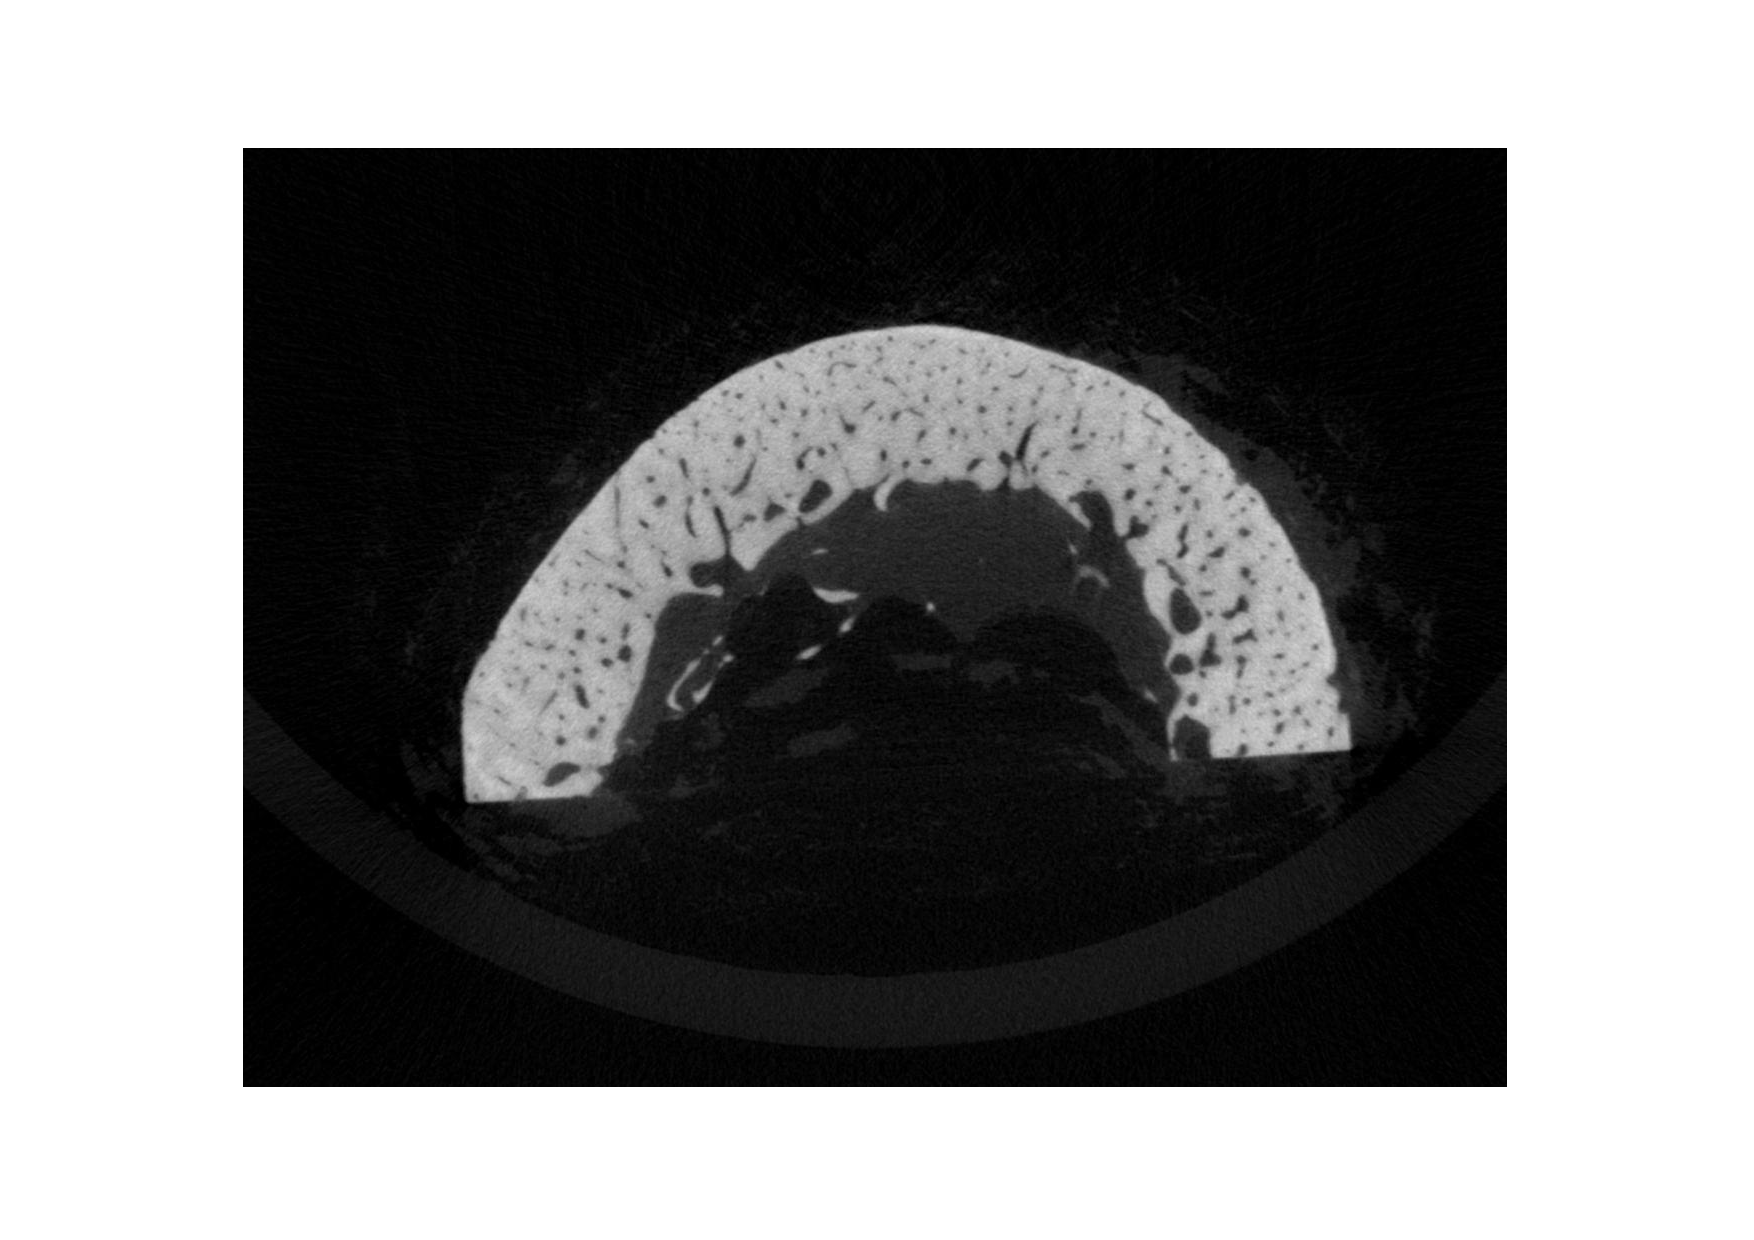
\includegraphics[scale=.5]{images/ImgExt/246-2010_rec0964.pdf}
	\caption{Real sample of $\mu$-CT image obtained, slice 246 of stack. \textit{France, 2010}.}
	\label{muCT-Image}
\end{figure}

\section{Time-domain Modelling}

Sophisticated quantitative ultrasound (QUS) approaches under study \cite{Foiret2014} \cite{Minonzio2018}, are based on the axial transmission measurements which consist of guided waves recordings that propagate into and through the cortex in response to an ultrasonic excitation produced at the surface and then studying their response in the form of dispersion curves \footnote{From a physical perspective, its represented as the variation of wave number $k = 2 \pi f/c(f)$ as function of the frequency $f \in [0, 2]$ being $c(f)$ the phase velocity of the mode.}, i.e., by means of the Lambs waves nonlinear equations \cite{Rhee2007},
Waveguide characteristics such as thickness and porosity can then be deduced from the dispersion curves by finding the best fitting of theoretical waveguide model to experimental data after a signal processing step. Such procedure define in particular the inverse problem under consideration.

In this section, its described the experimental procedure proposed by \cite{Minonzio2018} used to study two bone mechanical properties by means of a ultrasound transducer.
It is also given a brief explanation of the setting involved in the clinical procedure and the assumptions being done to model the recorded signal then processed by a spectrum technique. 

\subsection{Experimental Procedure}
The bone samples studies are subjected to the transmission of the wave-guide, i.e., a wave propagated from the external surface generated by a transducer device. 
Explicitly such force can be considered in the form:
\begin{equation*}
    \mathbf{F}(\mathbf{x},t) = A e^{-\frac{(t-t_0)^2}{2\sigma_0^2}} cos(2 \pi \tau_0 (t-t_0)) \text{ on } \Gamma_N
\end{equation*}
where $A > 0$ denotes an amplitude, $t_0 > 0$ a central time, $\tau_0$ some period and $\Gamma_N$ surface boundaries where the force is applied.
Even thought the shape of long segments of cortical bone is not uniform with respect to thickness nor in its surface, because of the device shape and size, it can be considered that such local spatial variations in the geometry are minimum and moreover can be neglected \cite{Foiret2014}. \\

As the transducer device captures the wave-guide over the long axis of bone, the propagation effects given on the axial (or anti-plane) of the wave does not add more relevant features in such a way that the natural 3-dimensional cylindrical-like shape of the bone can be simplified without affecting the overall behavior of interest to a 2-dimensional plate shape domain modelling the coronal cut plane of propagation. \\
%%%   
%%%
%%% CHECKED TO THIS POINT!
%%%   
%%%
For such a 2-dimensional wave-guide model, the propagation is studied by means of the homogenization technique in elastic and viscoelastic behaviors. Such a homogenization procedure results necessary since the size of microstructure generates restrictive computational costs, and moreover the ability of such theory to model the microstructure observed for example in (\ref{muCT-Image}), i.e., containing the porosity level implicitly in the elastic coefficients obtained by means of two-scale asymptotic framework.


\begin{figure}[!h]
	\centering
	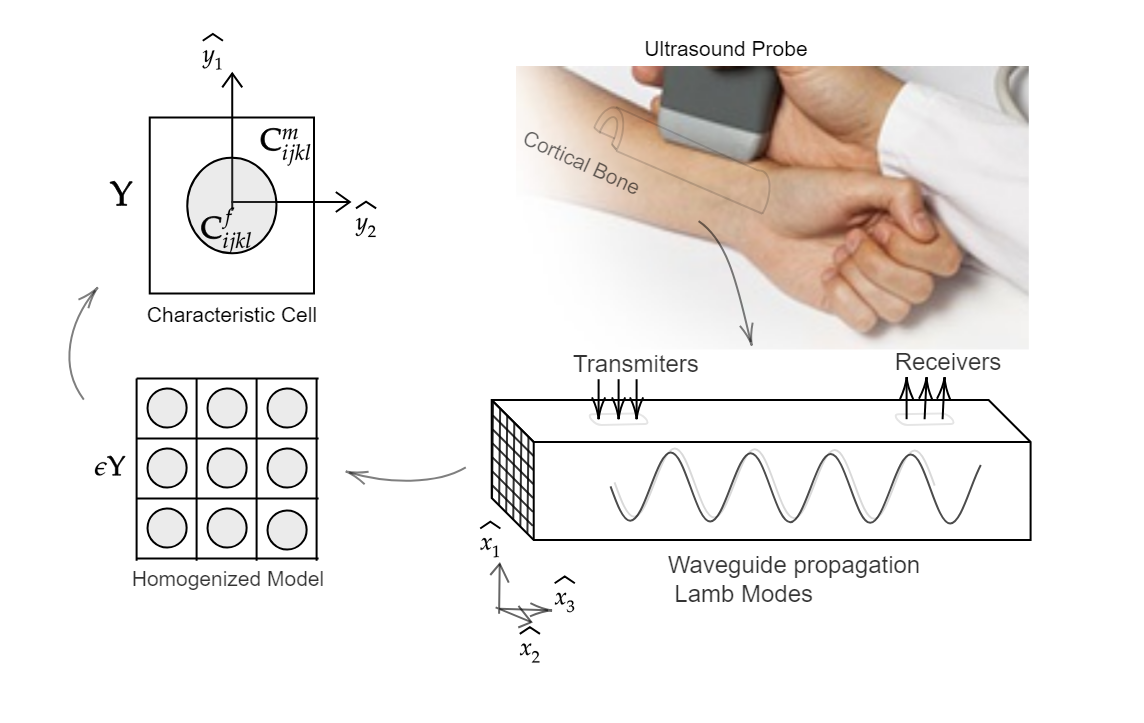
\includegraphics[width=0.7\textwidth]{images/ImgExt/SchematicPropagation.png}
	\caption{Schematic Procedure: from the experimental device to the homogenize idealization of the cortical bone.}
	\label{SchematicProp&Hom}
\end{figure} 

The important aspect for the transducer is the linear element array which contains several emitters and receiver. We model the experimental setting of the transducer applied on a patient as a elastodynamic model defined on the cortical bone, where we neglect the effects at the interface defined by the skin. 

In the case of simulations the number of emitters was fixed to 8 initially, but by the translation invariance of the elastic wave, the simulation only needed the emission using one emitter (or source), while the receptor where modeled by points in the surface containing the displacement vector.

\subsection{Signal Processing}
Each cycle of measurements consists of a sequential excitation of the $N^E > 0$ number of emitters located at boundaries $\Gamma_{e}$ as will be formalized later, which yield $N^E \times N^R$ time series arrays at each time of measurement.
Such a multi-channel series denoted by $\{ S(t_n, e_m,x_p) \}_{(n,p) \in [N^T]\times [N^R]}\}$ at fixed emitter $x_p, \, p \in \{1, \dots, N^E\}$ is then applied a 2-dimensional fast \textit{Fourier} transform obtaining $\{ \hat{S}(f_{\tilde{n}},e_m,k_{\tilde{p}}) \}_{(\tilde{n},\tilde{p}) \in [N^F]\times [N^K]}$\footnote{Which we identify following the literature of mechanics and ultrasound analysis as frequency and wavenumber respectively.}

Such Fourier transformed array $\hat{S}(\cdot, e_m, \cdot)$ for each emitter is then decomposed by singular values method (SVD), in the form:
\begin{equation*}
    P(e) \hat{D} P(e_m)^T = \hat{S}(e_m) \quad m \in \{1, \dots, N^E \}
\end{equation*}
which decomposed the spectral signal in its main singular values thus describing the relevant modes of mechanical behavior.
So, by applying the function over the first $N^E_*$ resonant modes defined by
\begin{equation*}
    L(P(e)) := \sum \limits_{e = 1}^{N^E_*} P(e) \overline{P(e)}
\end{equation*}
it describes the so-called \textit{Lamb} waves (or \textit{Lamb} branches) of propagation \footnote{Several studies consider the usage of this kind of curves, as ones mainly used to describe the material destruction and mechanical behavior, and moreover in a non-invasive form.} of the material \cite{Rhee2007}.

The inverse problem associated is then formulated as
\begin{equation*}
    (Th.^*, Po.^*) = \underset{(Th., Po.) \in \mathcal{A}}{\text{argmax}} \int\limits_{f_{min}}^{f_{max}} \frac{1}{M} \sum_{m=1}^M \left \vert \langle \hat{D}(k_m, f_p)\, \vert e^{ik_m(Th., Po., f_p} \rangle \right \vert
\end{equation*}
being $M>0$ the number of modes under to consider. Thus, the formulation is re-expressed as the recuperation of $(Th.^*, Po.^*)$, two revelant biomedical parameters describing the quality of cortical bone.

An important aspect of such \textit{Lamb} curves is the fact that implicitly contain the overall mechanical behavior of the elastodynamical model, so that define a useful tool for validation and comparison of numerical simulation with respect to real data. 


Over such a domain we consider their behaviour of linear elastodynamic type, defined by a displacement $u(\mathbf{x},t)$ with constitutive equation of linear (following \textit{Hookes} law), with forces $\mathbf{F}(t)$ applied at a section of the surface domain.

\section{Main assumptions and Multiscale Modelling}


Formally we consider the following:
Let a bounded domain $\Omega \subset \mathbb{R}^d$ ($d = 2,3$) represent the composed material under study, modelled by an incompressible, elastic matrix and several inclusion defining the so-called mesoscale being modeled mechanically by an elastic of cylindrical shape periodically distributed.
For the sake of the experimental setting under consideration, the exterior boundary $\partial \Omega$ is decomposed as
\begin{equation*}
	\partial \Omega = \Gamma_D \dot\cup \Gamma_N
\end{equation*}
denoting $\Gamma_D, \Gamma_N$ the Dirichlet and Neumann part of the exterior boundary respectively.

Furthermore, let the small parameter $0 < \epsilon \ll 1$ denote the aspect ratio between the macroscopic variable $\mathbf{x} \in \Omega$ and the microscopic one $\mathbf{y}$ in the form: $\mathbf{y} = \frac{\mathbf{x}}{\epsilon}$ being $\mathbf{y} \in \mathbf{Y}$ and $\mathbf{Y} = (0,1)^d$ the cell structure. In this configuration, the unitary cell $\mathbf{Y}$, can be decomposed as
\begin{equation*}
	\mathbf{Y} = \mathbf{Y}_m \cup \Gamma \cup \mathbf{Y}_p 
\end{equation*}
where $\mathbf{Y}_m$ and $\mathbf{Y}_p$ are defined as the domains occupied by the matrix and porous part respectively, and $\Gamma$ denotes the interface between them\footnote{This model is inspired in the development of the Homogenization of the elastic operator in a porous media proposed on \cite{christensen1982theory}. Nevertheless, this kind of configurations are typical in the two-scale homogenization literature \cite{panasenko2005multi-scale}, \cite{Boughammoura2013} to mention updated references.}.

Such a cell is assumed to be periodically distributed along the material, defining its highly oscillatory structure, suitable to use the the Homogenization framework. We consider the composite material of study with elastic properties having oscillation rate $\epsilon$, represented in the domain decomposition:
\begin{equation*}
	\overline{\Omega} = (\overline{\Omega}\setminus \Omega_1^{\epsilon}) \cup \overline{\Omega}^{\epsilon}_1
\end{equation*}
where we have defined
\begin{equation*}
    \overline{\Omega}^{\epsilon}_1 = \bigcup_{\mathbf{x} \in \mathbf{T}_{\epsilon}} \epsilon ( \mathbf{x} + \mathbf{Y} )
\end{equation*}
being the tessellation $\mathbf{T}_{\epsilon}$ the subset in $\mathbb{Z}^d$ of all points satisfying the conditions
\begin{equation*}
    \epsilon (\mathbf{x} + \mathbf{Y}) \subset \Omega, \quad \rho(\epsilon(\mathbf{x}+\mathbf{Y}), \partial \Omega) \geq \epsilon
\end{equation*}

Let us note in particular that for fixed $\epsilon >0$ and all $\mathbf{x} \in \Omega$ we have a unique decomposition $\mathbf{x}/\epsilon = \mathbf{x}_{\mathbf{T}_{\epsilon}(\mathbf{x})} + \mathbf{y}$ where $\mathbf{x}_{\mathbf{T}_{\epsilon}(\mathbf{x})}$ denotes the element in $\Omega$ of the tessellation.

The above considerations let us define finally the material coefficients as second order rank tensors for component $i,j,k,l \in \{1,\dots, d\}$ in the form:
\begin{equation*}
    C_{ijll}(\frac{\mathbf{x}}{\epsilon}) = C_{ijkl}(\mathbf{y}) \quad \text{for } \frac{\mathbf{x}}{\epsilon} = \mathbf{x}_{\mathbf{T}_{\epsilon}(\mathbf{x})} + \mathbf{y}, \, \mathbf{x} \in \Omega_1^{\epsilon}
\end{equation*}
and being $C_{ijkl}(\frac{\mathbf{x}}{\epsilon}) = 0$ if $\mathbf{x} \in \overline{\Omega} \setminus \Omega_1^{\epsilon}$.

\begin{figure}[!h]
	\centering
	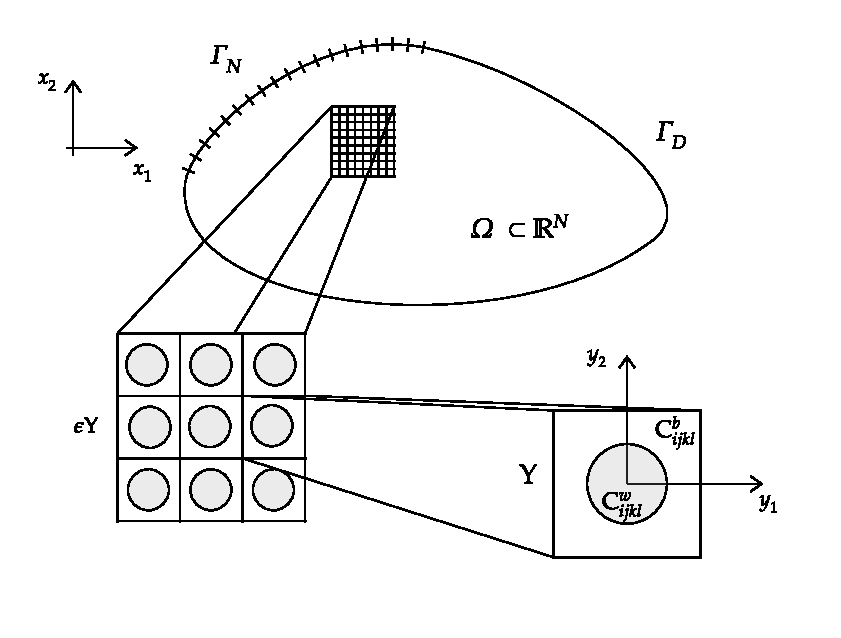
\includegraphics[scale=.8]{images/HomSchemes/HomBasicScheme.pdf}
	\caption{Homogenization Scheme of Bone: A composite periodic material at the long direction.}
	\label{HomBasicScheme}
\end{figure}

\begin{rem}
We model the material confined within the inclusion as a elastic (emulating a mechanical behavior of blood mixture mainly made of saturated static fluid) with volume $\epsilon^d \vert \mathbf{Y}_p \vert$ embedded in a elastic material (modeled mainly of hydroxipatite and collagen) filling a unit cell of volume $\epsilon^d \vert \mathbf{Y} \vert$.
We define, after scaling, the porosity associated to the material as the fraction of volume occupied by the gas in the unitary cell, i.e., 
\begin{equation*}
\phi = \frac{\vert \mathbf{Y}_p \vert}{\vert \mathbf{Y} \vert} = \vert \mathbf{Y}_p \vert
\end{equation*}
which will define the material coefficients dependent of such parameters.
\end{rem}

We denote the displacement $u(\mathbf{x},t) \in H^1(\Omega)$ with behaviour of linear elastic type subjected to surface forces $\mathbf{F}(t) \in L^2 (0, T)$, i.e., the material obeys the following initial boundary value problem:

\begin{equation*}
    \left \{
    \begin{aligned}
        \rho (\mathbf{x}) \partial_{tt} u(\mathbf{x},t) - \nabla \cdot \sigma (u) & = \mathbf{0}, \text{ in } \Omega \times (0, T) \\
        \sigma(u(\mathbf{x},t))_{ij} = \mathbf{C}_{ijkl} \mathbf{e}_{kl}(u(\mathbf{x},t)) & \text{ in } \Omega \times (0, T) \\
        u(\mathbf{x},t) = \mathbf{0} & \text{ on } \Gamma_D \times (0, T) \\
    \sigma(u(\mathbf{x},t)) \cdot n = \mathbf{F}(t) & \text{ on } \Gamma_N \times (0,T)
    \end{aligned}
    \right .
\end{equation*}

where $\mathbf{C}(\mathbf{x})$ denotes the elasticity tensor and $\mathbf{e}(u(\mathbf{x},t)) = \frac{1}{2}\big( \nabla u(\mathbf{x},t) + \nabla u(\mathbf{x},t)^{T}$ denotes the symmetric gradient.



\chapter{Homogenization and Justification}

Mechanical models of highly periodic structures within the asymptotic homogenization theory, which defines a multi-scale method for determining the effective moduli of periodic media, has been studied profoundly for example by \textit{Bakhvalov, Panasenko} \cite{bakhvalov1989homogenisation:}. The approach exploits a separation of scales within the composite material, deriving a leading order homogenized equations governing the effective macroscopic behavior of the material.\\

Given the assumptions for the multiscale elastodynamic model of cortical bone, the objective in this section will be to rigorously give a justification of the existence of such multiscale PDE system motivated from \cite{altenbach2018generalized}, then show the schematic procedure to obtain the so-called macroscopic mechanical behavior of bone (which is clear and keeps the mechanical behavior explicitly in the formulation with respect to other literature \cite{Parnell2008}) which will be used for the numerical simulations and finally give a convergence result of the solution between the multiscale model and the homogenized one. 

First, let us define the adequate spaces for our problem. Given the domain $\Omega \subset \mathbb{R}^d$, it will be denoted by $\mathbf{L}^2(\Omega)$ the $d$-dimensional vector functions, being each component on $L^2(\Omega)$. Similarly, it's defined the space $\mathbf{H}^1(\Omega)$ of d-dimensional vector functions, where as before, each component belongs to $H^1(\Omega)$ defined as usual in the literature \cite{evans2010partial}. 
In particular, denoting the vector trace operator by $\gamma: \mathbf{H}^1(\Omega) \rightarrow \mathbf{L}^2(\partial \Omega)$, we can define the space:
\begin{equation*}
    \mathbf{H}^1(\Omega, \Gamma_D) = \big \{ v \in \mathbf{H}^1(\Omega) \, \vert \, \gamma (v) \vert_{\Gamma_D} = \mathbf{0} \big \}
\end{equation*}

Moreover, by applying the \textit{Rellich-Kondrachov} theorem, the embedding from $\mathbf{H}^1(\Omega, \Gamma_D)$ into $\mathbf{L}^2(\Omega)$ is compact \footnote{From a more abstract point of view, it is possible to define $\kappa: \mathbf{L}^2( \Omega) \longrightarrow \mathbf{H}^{-1/2}(\Gamma_D)$ being the trace operator, i.e., $\kappa (u) = u \vert_{\Gamma_D}$. Then define an adequate space of square integrable vector functions with homogeneous Dirichlet condition on $\Gamma_D$ by $\mathbf{L}^2(\Omega, \Gamma_D) := \kappa^{-1}\big( \{ \mathbf{0}\}\big)$. Note that the operator $\kappa$ defined is linear and continuous in the corresponding spaces, moreover, since $\{\mathbf{0}\}$ is a close subset, then $\mathbf{L}^2(\Omega, \Gamma_D)$ is a close subspace of $\mathbf{L}^2(\Omega)$.
In particular, $\mathbf{L}^2(\Omega, \Gamma_D)$ is separable, so that there exist a Hilbertian base associated.}.

Given $\epsilon > 0$, let us fix $p \in (0,1)$ and consider $(C_{ijkl})_{ijkl}:=\mathbf{C}(p) \in \text{ lin}\big(\textbf{Sym}^{n\times n})$, the space of linear operator on the $n\times n$ symmetric matrices space, being uniformly elliptic and bounded elasticity tensors. Also, denote by $\rho^{\epsilon}(\mathbf{x}) = \rho \big( \frac{\mathbf{x}}{\epsilon}\big)$ an uniformly bounded density, $C_{ijkl}^{\epsilon}(\mathbf{x}) = C_{ijkl}(\frac{\mathbf{x}}{\epsilon})$ and consider for fixed parameter $T > 0$ the following evolution PDE problem modelling the displacements:
\begin{equation}
    \label{MainPDE}
    \left \{
    \begin{array}{cc}
        \rho^{\epsilon} \partial_{tt} u^{\epsilon} - \nabla\cdot \sigma^{\epsilon}(u^{\epsilon})= \mathbf{0} & \text{ in } (0,T) \times \Omega \\
        \sigma^{\epsilon}_{ij}(u^{\epsilon}) = C_{ijkl}^{\epsilon} \mathbf{e}_{kl}(u^{\epsilon}) & \text{ in } (0,T)\times \Omega \\
        u^{\epsilon} = \mathbf{0} & \text{ on } (0,T) \times \Gamma_D \\
        \sigma^{\epsilon}_{ij} n_j = \mathbf{F} & \text{ on } (0,T) \times \Gamma_N \\
        \partial_t u^{\epsilon} = u^{\epsilon} = \mathbf{0} & \text{ on } \{t=0\} \times \Omega
    \end{array}
    \right.
\end{equation}
\begin{prop}
Assuming $0 < \rho_0 \leq \rho\big( \frac{\mathbf{x}}{\epsilon} \big) < + \infty$ and $\mathbf{F} \in L^{\infty}(0,T;\mathbf{L}^2(\Omega,\Gamma_N))$, there exist a unique solution $u^{\epsilon}$ to (\ref{MainPDE}) for each $\epsilon > 0$, such that
\begin{equation*}
    u^{\epsilon} \in \mathcal{C}^0(0,T;\mathbf{H}^1(\Omega,\Gamma_D)) \cap \mathcal{C}^1(0,T;\mathbf{L}^2(\Omega))
\end{equation*}
\end{prop}

\begin{rem}
\footnote{The formulation of the elastodynamic problem with Dirichlet boundary conditions had been studied in various literatures, in particular on the multiscale works from \cite{panasenko2005multi-scale}, \cite{bakhvalov1989homogenisation:}. On the other hand, the formal study of Neumann boundary conditions has been done mainly on \cite{oleinik1992mathematical}.} In the following, inspired from \cite{raviart1983introduction}, a constructive proof is given based in the spectral decomposition of the elastic operator on $\mathbf{H}^1(\Omega, \Gamma_D)$ and solutions of the reduced ODE's associated to each eigenvalue. % of the elastic operator.
\end{rem}


Let us first note that problem (\ref{MainPDE}) can be rewritten in a variational form, satisfied in distributions over $(0,T)$ by: 
\begin{equation}
    \label{MainTimePDE}
    \begin{array}{cc}
        \text{Find } u^{\epsilon} \in \mathcal{C}^0 (0,T;\mathbf{H}^1(\Omega,\Gamma_D)) \cap \mathcal{C}^1(0,T;\mathbf{L}^2(\Omega)) & \text{ s.t. }\\
        \partial_{tt} (u^{\epsilon}(t),v)_{\Omega} + \mathcal{I}_{C}(u^{\epsilon}(t),v) = (\mathbf{F}(t),v)_{\Gamma_N}&  \forall v \in \mathbf{H}^1(\Omega,\Gamma_D) \\
        \partial_{t} u^{\epsilon}(0) = u^{\epsilon}(0) = \mathbf{0} & \\
    \end{array}
\end{equation}
being $\mathcal{I}_{C}(u,v) := \int_{\Omega} C_{ijkl}^{\epsilon}\mathbf{e}_{kl}(u^{\epsilon}(t)) \partial_{x_j} v_i$.
Let us prove the existence and uniqueness of solution for (\ref{MainTimePDE}).
\begin{proof}
\begin{enumerate}
    \item To this end, it will be considered approximate solutions to (\ref{MainTimePDE}). It is defined the subspace $V_m$ generated by the first $m \in \mathbb{N}$ eigenvectors $\{w_1, \dots, w_m \}$ being $(w_i)_{i \in \mathbb{N}} \subset \mathcal{C}^{\infty}(\Omega)$ a Hilbertian base of $\mathbf{H}^1(\Omega, \Gamma_D)$ were the regularity follows from bootstrap and by the Sobolev embedding.
    Then, let us consider the problem in time, defined by:
    \begin{equation}
        \label{ApproxTimePDE}
        \begin{array}{cc}
            \text{Find } u^{\epsilon}_m: t \in (0,T) \longrightarrow u_m(t) \in V_m & \text{ s.t. } \\
            \partial_{tt}(u_m^{\epsilon}(t),v)_{\Omega} + \mathcal{I}_{C}(u^{\epsilon}_m(t),v) = (\mathbf{F}(t),v)_{\Gamma_N} & \forall v \in \mathbf{H}^1(\Omega,\Gamma_D) \\
            \partial_{t} u^{\epsilon}_m(0) = u^{\epsilon}_m(0) = \mathbf{0} & \\
        \end{array}
    \end{equation}
    \begin{rem}
    Note that the linear operator $b(t)(v) := (\mathbf{F}(t),v)_{\Gamma_N}$ is well-defined and moreover continuous on $\mathbf{H}^1(\Omega,\Gamma_D)$ for each $t \in (0,T)$.
    This follows from the trace theorem applied on $\mathbf{H}^1(\Omega, \Gamma_D)$ since $\forall t \geq 0$, we have the bounds:
    \begin{align*}
        \vert b(t)(v) \vert & \leq \Vert \mathbf{F}(t) \mathbb{I}_{\Gamma_N} \Vert_{\mathbf{L}^2(\partial \Omega)} \Vert \gamma (v) \Vert_{\mathbf{L}^2(\Gamma_N)} \\
        & \leq \Vert \mathbf{F}\Vert_{\mathbf{L}^{\infty}(0,T;\mathbf{L}^2(\Gamma_N))} \Vert \gamma(v) \Vert_{\mathbf{L}^2(\partial \Omega)} \\
        & \leq \Vert \mathbf{F} \Vert_{\mathbf{L}^{\infty}(0,T;\mathbf{L}^2(\Gamma_N))} \Vert v \Vert_{\mathbf{H}^1(\Omega)}\\
        & = \Vert \mathbf{F}\Vert_{\mathbf{L}^{\infty}(0,T;\mathbf{L}^2(\Gamma_N))} \Vert v \Vert_{\mathbf{H}^1(\Omega, \Gamma_D)}
    \end{align*}
    \end{rem}
    Defining $u^{\epsilon}_m(t) = \sum_{i=1}^m \alpha_i^{\epsilon}(t) w_i$ with $\alpha_i^{\epsilon} (t) = (u^{\epsilon}_m(t),w_i)_{\Omega}$ it follows that the functions $\alpha_i^{\epsilon}$ are solutions to the ODE system:
    \begin{equation}
        \label{AlphaODE}
        \begin{array}{cc}
            \partial_{tt} \alpha_i^{\epsilon}(t) + \lambda_i \alpha_i^{\epsilon}(t) = (\mathbf{F}(t),w_i)_{\Gamma_N}& \forall t \in (0,T) \\
            \partial_t \alpha_i^{\epsilon}(0) = \alpha_i^{\epsilon}(0) = 0 & 
        \end{array}
    \end{equation}
    being $(\lambda_i)_{i \geq 1}$ a positive, increasing sequence of eigenvalues associated to the decomposition of the operator $\mathcal{I}_C(\cdot, \cdot)$.\\
    Let us note by applying the variation of parameters technique, that the solution to (\ref{AlphaODE}) is given in the form:
    \begin{equation}
        \label{AlphaODEsol}
        \alpha_i^{\epsilon} (t) = \frac{1}{\sqrt{\lambda_i}} \int\limits_0^t sin(\sqrt{\lambda_i} (t-s)) (\mathbf{F}(t),w_i)_{\Gamma_N} \, ds
    \end{equation}
    so that, defining the matrix for $\omega \in \mathbb{R}$ by:
    \begin{equation*}
        Q(\omega) =
        \begin{bmatrix}
        cos(\omega) & sin(\omega) \\
        -sin(\omega) & cos(\omega)
        \end{bmatrix}
    \end{equation*}
    it is obtained the following relation for the solution and their derivative in the form:
    \begin{equation}
        \label{MatrixODEsol}
        \begin{bmatrix}
        \sqrt{\lambda_i} \alpha_i^{\epsilon}(t) \\
        \partial_{t} \alpha_i^{\epsilon}(t) 
        \end{bmatrix}
        = \int \limits_0^t Q\big(\sqrt{\lambda_i}(t-s)\big)
        \begin{bmatrix}
        0 \\
        (\mathbf{F}(t),w_i)_{\Gamma_N}
        \end{bmatrix}
    \end{equation}
    
    \item Next, the sequence $(u^{\epsilon}_m)_{m \in \mathbb{N}}$ is of Cauchy type on the spaces $\mathcal{C}^0(0,T;\mathbf{H}^1(\Omega, \Gamma_D))$ and $\mathcal{C}^1(0,T; \mathbf{L}^2(\Omega))$.\\
    Let $m,p$ be two integers such that $p > m \geq 1$ then from (\ref{AlphaODEsol}) it follows that
    \begin{equation*}
        \mathcal{I}_C(u_p^{\epsilon}(t)- u_m^{\epsilon}(t),u_p^{\epsilon}(t)- u_m^{\epsilon}(t)) + \vert \partial_t (u_p^{\epsilon}(t)- u_m^{\epsilon}(t))_{\Omega} \vert^2 = \sum_{i=m+1}^p \big( \lambda_i \vert \alpha_i^{\epsilon}(t) \vert^2 + \vert \partial_t \alpha_i^{\epsilon}(t) \vert^2 \big) 
    \end{equation*}
    and since $Q(\omega)$ is an orthogonal matrix, from (\ref{MatrixODEsol}) it follows that
    \begin{equation}
        \label{AlphaBound}
        \big( \lambda_i \vert \alpha_i^{\epsilon}(t) \vert^2 + \vert \partial_t \alpha_i^{\epsilon}(t) \vert^2 \big)^{1/2} \leq \int \limits_0^t \vert (\mathbf{F}(t),w_i)_{\Gamma_N} \vert \, ds 
    \end{equation}
    so that, by using the Cauchy-Schwatz inequality, it can be obtained
    \begin{align*}
        \lambda_i \vert \alpha_i^{\epsilon}(t) \vert^2 + \vert \partial_t \alpha_i^{\epsilon}(t) \vert^2 &\leq 2 \big( \int_0^t \vert (\mathbf{F}(t),w_i)_{\Gamma_N} \vert \, ds \big)^2 \\
        & \leq  2 t \int_0^t \vert (\mathbf{F}(t),w_i)_{\Gamma_N} \vert^2 \, ds
    \end{align*}
    from which it can be deduced the bound
    \begin{equation*}
        \mathcal{I}_C \big(u_p^{\epsilon}(t) - u_m^{\epsilon}(t),u_p^{\epsilon}(t) - u_m^{\epsilon}(t) \big) + \vert \partial_t (u_p^{\epsilon}(t) - u_m^{\epsilon}(t)) \vert^2 \leq 2 \sum_{i=m+1}^p t \int_0^t \vert (\mathbf{F}(s),w_i)_{\Gamma_N} \vert^2 \, ds
    \end{equation*}
    Now, since $\mathbf{F} \in L^{\infty}(0,T;\mathbf{L}^2( \Gamma_N))$ it follows
    \begin{equation*}
        \underset{p,m \longrightarrow + \infty}{\text{lim}} \sum_{i=m+1}^p \big \{ T \int_0^T \vert (\mathbf{F}(s),w_i)_{\Gamma_N}\vert^2 \, ds \big \} = 0
    \end{equation*}
    and by using the uniform elliticity of the tensor $\mathbf{C}$, it can be concluded that $(u_m^{\epsilon}(t))_{m \in \mathbb{N}}$ is a Cauchy sequence on the spaces $\mathcal{C}^0(0,T; \mathbf{H}^1(\Omega, \Gamma_D))$ and $\mathcal{C}^1(0,T; \mathbf{L}^2(\Omega, \Gamma_D))$.
    
    
    \item Since the above spaces are complete, there exist $u^{\epsilon}(t)$ limit as $m \longrightarrow +\infty$ of $u^{\epsilon}_m(t)$ belonging to the spaces $\mathcal{C}^0(0,T; \mathbf{H}^1(\Omega, \Gamma_D))$ and $\mathcal{C}^1(0,T; \mathbf{L}^2(\Omega))$.\\
    Let us see that $u^{\epsilon}$ effectively solves the problem (\ref{MainPDE}). To do this, let $m \geq 1$, and consider $\psi \in \mathcal{D}(0,T)$, since $u_m(t)$ solves (\ref{AlphaODE}) then it follows that:
    \begin{equation*}
        \int_0^T (u_m^{\epsilon}(t),v)_{\Omega} \partial_{tt}\psi(t) + \int_0^T \mathcal{I}_C (u_m^{\epsilon}(t),v) \psi(t)  = \int_0^T (\mathbf{F}(t),v)_{\Gamma_N} \psi(t) 
    \end{equation*}
    so that, in the limit as $m \longrightarrow 0$, the solution $u^{\epsilon}(t)$ solves the problem
    \begin{equation*}
        \int_0^T (u^{\epsilon}(t),v)_{\Omega} \partial_{tt}\psi(t) + \int_0^T \mathcal{I}_C (u^{\epsilon}(t),v) \psi(t) = \int_0^T (\mathbf{F}(t),v)_{\Gamma_N}\psi(t) 
    \end{equation*}
    with $\partial_t u^{\epsilon}(0) = u^{\epsilon}(0) = 0$ and the desired results follows. Moreover, continuity with respect to boundary data is obtained, since from (\ref{AlphaBound}) the solution $u^{\epsilon}(t)$ in the limit satisfies the inequality 
    \begin{equation*}
        \big( \mathcal{I}_C(u^{\epsilon}(t), u^{\epsilon}(t))+ \vert \partial_t u^{\epsilon}(t) \vert^2 \big)^{1/2} \leq \int_0^T \vert \mathbf{F}(t) \Vert \, dt \leq \Vert \mathbf{F}\Vert_{L^{\infty}(0,T;\mathbf{L}^2(\Gamma_N)}
    \end{equation*}
    and by the uniform boundness of the tensor $C$, the following bound is obtained
    \begin{equation*}
        \Vert u^{\epsilon} \Vert_{L^{\infty}(0,T;\mathbf{H}^1(\Omega, \Gamma_D))}  + \Vert \partial_t u^{\epsilon} \Vert_{L^{\infty}(0,T;\mathbf{L}^2(\Omega))} \lesssim \Vert \mathbf{F}\Vert_{L^{\infty}(0,T; \mathbf{L}^2(\Gamma_N))}
    \end{equation*}
    Note in particular that the above bound is independent of $\epsilon > 0$ since there is no dependency on the right-hand side of the inequality, from which follows well-possedness for each multiscale elastic problem with parameters $\epsilon > 0$.
\end{enumerate}

\end{proof}

%%%%%
%%%%% THE ABOVE ADDED 21/10/2018
%%%%%

Now, the idea is to obtain a result of time regularity for the solution of the multiscale elastodynamic model. The motivation comes from \textit{Panasenko} works, who obtained such type of results in a general viscoelastic case with full \textit{Dirichlet} boundary conditions.

In this case, it will be to used a bootstrap type method to obtain the time-regularity for the mixed boundary problem, using the bounds derived from spectral theory.

\begin{prop}
\label{BootstrapingProp}
Let $u^{\epsilon} \in \mathcal{C}^{0}(0,T; \mathbf{H}^1(\Omega, \Gamma_D))$ denote the unique solution of the mixed boundary multiscale problem and suppose also the regularity for the parameters and surface force given by $A^{jk} \in L^{\infty}(\mathbf{Y})$ and $\mathbf{F} \in \mathcal{C}^p(0,T; \mathbf{L}^{2}(\Gamma_N))$, then for each $p \geq 1$ we have that:
\begin{equation*}
    u^{\epsilon}, \partial_t u^{\epsilon} \in \mathcal{C}^p(0,T; \mathbf{L}^2(\Omega))
\end{equation*}
\end{prop}
\begin{rem}
In particular, from the proof it's also possible to obtain that
\begin{equation*}
    u^{\epsilon}, \partial_t u^{\epsilon} \in \mathcal{C}^p(0,T; \mathbf{H}^1(\Omega, \Gamma_D))
\end{equation*}
\end{rem}

\begin{proof}
Let us develop the main idea of the proof:\\
\begin{enumerate}
    \item Using the spectral theory for the existence of multiscale problem, it is obtained a solution $u^{\epsilon}$ having regularity:
    \begin{equation*}
        u^{\epsilon} \in \mathcal{C}^0(0,T;\mathbf{H}^1(\Omega, \Gamma_D)) \cap \mathcal{C}^1(0,T;\mathbf{L}^2(\Omega))
    \end{equation*}
    thus the results being valid for initial cases $p = 0, 1$.
    \item Let us take $\vert h \vert \ll 1$ such that $t+h \in (0,T)$ and define the difference with parameter $\epsilon > 0$ fixed as:
    \begin{equation*}
        u_h^{\epsilon}(t, \mathbf{x}, \frac{\mathbf{x}}{\epsilon}) := u^{\epsilon} (t+h, \mathbf{x}, \frac{\mathbf{x}}{\epsilon}) - u^{\epsilon}(t, \mathbf{x}, \frac{\mathbf{x}}{\epsilon})
    \end{equation*}
    Now, defining the difference of surface forces as
    \begin{equation*}
        \mathbf{F}_h(t):= \mathbf{F}(t+h) - \mathbf{F}(t)
    \end{equation*}
    it follows that the problem satisfied for functions $u_h^{\epsilon}$ is given by:
    \begin{equation*}
        (P_{\epsilon}) \left \{
        \begin{array}{cc}
            \rho^{\epsilon} \partial_{tt} u_h^{\epsilon} - \partial_{x_j} \big( A^{jk}(\frac{\mathbf{x}}{\epsilon}) \partial_{x_k} u_h^{\epsilon} \big) = \mathbf{0}  &  \text{ in } (0,T)\times \Omega \\
            A^{jk}(\frac{\mathbf{x}}{\epsilon}) \partial_{x_k} u_h^{\epsilon}n_j = \mathbf{F}_h & \text{ on } (0,T)\times \Gamma_N \\
            u^{\epsilon}_h = \mathbf{0} & \text{ on }(0,T)\times \Gamma_D
        \end{array}
        \right .
    \end{equation*}
    with initial condition at rest (i.e. $\partial_t u_h^{\epsilon} = u_h^{\epsilon} = \mathbf{0}$ on $\{t=0\} \times \Omega$).
    
    
    \item Using the assumption of regularity for the surface force $\mathbf{F}$, let us recall from spectral theory the bound:
    \begin{equation*}
        \Vert u_h^{\epsilon} \Vert_{\mathbf{H}^1(\Omega, \Gamma_D)} + \Vert \partial_t u_h^{\epsilon}\Vert_{\mathbf{L}^2(\Omega)} \lesssim \int \limits_t^{t+h} \Vert \mathbf{F}(s) \Vert_{\mathbf{L}^2(\Gamma_N)} \, ds
    \end{equation*}
    so, from the continuity it is obtained that as $h \rightarrow 0$, the terms 
    \begin{equation*}
        \Vert u_h^{\epsilon} \Vert_{\mathbf{H}^1(\Omega, \Gamma_D)}, \Vert \partial_t u_h^{\epsilon} \Vert_{\mathbf{L}^2 (\Omega)} \rightarrow 0
    \end{equation*}
    then $u^{\epsilon} \in \mathcal{C}^2(0,T; \mathbf{L}^2(\Omega))$.
    
    
    \item Now, let us observe that we can take a time derivative to the full problem $(P_{\epsilon}$, and obtain a similar multiscale problem. Applying again the spectral theory, it is possible to obtain a solution $v_h^{\epsilon} = \partial_t u_h^{\epsilon}$, satisfying same bounds as before. In such a way, it follows that:
    \begin{equation*}
        \Vert \partial_{tt} u_h^{\epsilon} \Vert_{\mathbf{H}^1(\Omega, \Gamma_D)} + \Vert \partial_t u_h^{\epsilon} \Vert_{\mathbf{L}^2 (\Omega)} \lesssim \int_t^{t+h} \Vert \partial_t \mathbf{F}_h(t) \Vert_{\mathbf{L}^2(\Gamma_N)}
    \end{equation*}
    so that, as $h \rightarrow 0$ we conclude the regularity
    \begin{equation*}
        \partial_t u_h^{\epsilon} \in \mathcal{C}^0(0,T;\mathbf{H}^1(\Omega, \Gamma_D)) \cap \mathcal{C}^1(0,T;\mathbf{L}^2(\Omega)) 
    \end{equation*}
    then
    \begin{equation*}
        u_h^{\epsilon} \in \mathcal{C}^3(0,T; \mathbf{L}^2(\Omega))
    \end{equation*}
    and by a bootstrap type argument, the results follows for each $p \geq 1$.
\end{enumerate}

\end{proof}


%%%%%
%%%%% THE ABOVE ADDED 21/10/2018
%%%%%

\section{Homogenization Procedure}

 In this section, it is described the procedure to obtain the effective (or macroscopic) equation derived from the multiscale model (\ref{MainPDE}) by means of asymptotic approximation of the displacement $u^{\epsilon}(\mathbf{x},t)$ proposed by the two-scale homogenization theory\footnote{The notation is inspired from \cite{altenbach2018generalized} which keeps the mechanical behavior explicitly stated in all the derivation of the homogenized model, thus keeping its physical interpretation in the context of solid mechanics.}. This framework enables us to obtain an effective PDE model governing the overall macroscopic mechanical behavior that incorporates the highly oscillatory microstructure variation by means of cell problems. It provides moreover an algorithmic procedure suitable for numerical implementation.

To give jargon regarding homogenization literature, the variable $\mathbf{x}$ is defined as slow or global coordinate, while $\mathbf{y}$ denote the fast or local variable, related by $\mathbf{y} = \epsilon^{-1}\mathbf{x}$ as used before. In particular, the $\epsilon$ parameter represent the highly-oscillatory periodicity assumed on the material components described by the cell structure.
%With the region $\Omega \subset \mathbb{R}^d$ and boundaries $\partial \Omega = \Gamma_D \dot\cup \Gamma_N$, the general model to study using engineering notation is described for fixed time $t \in \mathbb{R}_+$ by:
%\begin{equation}
%    \label{VectorPDE-Elasticity}
%    \left \{ 
%    \begin{array}{cc}
%        \rho^{\epsilon}\partial_{tt} u^{\epsilon}(t,\mathbf{x}) - div \, \sigma(u^{\epsilon}(t,\mathbf{x})) = \mathbf{0} & \text{ in } \Omega \\
%        u^{\epsilon}(\mathbf{x}, t) = \mathbf{0} & \text{ on } \Gamma_D\\
%        \sigma(u(\mathbf{x},t)) \cdot n = \mathbf{F}(\mathbf{x},t) & \text{ on } \Gamma_N
%    \end{array}
%    \right .
%\end{equation}
%where it is associated also a initial condition in the form $u(\mathbf{x}, t) = 0 \text{ in } \Omega \times \{0\}$. For the constitutive law, it is assumed generalized linear \textit{Hookes} behavior, i.e.
%\begin{equation}
%    \label{ConstituteEq}
%    \sigma^{\epsilon}(u^{\epsilon}(\mathbf{x}, t)) = \mathbf{C}^{\epsilon}(\mathbf{x}) : \mathbf{e}(u(\mathbf{x},t))
%\end{equation}
%where $\mathbf{C}^{\epsilon}(\mathbf{x}) = (C_{ijkl}(\frac{\mathbf{x}}{\epsilon})$, and $\mathbf{e}(u(\mathbf{x},t)) = \mathbf{e}_{kl}(u(t, \mathbf{x}))$ denotes the second rank strain tensor. In particular, the strain relationship in given in the form
%\begin{equation}
%    \label{StrainEq}
%    \mathbf{e}_{kl} (u(\mathbf{x},t)) = \frac{1}{2}\big( \partial_{x_l} u_k(\mathbf{x},t) + \partial_{x_k} u_l (\mathbf{x},t) \big)
%\end{equation}
%Moreover, additional conditions are assumed:
%\begin{enumerate}
%    \item It is taken $\mathbf{x}$ as the global coordinate, while $\mathbf{y}$ a fast (or local) variable in the form $\mathbf{y} = \epsilon^{-1}\mathbf{x}$ where the parameter $\epsilon$ represents the highly-oscillatory periodicity of the cell structure.
%    \item The stress tensor $C_{ijkl}$ satisfies that $\mathbf{C}^{\epsilon} (\mathbf{x}) = \mathbf{C}(\mathbf{x}/\epsilon)$ being Y-periodic (related to the fast variable microstructure length).
%\end{enumerate}

%Within the time-domain formulation (\ref{VectorPDE-Elasticity}) our interest is related in study the elastic operator. 


\subsection{Two-Scale Asymptotic Homogenization}
It is assumed that the displacement solution for problem (\ref{MainPDE}) can be expressed as an expansion at different $\epsilon$ scales. Thus, the solution is found by an asymptotic expression at each time $t \in \mathbb{R}_+$ in the form:
\begin{equation*}
    \label{AsymptoticExpansion}
    u^{\epsilon}(t, \mathbf{x}) = \sum_{a=0}^{\infty} \epsilon^a u^{(a)}(t, \mathbf{x},\mathbf{y}) 
\end{equation*}
where the vector functions $u^{(a)}(\mathbf{x}, \cdot)$ are assumed Y-periodic for each $a>0$, since the microstructure is assumed periodically distributed, spanning the full domain $\Omega$. More explicitly, it is assumed throughout, regularity in the form:
\begin{equation*}
    u^{(a)}(t, \mathbf{x},\mathbf{y}) \in \mathbf{H}^1\big(\Omega; \, \mathbf{H}^1_{\#}(\mathbf{Y})\big) \quad \forall a \in \mathbb{N}
\end{equation*}
In what follows, it will be imposed several restrictions for the proposed solution (\ref{AsymptoticExpansion}) to effectively satisfy the problem (\ref{MainPDE}). In particular, the regularity assumption will naturally arise from the equalities satisfied for each $u^{(a)}$.

Since there is an explicit relation between the slow and fast variables, it is considered expressions of strain rate dependent on each one. Let us define for $\Phi \in \mathcal{C}^{\infty}(\Omega \times \mathbf{Y})$ the expressions related to the strain rate dependent on the variable:
\begin{equation*}
    \mathbf{e}_{kl,\alpha} (\Phi(\alpha)) = \frac{1}{2}(\partial_{\alpha_l} \Phi_k (\alpha) + \partial_{x_k} \Phi_l (\alpha)) \quad \forall \alpha \in \{\mathbf{x}, \mathbf{y}\}
\end{equation*}
thus, after applying such expression over the strain tensor $\mathbf{e}(\cdot)$ it satisfies the relation at components $k,l$ given in the form:
\begin{equation}
    \label{Multiscale-Strain}
    \mathbf{e}_{kl} ( u^{(a)}(\mathbf{x}, \frac{\mathbf{x}}{\epsilon})) = \mathbf{e}_{kl,x}( u^{(a)} (\mathbf{x},\mathbf{y})) + \epsilon^{-1} \mathbf{e}_{kl,y} (u^{(a)}(\mathbf{x},\mathbf{y}))
\end{equation}
%%%%%%%%%%%%
In the following, it is used a separation of scales to obtain the so-called homogenized coefficients, approximating the overall macroscopic (effective) behavior by applying the asymptotic approximation, i.e.,
\begin{equation*}
    \rho^{\epsilon}(\mathbf{x}) u(\mathbf{x}, \epsilon) + P^{(\epsilon)}(u(\mathbf{x},\epsilon) \sim \mathcal{O}(\epsilon^{\gamma}) \quad \gamma \geq 0
\end{equation*}
where the elasticity operator $P^{(\epsilon)}$ is expected to satisfy:
\begin{equation}
    \label{P-Operator}
    P^{(\epsilon)}(u(\mathbf{x},\epsilon) \sim - div \, (\mathbf{C}^{hom}(\mathbf{x}): \mathbf{e}(u^{(0)}(\mathbf{x}))) + \mathcal{O}(\epsilon)
\end{equation}
where $\mathbf{C}^{hom}(\mathbf{x})$ is some four-order tensor to be found and the right-hand side $\mathcal{O}(\epsilon^{\gamma})$ denotes the error expected from such an approximation. 

To handle derivatives from (\ref{P-Operator}), let us define the operator 
\begin{equation*}
    L_{\alpha \beta} (\cdot) = - \partial_{\alpha_j} \big( C_{ijkl} (\mathbf{y}) \mathbf{e}_{kl, \beta}(\cdot) \big), \quad \alpha, \beta \in \{ \mathbf{x},\mathbf{y} \}
\end{equation*}
And recall that, by the chain rule we have $\forall \, \Phi(\mathbf{x},\mathbf{y})$ enough regular vector function it follows:
\begin{equation*}
    \partial_{x_j} (\Phi (\mathbf{x}, \frac{\mathbf{x}}{\epsilon})) = \big \{ \partial_{x_j} \Phi (\mathbf{x}, \mathbf{y}) + \frac{1}{\epsilon} \partial_{y_j} \Phi(\mathbf{x},\mathbf{y}) \big \}_{\mathbf{y}= \epsilon^{-1}\mathbf{x}}
\end{equation*}

Now, using (\ref{AsymptoticExpansion}), the idea is to regroup in powers of $\epsilon$ thus impose constrains over each term $\epsilon^{(a)}$ to satisfy the main formulation (\ref{MainPDE}). To this end, note that from (\ref{P-Operator}) it follows:
\begin{equation*}
    P^{(\epsilon)}(u(\mathbf{x},\epsilon)) = A + B + C + \mathcal{O}(\epsilon)
\end{equation*}
where 
\begin{equation*}
    \begin{array}{cc}
        A &= P^{(\epsilon)}(u^{(0)}(\mathbf{x},\xi)) \\
        B &= \epsilon P^{(\epsilon)}(u^{(1)}(\mathbf{x},\epsilon)) \\
        C &= \epsilon^2 P^{(\epsilon)}(u^{(2)}(\mathbf{x},\epsilon)) \\
    \end{array}
\end{equation*}
Expanding every term, then using (\ref{Multiscale-Strain}), it follows:
\begin{align*}
    A &= - \partial_{x_j} \big( C_{ijkl}\mathbf{e}(u^{(0)}) \big) \\
    &=- \partial_{x_j} \big( C_{ijkl} \mathbf{e}_{kl,x} (u^{(0)}) + \frac{1}{\epsilon}C_{ijkl}\mathbf{e}_{kl,y}(u^{(0)} \big)\\
    &= - L_{xx}u^{(0)} - \frac{1}{\epsilon} L_{yx}u^{(0)} - \frac{1}{\epsilon} L_{xy}u^{(0)} - \frac{1}{\epsilon^2}L_{yy}u^{(0)}
\end{align*}
Similarly, for the other terms it can be obtained:
\begin{align*}
    B &= -\epsilon L_{xx} u^{(1)} - L_{yx}u^{(1)} - L_{xy} u^{(1)} - \frac{1}{\epsilon} L_{yy}u^{(1)} \\
    C &= -\epsilon^2 L_{xx} u^{(2)} - \epsilon L_{yx}u^{(2)} - \epsilon L_{xy} u^{(2)} - L_{yy}u^{(2)} 
\end{align*}
So, the following necessary conditions for powers of $\epsilon$ are derived:
\begin{equation}
    \label{Epsilon-Separation}
    \begin{array}{ccc}
        \epsilon^{-2} \longrightarrow & L_{yy} u^{(0)} &= \mathbf{0} \\
        \epsilon^{-1} \longrightarrow & L_{xy}u^{(0)} + L_{yx} u^{(0)} + L_{yy} u^{(1)} &= \mathbf{0} \\
        \epsilon^{0} \longrightarrow & L_{xx} u^{(0)} + L_{xy} u^{(1)} + L_{yx} u^{(1)} + L_{yy}^{(2)} + \rho(\mathbf{x}) u^{(0)} &= \mathbf{0}
    \end{array}
\end{equation}

Let us consider the asymptotic expansion (\ref{AsymptoticExpansion}) as an approximation for the exact solution of the original problem (\ref{MainPDE}) where their boundary conditions had been replaced to the behavior at $\mathcal{O}(1)$.
\begin{equation*}
    \left \{
    \begin{array}{cc}   
        u^{(0)}(\mathbf{x},\mathbf{y}) = \mathbf{0} & \forall \mathbf{x} \in \Gamma_D\\
        \big(\mathbf{C}(\mathbf{y}): \mathbf{e} (u^{(0)}(\mathbf{x}, \mathbf{y}) \big) \cdot n = \hat{\mathbf{F}}(\mathbf{x}) & \forall (\mathbf{x},\mathbf{y}) \in \Gamma_N \times \partial \mathbf{Y}
    \end{array}
    \right .
\end{equation*}
and the remaining terms for each $a \in \mathbb{N}$ in the expansion are assigned by
\begin{equation*}
    \begin{array}{cc}
        u^{(a)}(\mathbf{x},\mathbf{y}) = \mathbf{0} & \forall (\mathbf{x}, \mathbf{y}) \in \Gamma_D\times \partial \mathbf{Y} \\
        \big( \mathbf{C}(\mathbf{y}): \mathbf{e} (u^{(a)}(\mathbf{x},\mathbf{y}) \big) \cdot n = \mathbf{0} & \forall  (\mathbf{x}, \mathbf{y}) \in \Gamma_D\times \partial \mathbf{Y} 
    \end{array}
\end{equation*}

Let us recall a classical results for elliptic problems. It relates the existence for problems in (\ref{Epsilon-Separation}) by some compatibility conditions.
\begin{lem}
\label{ExistenceLemma}
Let $f(\cdot)$ be a square integrable function over $\mathbf{Y}$. Consider the problem:
\begin{equation*}
    L_{yy} \Phi(\mathbf{y}) = f(\mathbf{y}) \text{ in } \mathbf{Y}
\end{equation*}
where $\Phi$ is $\mathbf{Y}$-periodic function. Then it holds:
\begin{enumerate}
    \item There exist a $\mathbf{Y}$-periodic solution $\Phi$ iff $\langle f \rangle = \mathbf{0}$
    \item If a $Y$-periodic solution $\Phi$ exists, then it's unique up to a constant vector $\mathbf{c} \in \mathbb{R}^d$.
\end{enumerate}
\end{lem}

\begin{rem}
It is being used as notation
\begin{equation*}
    \langle f \rangle := \frac{1}{\vert Y \vert} \int_{\mathbf{Y}} f(\mathbf{y}) \, d\mathbf{y}
\end{equation*}
where $\vert Y \vert$ denotes the measure of the set $\mathbf{Y}$.
\end{rem}

\subsection{Contribution at Second Order}
For the contribution at order $\mathcal{O}(\epsilon^{-2})$ recall that, the problem (\ref{MainPDE}) with their boundary conditions states:
\begin{equation}
    \label{Order-2VectorPDE}
    \left \{
    \begin{array}{cc}
        L_{yy} u^{(0)}( \mathbf{x},\mathbf{y}) = \mathbf{0} & \text{ in } \Omega \times \mathbf{Y}\\
        u^{(0)} (\mathbf{x},\mathbf{y}) = \mathbf{0} & \text{ in } \Gamma_D \times \mathbf{Y} \\
        \big( \mathbf{C}(\mathbf{y}) :\mathbf{e}(u^{(0)}(\mathbf{x},\mathbf{y}) \big) \cdot n = \mathbf{F}(t, \mathbf{x}) & \text{ in } \Gamma_N \times \mathbf{Y} \\
    \end{array}
    \right .
\end{equation}
By the Lemma (\ref{ExistenceLemma}) it can be deduced that $u(\mathbf{x},\mathbf{y})$ is solution of (\ref{Order-2VectorPDE}) iff it is constant with respect to the $\mathbf{y}$-variable. It implies then:
\begin{equation}
    \label{IndepencyofY}
    u^{(0)}(t, \mathbf{x},\mathbf{y}) = v(t, \mathbf{x})
\end{equation}
i.e. being independent with respect to the microstructure (or fast variable) $\mathbf{Y}$. In particular, the contribution of the boundary conditions is associated to such vector function $v(t, \mathbf{x})$ in the form:
\begin{equation*}
    \left \{
    \begin{array}{cc}
        v^{(0)}(\mathbf{x}) = \mathbf{0} & \text{ on } \Gamma_D\\
        \big(\mathbf{C}(\mathbf{y}):\mathbf{e}(v(\mathbf{x})) \big) \cdot n = \mathbf{F}(\mathbf{x}) & \text{ on } \Gamma_N \times \mathbf{Y}
    \end{array}
    \right .
\end{equation*}

\subsection{Contributions at First Order}
For the contribution at order $\mathcal{O}(\epsilon^{-1})$ since by (\ref{IndepencyofY}) it follows $u^{(0)}(\mathbf{x},\mathbf{y}) = \hat{v}(\mathbf{x})$ then it can deduced by definition:
\begin{equation*}
    L_{xy} v(\mathbf{x}) = \mathbf{0}
\end{equation*}
So, the problem formulation in (\ref{Epsilon-Separation}) is reduced to
\begin{equation*}
    \label{Order-1VectorPDE}
    \begin{array}{cc}
        L_{yy} u^{(1)}(\mathbf{x},\mathbf{y}) = - L_{yx} v(\mathbf{x}) & \text{ in } \Omega \times \mathbf{Y}
    \end{array}
\end{equation*}
Now, using the Lemma (\ref{ExistenceLemma}) on (\ref{Order-1VectorPDE}) taking into account (\ref{IndepencyofY}), the $Y$-periodicity of $\mathbf{C}(\mathbf{y})$ and the diverge theorem, it follows:
\begin{equation*}
    \big\langle - L_{yx} u^{(0)}(\mathbf{x}, \cdot) \big\rangle = \mathbf{0}
\end{equation*}
thus, the existence of solution for problem \ref{Order-1VectorPDE} is satisfied.

Now, by separation of variables and the second condition of lemma (\ref{ExistenceLemma}), a general solution to the system of equations \ref{Order-1VectorPDE} can be given by:
\begin{equation}
    \label{Order-1Ansatz}
    u^{(1)}(\mathbf{x},\mathbf{y}) = \mathbf{N}^{rs}(\mathbf{y}) \mathbf{e}_{rs,x}(v(\mathbf{x})) + \hat{w}(\mathbf{x}) \quad (10.42)
\end{equation}
where $N^{rs} \in \mathbf{H}^1_{\#}(\mathbf{Y})$ is called the local vector function and $\mathbf{w}$ infinitely differentiable vector function.

Then replacing (\ref{IndepencyofY}), (\ref{Order-1Ansatz}) into (\ref{Order-1VectorPDE}) results on the so-called cell problems. Explicitly, note that replacing the terms described before, it follows:
\begin{align*}
    &\,L_{yy} \big( \mathbf{N}^{rs} (\mathbf{y}) \mathbf{e}_{rs,x} (v(\mathbf{x})) \big) + L_{yx}(v(\mathbf{x}) ) = \mathbf{0} \\
    \implies& -\partial_{y_j} \big( C_{ijkl}\mathbf{e}_{kl,y}(\mathbf{N}^{rs}(\mathbf{y}) ) \mathbf{e}_{rs,x}(v(\mathbf{x})) = \partial_{y_j} \big( C_{ijrs}\mathbf{e}_{rs,x}(v(\mathbf{x})) \big) \\
    \implies& - \partial_{y_j} \big( C_{ijkl} \mathbf{e}_{kl,y} (\mathbf{N}^{rs}(\mathbf{y})) \big) = \partial_{y_j} (C_{ijrs})
\end{align*}
and applying lemma \ref{ExistenceLemma}, it follows that $\mathbf{N}^{rs}$ is $Y$-periodic where it has been added the boundary conditions taken from (\ref{Order-1VectorPDE}), obtaining:
\begin{equation*}
    \left \{
    \begin{array}{cc}
        \mathbf{N}^{rs}(t, \mathbf{y}) = \mathbf{0} & \text{ in } (0,T)\times \mathbf{Y} \\
        \big( \mathbf{C}(\mathbf{y}) : \mathbf{e}(\mathbf{N}^{rs}(t,\mathbf{y})) \big) \cdot n = \mathbf{0} & \text{ on } (0,T)\times \mathbf{Y}\\
        \mathbf{N}^{rs} (0, \mathbf{y}) = \mathbf{0} &  \text{ in } \mathbf{Y}
    \end{array}
    \right.
\end{equation*}

the above deduced by construction using the ansatz (\ref{Order-1Ansatz}) define a solution to the PDE system \ref{Order-1VectorPDE}.

\subsection{Contribution at the zero order}
For the contribution at order $\mathcal{O}(\epsilon^0)$ problem (\ref{MainPDE}) after regrouping the terms it follows:
\begin{equation}
    \label{Order-0VectorPDE}
    \begin{array}{cc}
        L_{yy} u^{(2)} = \rho^{\epsilon}(\mathbf{x})\partial_{tt} v(\mathbf{x}) - \tilde{P}(u^{(1)},u^{(2)}) (\mathbf{x},\mathbf{y}) & \text{ in } \Omega \times \mathbf{Y}
    \end{array}
\end{equation}
where it has been denoted 
\begin{equation*}
    \tilde{P}(u^{(0)}, u^{(1)}) (\mathbf{x},\mathbf{y}) :=  L_{xx} u^{(0)} + L_{xy} u^{(1)} + L_{yx} u^{(1)}
\end{equation*}
then by Lemma \ref{ExistenceLemma}, it follows existence of a $Y$-periodic solution of (\ref{Order-0VectorPDE}) iff 
\begin{equation}
    \label{Order-0ExistenceCond}
    \big \langle \rho(\mathbf{y}) \partial_{tt} v(\mathbf{x}) - L_{xx} u^{(1)} (\mathbf{x},\mathbf{y}) - L_{xy} u^{(1)}(\mathbf{x},\mathbf{y}) - L_{yx} u^{(1)}(\mathbf{x},\mathbf{y}) \big \rangle = \mathbf{0}
\end{equation}
From \ref{Order-0ExistenceCond} the homogenized equation is obtained, which can be deduced explicitly in the form:
\begin{align*}
    & \quad \langle \rho(\mathbf{y}) \rangle \partial_{tt} v(\mathbf{x}) + \langle L_{xx} u^{(0)}(\mathbf{x},\mathbf{y}) +L_{xy} u^{(1)}(\mathbf{x},\mathbf{y}) \rangle = \mathbf{0} \\
    \Leftrightarrow & \quad \langle \rho(\mathbf{y}) \rangle \partial_{tt} v(\mathbf{x}) + \langle L_{xx} u^{(0)}(\mathbf{x}, \mathbf{y}) + L_{xy}\big( \mathbf{N}^{rs}(\mathbf{y})\mathbf{e}_{rs,x}(v(\mathbf{x})) + \hat{w}(\mathbf{x})\big) = \mathbf{0} \\
    \Leftrightarrow & \quad \langle \rho\rangle \partial_{tt} v_i(\mathbf{x}) - \partial_{x_j}\big \langle \big(C_{ijrs}^{hom}(\mathbf{N}^{rs})\big) \mathbf{e}_{rs,x}(\hat{v}(\mathbf{x})) \big \rangle  = \mathbf{0} \quad \forall i \in \{1,\dots, d\}\\
    \Leftrightarrow & \quad \langle \rho \rangle \partial_{tt} v_i(\mathbf{x}) - C_{ijkl}^{hom} \partial_{x_j} \mathbf{e}_{rs,x} (v(\mathbf{x})) = \mathbf{0} \quad \forall i \in \{1,\dots,d\}
\end{align*}
where we it is denoted $C_{ijrs}^{hom}$ the so-called homogenized elastic coefficients defined by 
\begin{equation*}
    C_{ijrs}^{hom} = \big \langle C_{ijrs}(\mathbf{y}) + C_{ijkl}\mathbf{e}_{kl,y}\big(\mathbf{N}^{rs}(\mathbf{y})\big) \big \rangle 
\end{equation*}
With the above definition and the homogenized equation obtained from (\ref{Order-0VectorPDE}) it can be obtained the effective behavior of the system defined by:
\begin{equation}
    \label{HomogenizedPDE}
    \left \{
    \begin{array}{cc}
        \langle \rho \rangle \partial_{tt} v(\mathbf{x}) (\mathbf{x}) - \nabla \cdot \sigma^{hom} (v(\mathbf{x}) ) = \mathbf{0} & \text{ in } \Omega \\
        \sigma^{hom}_{ij}(\hat{v}(\mathbf{x})) = C^{hom}_{ijkl}\mathbf{e}_{kl,x}(\hat{v}(\mathbf{x})) & \text{ in } \Omega \\
        v(\mathbf{x}) = \mathbf{0} & \text{ on } \Gamma_D \\
        \sigma^{hom}(v(\mathbf{x})) \cdot n = \mathbf{F}(\mathbf{x}) & \text{ on } \Gamma_N
    \end{array}
    \right .
\end{equation}
In particular, the PDE problem (\ref{HomogenizedPDE}) is well-posed and the mechanical behavior maintains the linear elasticity property from the material.

Let us note moreover that the homogenized elastic operator defines a bilinear form on $\mathbf{H}^1(\Omega, \Gamma_D)$ by:
\begin{equation*}
    a(u,v) := \int \limits_{\Omega} \sigma^{hom}_{ij}(u(\mathbf{x}) \partial_{x_j} v_i \, dx \quad u,v \in \mathbf{H}^1(\Omega, \Gamma_D)
\end{equation*}
moreover, since the homogenized coefficients are bounded and uniformly elliptic it can be applied the classical theorem of spectral decomposition to the operator:
\begin{prop}
\label{EigenValuesProp}
Let $V \subset H$ Hilbert spaces, such that $V$ is dense and continuously embedded in $H$. Suppose the canonical injection from $V$ on $H$ is compact, and the bilineal form $a(\cdot, \cdot)$ is symmetric, V-elliptic. Then there exist an increasing sequence which tend to $+ \infty$ of eigenvalues
\begin{equation*}
    0 < \lambda_1 < \lambda_2  \leq \dots \lambda_m \leq \cdots 
\end{equation*}
and a hilbertian orthonormal base of $H$ given by eigenvector $w_m$ such that:
\begin{equation*}
    \forall v \in V, \quad a(w_,, v) = \lambda_m (w_m, v), \quad \forall m = 1, 2, \dots
\end{equation*}
\end{prop}



\section{Justification of the homogenization}
Having obtained the homogenized model, in this section it is developed the justification procedure for the convergence of solution in the space $\mathbf{H}^1(\Omega, \Gamma_D)$. To handle easily the derivatives, it will be reformulated the problem (\ref{MainPDE}) to a canonical form described below\footnote{The choice of a canonical formulation for the mixed boundary elastodynamic model is based on the straightforward usage of space derivatives and the estimation necessary to assure the justification of the asymptotic solution, in the sense that the two-scale approximate solution $u^{\epsilon}(\mathbf{x},t)$ converge to the real (experimental solution) $u(\mathbf{x},t)$ in some space with enough regularity.}.

Over the bounded smooth domain $\Omega \subset \mathbb{R}^d$ it is considered the multiscale problem of second order in time:
\begin{equation}
    \label{MainMultiPDE}
    \left \{
    \begin{array}{cc}
        \mathcal{L}_{\epsilon}(u^{\epsilon}) = \rho\big( \frac{\mathbf{x}}{\epsilon} \big) \partial_{tt} u^{\epsilon} - \partial_{x_h} \big( A^{hk}\big( \frac{\mathbf{x}}{\epsilon} \big) \partial_{x_k} u^{\epsilon} \big)  = \mathbf{0} & \text{ in } (0,T)\times \Omega  \\
        \sigma^{\epsilon}(u^{\epsilon})\cdot n := A^{hk}\big( \frac{\mathbf{x}}{\epsilon} \big) \partial_{x_k} u^{\epsilon} n_k  = \mathbf{F}(t,\mathbf{x}) & \text{ on } (0,T) \times \Gamma_N \\
        u^{\epsilon} =  \mathbf{0} & \text{ on } (0,T) \times \Gamma_D \\
        \partial_t u^{\epsilon} = u^{\epsilon} = \mathbf{0} & \text{ on } \{ t=0 \} \times \Omega 
    \end{array}
    \right.
\end{equation}
being $n$ the unit outward normal to $\partial \Omega$, the disjoint decomposition $\partial \Omega = \Gamma_D \dot \cup \Gamma_N$ and assumed enough regularity for the boundaries (at least \textit{Lipschitz}). It is also assumed that the coefficients matrices $A^{hk}(\mathbf{y})$ are smooth functions, $1$-periodic that satisfy conditions of uniformly ellipticity and boundness in $\mathbf{y}$.\\
Recall also from (\ref{HomogenizedPDE}) the homogenized mixed boundary problem, rewritten in canonical form is given by:
\begin{equation}
    \label{HomMultiPDE}
    \left \{
    \begin{array}{ccc}
        \mathcal{L}_0 (u^0) = \rho^0 \partial_{tt} u^0 - \partial_{x_h}\big( A^{hk}_{hom} \partial_{x_k} u^0 \big) = \mathbf{0} & \text{ in } (0,T)\times \Omega \\
        \sigma^0(u^0) \cdot n := A^{hk}_{hom} \partial_{x_k}u^0 n = \mathbf{F}(t, \mathbf{x}) & \text{ on } (0,T) \times \Gamma_N \\
        u^0 = \mathbf{0} & \text{ on } (0,T) \times \Gamma_D \\
        \partial_t u^0 = u^0 = \mathbf{0} & \text{ on } \{ t=0 \} \times \Omega
    \end{array}
    \right .
\end{equation}
where the matrices $A^{hk}_{hom}$ (denoting the homogenized material coefficients) are defined by the formulas:
\begin{equation}
    \label{HomCoeffs}
    A^{pq}_{hom} = \int \limits_{\mathbf{Y}} A^{pq}(\mathbf{y}) + A^{pj} (\mathbf{y}) \partial_{y_j} \mathbf{N}^q (\mathbf{y}) \, d\mathbf{y}
\end{equation}
being the matrices $\mathbf{N}^q(\mathbf{y})$ the so-called cell solutions of the following boundary value problem:
\begin{equation}
    \label{CellProblems}
    \left \{
    \begin{array}{cc}
        \partial_{y_k} \big( A^{kj}(\mathbf{y}) \partial_{y_j} \mathbf{N}^q \big) = -\partial_{y_k} \big( A^{kq}(\mathbf{y}) \big) & \text{ in } \mathbf{Y} \\
        \mathbf{N}^q(\mathbf{y}) \quad 1\text{-periodic in } \mathbf{y}, & \int_{\mathbf{Y}}  \mathbf{N}^q (\mathbf{y}) \, d\mathbf{y} = \mathbf{0}
    \end{array}
    \right .
\end{equation}
where $\mathbf{Y} = (0,1)^d$ is the characteristic microstructure and $d \in \mathbb{N}^*$ denotes the dimension, usually $2$ or $3$.\\

\begin{rem}
 Let us note from (\ref{CellProblems}) that by applying  coercivity and boundness conditions over the coefficients $A^{kj}(\mathbf{y})$, it follows continuity and boundness conditions on (\ref{HomCoeffs}). Thus the homogenized problem (\ref{HomMultiPDE}) is of elastic type, and moreover it can be applied the same proof as in the case of prop. \ref{BootstrapingProp} obtaining by bootstraping method:
 \begin{equation*}
     u^0, \, \partial_{t} u^0 \in \mathcal{C}^p (0,T; \mathbf{H}^1(\Omega, \Gamma_D))
 \end{equation*}
\end{rem}

It is assumed an approximate solution to the problem (\ref{MainMultiPDE}) in the form:
\begin{equation}
    \label{Asymptotic}
    \tilde{u}(t,\mathbf{x}) = u^0 (t,\mathbf{x}) + \epsilon \mathbf{N}^{s} \big(\frac{\mathbf{x}}{\epsilon} \big) \partial_{x_s} u^0(t,x)
\end{equation}
where $u^0$ is the solution to problem (\ref{HomMultiPDE}) and $\mathbf{N}^{s} (\mathbf{y})$ solutions to the so-called cell problems (\ref{CellProblems}).

%The function $\varphi(\mathbf{x})$ denotes the truncation function satisfying the conditions 
%\begin{enumerate}
%    \item $\varphi \in \mathcal{C}^{\infty}(\Omega)$ with $\vert \nabla \varphi\vert \lesssim \epsilon^{-1}$,
%    \item $\varphi = 0$ in $\Gamma_D$ and $\varphi = 1$ outside an $\epsilon$-neighborhood of $\Gamma_D$.
%\end{enumerate}
%Such type of functions exists, in particular, we can consider the function $\varphi(\mathbf{x}) := w(\epsilon^{-1} \rho(\mathbf{x},\partial \Omega))$ being

%\begin{equation*}
%    w(t) = 
%    \left \{
%    \begin{array}{cc}
%        t & \text{ if } 0 \leq t \leq 1 \\
%        1 & \text{ if } t > 1
%    \end{array}
%    \right .
%\end{equation*}

%\begin{rem}
%The truncation function $\varphi$ enters in the expression of $\tilde{u}$ since the matrices $\mathbf{N}^s \big(\frac{\mathbf{x}}{\epsilon}\big)$ are in general not defined in a neighborhood of $\Gamma_D$ (the other boundaries $\Gamma_N$ are associated with \textit{Neumann} type boundary conditions).
%\end{rem}

Now, let us enunciate the main result, where the sketch of proof will be presented in the next section.
\begin{theo}
Assuming that $\mathbf{F} \in L^{\infty}(0,T;\mathbf{L}^{2}(\Gamma_N))$ and also $\mathbf{N}^q \in L^{\infty}(0,T; \mathbf{H}^1(\Omega))$ for each $q \in \{1,\dots, N\}$. Then the solutions $u^{\epsilon}$ and $u^0$ of problems (\ref{MainMultiPDE}) and (\ref{HomMultiPDE}) respectively, satisfy the following inequality
\begin{equation*}
    \label{MainInequality}
    \Vert u^{\epsilon} - u^0 - \epsilon \mathbf{N}^s \big(\frac{\mathbf{x}}{\epsilon} \big) \partial_{x_s} u^0 \Vert_{L^{\infty}(0,T; \mathbf{H}^1(\Omega, \Gamma_D))} \lesssim \epsilon^{1/2} \Vert u^0 \Vert_{L^{\infty}(0,T; \mathbf{H}^{3}(\Omega))}
\end{equation*}
\end{theo}

\section{Sketch of Proof}
The result is constructed using the work done on \cite{oleinik1992mathematical}, extending it from the elastostatic case to the elastodynamic model with mixed boundary conditions by controlling the behavior of the time-dependent term.

The idea will be to study for fixed time $t \in (0,T)$ the elastodynamic operator $\mathcal{L}_{\epsilon}$.
Let us apply the operator $\mathcal{L}_{\epsilon}$ to a vector valued function $u^{\epsilon}-\tilde{u}$, where $\tilde{u}$ is defined by (\ref{Asymptotic}), then:
\begin{align*}
    \mathcal{L}_{\epsilon} (u^{\epsilon}-\tilde{u}) =&\, \rho^{\epsilon} \partial_{tt} (u^{\epsilon}-\tilde{u}) - \partial_{x_h} \big( A^{hk}\partial_{x_k} u^{\epsilon} \big) + \partial_{x_h} \big( A^{hk}\partial_{x_k} (u^0 + \epsilon \mathbf{N}^s \partial_{x_s}u^0 )\big) \\
    \overset{(*)}{=}& - (\rho^{\epsilon}-\rho^0) \partial_{tt} u^0 - \epsilon \rho^{\epsilon} \partial_{tt}\big(\mathbf{N}^s \partial_{x_s}u^0 \big)  \\
    & - \partial_{x_h} \big[ \big( A_{hom}^{hk} - A^{hk} - \epsilon A^{hj}\partial_{x_j}\big) \partial_{x_k} u^0 \big] + \epsilon \partial_{x_h} \big( A^{hk} N^s \partial_{x_k x_s} u^0 \big) 
\end{align*}
where in $(*)$ it was rewritten, relabeled and separated term with $\epsilon$ order.
Taking into account the equation in (\ref{CellProblems}) for the $\mathbf{N}^s$ it follows:
\begin{align*}
    \mathcal{L}_{\epsilon} (u^{\epsilon} - \tilde{u})  =& - (\rho^{\epsilon}-\rho^0) \partial_{tt} u^0 - \epsilon \rho^{\epsilon} \partial_{tt}\big(\mathbf{N}^s \partial_{x_s}u^0 \big) + \epsilon A^{hk}N^s \partial_{x_h x_k x_s}u^0 \\
    & - \big[ A^{pq}_{hom} - A^{pq} - A^{pj} \partial_{y_j} N^q - \partial_{y_h}(A^{hp} N^q) \big] \partial_{x_p x_q} u^0 
    \end{align*}

From the above expression, let us define the matrices $\mathbf{N}^{hk}(\mathbf{y})$ as weak solutions of the following boundary value problem
\begin{equation}
    \label{SecondCellProblem}
    \left \{
    \begin{array}{cc}
        \partial_{y_k} \big( A^{kj}\partial_{y_j} \mathbf{N}^{pq}\big) = -\partial_{y_k} \big( A^{kp} \mathbf{N}^q\big) - A^{pj}\partial_{y_j} \mathbf{N}^q - A^{pq} + A^{pq}_{hom} & \text{ in } \mathbf{Y}\\
        \sigma(N^{pq})\cdot n := A^{kl}\partial_{x_k}N^{pq}n_l = - n_k A^{pk}N^q & \text{ on } \partial \mathbf{Y} \\
        \mathbf{N}^{hk}(\mathbf{y}) \text{ $\mathbf{Y}$-periodic}, \quad  \int_{\mathbf{Y}} N^{pq} d \mathbf{y} = 0 &
    \end{array}
    \right .
\end{equation}

So, using (\ref{SecondCellProblem}) it can be obtained:
\begin{align*}
    \mathcal{L}_{\epsilon} (u^{\epsilon} -\tilde{u})  = & - (\rho^{\epsilon}-\rho^0) \partial_{tt} u^0 - \epsilon \rho^{\epsilon} \partial_{tt}\big(\mathbf{N}^s \partial_{x_s}u^0 \big)  \\
    & + \epsilon A^{hk} N^s \partial_{x_h x_k x_s} u^0 + \epsilon A^{kj} \partial_{y_j} N^{pq} \partial_{x_p x_q x_k} u^0  \\
    & - \epsilon \partial_{x_k} \big[ A^{kj} \partial_{y_j} N^{pq} \partial_{x_p x_q} u^0\big] 
\end{align*}

Thus, it follows:
\begin{equation}
    \mathcal{L}_{\epsilon} (u^{\epsilon}-\tilde{u}) = G_{tt}^0 + \epsilon G_{tt}^1 + \epsilon F_0 + \epsilon \partial_{x_k} F_k
\end{equation}
where each term is defined by:
\begin{equation}
    \label{Variables}
    \begin{aligned}
        G_{tt}^0 = & -(\rho^{\epsilon} - \rho^0) \partial_{tt}u^0 \\
        G_{tt}^1 = & -\rho^{\epsilon} \partial_{tt}(N^s \partial_{x_s} u^0) \\
        F_0 = & \, A^{hk}N^s \partial_{x_h x_k x_s} u^0  + A^{kj}\partial_{y_j} N^{pq} \partial_{x_p x_q x_k} u^0 \\
        F^0_k = & - A^{kj} \partial_{y_j} N^{pq} \partial_{x_p x_q} u^0 
    \end{aligned}
\end{equation}

\begin{rem}
Now recall the two-scale asymptotic solution proof, it is required the hypothesis of continuity for the $\mathcal{O}(1)$ term, in the form:
\begin{equation*}
    v \in \mathcal{C}^2(0,T; \mathbf{H}^1(\Omega, \Gamma_D))
\end{equation*}
in such a way that the terms $G^0_{tt}, G_{tt}^1$ are bounded.
\end{rem}

Let us now obtain a expression for the \textit{Neumann} condition at $\Gamma_N$. To this end, applying $\sigma_{\epsilon}$ to the difference $u^{\epsilon} - \tilde{u}$ it follows that:
\begin{align*}
    \sigma_{\epsilon} (u^{\epsilon} - \tilde{u}) & =  \sigma_{\epsilon}(u^{\epsilon}) - \sigma_{\epsilon} (\tilde{u}) \\
    & = F_h(t) n_h - A^{hk} \partial_{x_k} \big( u^0 + \epsilon N^s \partial_{x_s}u^0 \big)n_h \\
    & = \big(A^{hk}_{hom} - A^{hk} \big) \partial_{x_k} u^0 n_h - A^{hl} \partial_{y_l} N^s \partial_{x_s} u^0 n_h - \epsilon A^{hk} N^s \partial_{x_k x_s} u^0 n_h
\end{align*}

Taking into account the obtained expression, let us define:
\begin{equation*}
    \alpha^{is}(\mathbf{y}) := A^{is}_{hom} - A^{is}(\mathbf{y}) - A^{ij}(\mathbf{y}) \partial_{y_j} \mathbf{N}^s(\mathbf{y}), \quad i,s \in \{1,\dots, N\}
\end{equation*}
That allows us to obtain the expression at the \textit{Neumann} boundary in the form:
\begin{equation}
    \label{NeumannExp}
    \begin{aligned}
    \sigma_{\epsilon} (u^{\epsilon}-\tilde{u}) &= \alpha^{hs} \partial_{x_s} u^0 n_h - \epsilon A^{hk}N^s \partial_{x_k x_s} u^0 n_h \\
    & = I_0 + \epsilon I_1
    \end{aligned}
\end{equation}
where $I_0 = \alpha^{hs} \partial_{x_s} u^0 n_h$ and $I_1= -A^{hk}N^s \partial_{x_k x_s} u^0 n_h$. 
The function $\alpha^{hs}$ has already been studied in the similar context by \textit{Oleinik} \cite{oleinik1992mathematical}, who shown a continuity property: For each $v \in \mathbf{H}^1(\Omega)$ 
\begin{equation}
    \label{OleinikLemma2.2}
    \left \vert \int_{\partial \Omega} \alpha^{ik}(\frac{\mathbf{x}}{\epsilon}) v_k n_i \,ds \right \vert \lesssim\epsilon^{1/2} \Vert \nabla v \Vert_{\mathbf{L}^2(\Omega)}
\end{equation}
which applies to our case of functions $v \in \mathbf{H}^1(\Omega, \Gamma_D)$, whereas the $I_2$ term can be shown to satisfy similarly the bound:
\begin{equation}
    \label{I1-bound}
    \left \vert \int_{\partial \Omega} I_2 \right \vert \lesssim \epsilon^{1/2} \Vert \nabla u_0 \Vert_{\mathbf{L}^2(\Omega)}
\end{equation}
The intuition behind  (\ref{I1-bound}) relies in using that $\partial \Omega \subset \partial B_{\epsilon}(\Omega)$ where $B_{\epsilon}(\Omega) = \{ \mathbf{x} \in \Omega \, \vert \, \rho(\mathbf{x}, \Omega) \leq \epsilon \}$ from which the $\epsilon^{1/2}$ bound follows by applying \textit{Lemma 2.2} from \cite{oleinik1992mathematical} with the uniform bound on $\mathbf{Y}$ of $A^{hk}$ and $N^s$.


On the other hand, at the boundary $\Gamma_D$ for the difference $u^{\epsilon} - \tilde{u}$ it follows:
\begin{equation*}
    u^{\epsilon} - \tilde{u} = - \epsilon N^s \partial_{x_s}u^0 \equiv \psi_{\epsilon}
\end{equation*} 
Such kind of function satisfies moreover
\begin{equation}
    \label{BoundDirichlet}
    \Vert \psi_{\epsilon} \Vert_{\mathbf{H}^{1/2}(\Gamma_D)} \lesssim \epsilon^{1/2} \Vert u^0 \Vert_{\mathbf{H}^2(\Omega)}
\end{equation} 
To prove (\ref{BoundDirichlet}), it suffices to find a function $\Psi_{\epsilon} \in H^1(\Omega)$ such that $\Psi_{\epsilon} \vert_{\Gamma_D} = \psi_{\epsilon} \in \mathbf{H}^{1/2}(\Gamma_D)$ with $\Vert \Psi_{\epsilon} \Vert_{\mathbf{H}^1(\Omega)} \lesssim \epsilon^{1/2} \Vert u^0 \Vert_{\mathbf{H}^2(\Omega)}$.

Let us define such $\Psi_{\epsilon}(\mathbf{x})$ using a cutoff function. To this end, let $\varphi_{\epsilon} \in \mathcal{C}^{\infty}(\Omega)$ be such that:
\begin{equation*}
    \left \{
    \begin{aligned}
    \varphi_{\epsilon}(\mathbf{x}) = 1 & \text{ if } \rho(\mathbf{x}, \Gamma_D) \leq \epsilon \\
    \varphi_{\epsilon}(\mathbf{x}) = 0 & \text{ if } \rho(\mathbf{x}, \Gamma_D) \geq 2\epsilon 
    \end{aligned}
    \right.
\end{equation*}
with $0 \leq \varphi_{\epsilon}(\mathbf{x}) \leq 1$ and $\vert \nabla \varphi_{\epsilon} \vert \lesssim \epsilon^{-1}$.
Then, by construction it follows that $\Psi_{\epsilon} := \epsilon \varphi_{\epsilon} N^s \partial_{x_s}u^0 \in \mathbf{H}^1(\Omega)$.
Thus, from $\varphi_{\epsilon}$ and the uniformly boundness in $\epsilon$ of $N^s, \partial_{y_j} N^s$ for each $s,j \in \{1,\dots, d\}$ it follows:
\begin{equation*}
    \Vert \Psi_{\epsilon} \Vert_{H^1(\Omega)} \leq \Vert u^0 \Vert_{H^1(B_{\epsilon}(\Gamma_D))} + \epsilon \Vert u^0 \Vert_{\mathbf{H}^2(\Omega)}
\end{equation*}
being $B_{\epsilon}(\Gamma_D) = \{\mathbf{x}\in \Omega \, :\, \rho(\mathbf{x},\Gamma_D) \leq 2\epsilon \}$. From which it can be deduced the desired result after applying the  result (Lemma 1.5 at \cite{oleinik1992mathematical}). %$\Vert u^0 \Vert_{\mathbf{H}^1(\Omega^{\epsilon})} \lesssim \epsilon^{1/2} \Vert u^0 \Vert_{\mathbf{H}^2(\Omega)}$.

From the developments done before, a mixed boundary evolution problem for the variable $u^{\epsilon} - \tilde{u}$ is obtained in the form:
\begin{equation}
    \label{MixedFormulationDiff}
    \left \{
    \begin{aligned}
        \mathcal{L}_{\epsilon}(u^{\epsilon} - \tilde{u}) = G_{tt}^0 + \epsilon G_tt^1 + \epsilon \partial_{x_k} F_k^0 + \epsilon F_1   & \text{ in } (0,T) \times \Omega \\
        u^{\epsilon}-\tilde{u} = \psi_{\epsilon} & \text{ on } (0,T)\times \Gamma_D\\
        \sigma_{\epsilon}(u^{\epsilon}-\tilde{u}) = F_0 + \epsilon F_1 & \text{ on } (0,T)\times\Gamma_N
    \end{aligned}
    \right .
\end{equation}
where each term $G_{tt}^0, G_{tt}^1, F_k^0$ are uniformly bounded in $\epsilon$ and time, $I_0, I_1$ bounded in (\ref{OleinikLemma2.2}), (\ref{I1-bound}) respectively
and $\psi_{\epsilon}$ bounded in (\ref{BoundDirichlet}). Moreover, the operator $\mathcal{L}_{\epsilon}(\cdot)$ is of linear elastic type.
It follows that (\ref{MixedFormulationDiff}) defines a well-posed evolution problem, which can be solved as in the case of the previous multiscale problems by using the spectral decomposition method \cite{raviart1983introduction}. Thus, the existence of solution is guaranteed and the continuity condition with respect to the initial data implies in particular the bound
\begin{equation*}
    \Vert u^{\epsilon} - u^0 - \epsilon N^s \partial_{x_s}u^0 \Vert_{L^{\infty}(0,T; \mathbf{H}^1(\Omega))} \lesssim \epsilon^{1/2} \Vert u^0 \Vert_{L^{\infty}(0,T; \mathbf{H}^3(\Omega)}
\end{equation*}


\begin{rem}
Let us note from the above bound that for each $t \in (0,T)$ it can be deduced:
\begin{equation}
    \label{TimeBound}
    \Vert u^{\epsilon} - u^0 - \epsilon \varphi \mathbf{N}^s\big( \frac{\mathbf{x}}{\epsilon} \big) \partial_{x_s} u^0 \Vert_{\mathbf{H}^1(\Omega, \Gamma_N)} \lesssim \epsilon^{1/2} \Vert \mathbf{F}\Vert_{L^{\infty}(0,T;\mathbf{L}^{2}(\Gamma_N))}
\end{equation}
\end{rem}

\section{Energy Estimations}
The convergence results between the solutions of the multiscale and homogenized problems in particular contains information regarding the elasticity operator, thus the convergence of a energy operator as will be expressed in the following. Moreover, the convergence result obtained is of the same order giving consistency to the physical intuition that surrounds the elastodynamic problem.

Let us define the energy operators $E_{\epsilon}$ and $E_{0}$ associated to the multiscale and homogenized problems defined in the form:
\begin{equation*}
    E_{\epsilon}(u^{\epsilon}) := \int_0^T \int_{\Omega} \frac{1}{2}u_i^{\epsilon}u_i^{\epsilon} + \int_0^T \int_{\Omega} \big( \partial_{x_j} u^{\epsilon}, A^{jk} \big( \frac{\mathbf{x}}{\epsilon}\big) \partial_{x_k} u^{\epsilon} \big)
\end{equation*}
and analogously:
\begin{equation*}
    E_0(u^0) := \int_0^T \int_{\Omega} \frac{1}{2}u_i^{0}u_i^{0} + \int_0^T \int_{\Omega} \big( \partial_{x_j} u^0, A^{jk}_{hom} \partial_{x_k} u^0 \big)
\end{equation*}
Thus, the following can be obtained
\begin{lem}
Assuming the hypothesis of the above theorem, we have the convergence of the energy operators, i.e., 
\begin{equation*}
    \vert E_{\epsilon} (u^{\epsilon}) - E_0 (u^0) \vert \lesssim \epsilon^{1/2} \Vert \mathbf{F} \Vert_{L^{\infty}(0,T; \mathbf{L}^{2}(\Gamma_N))} 
\end{equation*}
\end{lem}
\begin{proof}
Let us fix $t \in (0,T)$, it follows from the result (\ref{TimeBound}) the bounds for $u^{\epsilon}$ and $\partial_{x_i} u^{\epsilon}$ in the form:
\begin{equation*}
    u^{\epsilon} = u^0 + \epsilon \mathbf{N}^s\big( \frac{\mathbf{x}}{\epsilon} \big) \partial_{x_s} u^0 + r^{\epsilon}(\mathbf{x},t) 
\end{equation*}
where the remaining term is bounded for
\begin{equation*}
    \Vert r^{\epsilon}(\cdot, t) \Vert_{\mathbf{H}^1(\Omega; \Gamma_D)} \lesssim \epsilon^{1/2} \Vert \mathbf{F}\Vert_{L^{\infty}(0,T;\mathbf{L}^{2}(\Gamma_N))}
\end{equation*}
and for each $i \in \{1,2,3\}$:
\begin{equation*}
    \partial_{x_i} u^{\epsilon} = \partial_{x_i} u^0 + \epsilon \partial_{y_i} \mathbf{N}^s \big( \frac{\mathbf{x}}{\epsilon} \big) \partial_{x_s} u^0 + q^{\epsilon}_i(\mathbf{x},t)
\end{equation*}
where now, the remaining term satisfies 
\begin{equation*}
    \Vert q^{\epsilon}_i(\cdot, t) \Vert_{\mathbf{H}^1(\Omega, \Gamma_D)} \lesssim \epsilon^{1/2} \Vert \mathbf{F}\Vert_{L^{\infty}(0,T; \mathbf{L}^{2}(\Gamma_N))}
\end{equation*}
So, using the definition of the energy operator it follows that:
\begin{align*}
    E_{\epsilon}(u^{\epsilon}) &= \int_0^T \int_{\Omega} \frac{1}{2}(u^0 + \epsilon \mathbf{N}^s \big( \frac{\mathbf{x}}{\epsilon} \big) \partial_{x_s} u^0, u^0 + \epsilon \mathbf{N}^s \big( \frac{\mathbf{x}}{\epsilon} \big) \partial_{x_s} (u^0) \big) + R(r^{\epsilon}) \\
    & + \int_0^T \int_{\Omega} \big( \partial_{x_j} u^0 + \epsilon \partial_{x_j} \mathbf{N}^s \big( \frac{\mathbf{x}}{\epsilon} \big) \partial_{x_s} u^0, A^{jk} \big(\frac{\mathbf{x}}{\epsilon} \big) \big[\partial_{x_k} u^0 + \epsilon \partial_{x_k} \mathbf{N}^s \big( \frac{\mathbf{x}}{\epsilon}\big) \partial_{x_s} u^0 \big] \big) + Q(q^{\epsilon})
\end{align*}
where the remaining integral terms can be bounded by
\begin{equation*}
    \vert R(r^{\epsilon}) \vert \lesssim \epsilon^{1/2} \Vert \mathbf{F}\Vert_{L^{\infty}(0,T;\mathbf{L}^{2}(\Gamma_N))} 
\end{equation*}
and moreover
\begin{equation*}
    \vert Q(q^{\epsilon} \vert \lesssim \epsilon^{1/2} \Vert \mathbf{F}\Vert_{L^{\infty}(0,T;\mathbf{L}^{2}(\Gamma_N))}
\end{equation*}
since the functions $u^0, \partial_{x_k}u^0, \mathbf{N}^s, \partial_{x_k} \mathbf{N}^s$ are bounded.

Let us consider a base for the $d\times d$ matrices $(m_{ij})_{ij}$, using the notation $m_s = (m_{s1}, \dots, m_{sd})$. Thus, consider for each $s, t \in \{1,2,3\}$ the matrices 
\begin{equation*}
    H^{st}(\mathbf{y}) = \partial_{y_i}\big(\mathbf{N}^s + y_s m_s\big) A^{ij}(\mathbf{y}) \partial_{y_j} \big(\mathbf{N}^t +  y_t m_t\big) - A^{st}_{hom}
\end{equation*}
It follows then by the homogenized coefficient definition that $\langle H^{st} \rangle_{\mathbf{Y}} = \mathbf{0}$.
Using the definition of $H^{st}$ over the multiscale energy expression, it can be deduced that
\begin{equation*}
    E_{\epsilon}(u^{\epsilon}) - E_{0}(u^{0}) = \int_0^T \int_{\Omega} \frac{1}{2}(u^0, u^0) + \partial_{x_s}u^0 H^{st}(\frac{\mathbf{x}}{\epsilon}) \partial_{t}u^0  + \tilde{R}(r^{\epsilon}) + Q(q^{\epsilon})
\end{equation*}
being $\vert \tilde{R}(r^{\epsilon})\vert \lesssim \epsilon^{1/2}\Vert \mathbf{F} \Vert_{L^{\infty}(0,T;\mathbf{L}^2(\Gamma_N))}$, obtained using the same technique as in \textit{Theorem 1.3} \cite{oleinik1992mathematical}.
\end{proof}

\section{Continuity on the Porosity Level}
The definition of the homogenized coefficients contains an explicit dependency on the porosity level, since it defines the characteristic microstructure. In this section, it will be studied the continuity of such coefficients with respect to the porosity level addressing the well-posedness of inverse problem-formulation. Moreover, differentiability is also assessed\footnote{A similar study has been done for the multiscale \textit{Calderón} problem by with high-oscillation conductivity coefficients, oriented moreover to the inverse problem of identification of the homogenized coefficients using also the two-scale formalism by \textit{A. Abudlle and A. di Blasio}}, by means of the cell problems and expression (\ref{CellProblems}), (\ref{HomCoeffs}) before obtained.

More explicitly, it is given estimations for the such effective coefficients and a continuity property under reasonable hypothesis on the porosity\footnote{Such reasonable hypothesis are oriented in a continuity condition on the definition of the multiscale coefficients $C_{ijkl}(\mathbf{y},p)$, for example of \textit{Lipschitz} type on $p$.}.

Let us recall that our formulation of the elasticity coefficients defined on the fast variable $\mathbf{y} \in \mathbf{Y}$ is given by:
\begin{equation*}
    C_{ijkl}(\mathbf{y}, p) = C_{ijkl}^{m} \mathbb{I}_{\mathbf{y} \in \mathbf{Y}_m(p)} + C_{ijkl}^{f} \mathbb{I}_{\mathbf{y} \in \mathbf{Y}_f(p)}
\end{equation*}
where there is an explicit dependency on the porosity fraction $p \in (0,1)$, which defines \textit{a posteriori} the homogenized coefficient dependent also on $p$.

\subsection{Definition and Estimates}
In this section, definitions are given to formalize the presence of a factor $p \in (0,1)$ that defined a highly oscillating coefficient $C_{ijkl}(\cdot)$ on the cell domain $\mathbf{Y}$.
\begin{defn}
Let us define the set of operators on the feasible porosity interval $(0,1)$, associated to a cell-domain $\mathbf{Y}$ by:
\begin{equation}
    \label{T-definition}
    \mathbf{T}((0,1) \times \mathbf{Y}) := \big \{ \mathbf{C}(\cdot, \cdot) \in L^{\infty}([0,1]; \, \text{lin}(\textbf{Sym}^d))\, : \mathbf{C}(\mathbf{y}, p)^* = \mathbf{C}(\mathbf{y}, p) \, \forall \mathbf{y} \in \mathbf{Y}\big \}
\end{equation}
where it is used the notation of $\mathbf{Sym}^d$ as the space of $d\times d$ symmetric matrices, being $d=2,3$ and $*$ denotes the adjoint.
\end{defn}
\begin{rem}
Note that, the linear elastic second-order tensors $\mathbf{C} = (C_{ijkl})_{ijkl}$ belong to $\mathbf{T}((0,1)\times \mathbf{Y})$. In particular, the symmetry of the tensors expressed in \textit{Voigt} engineering notation described as $C_{IJ}=C_{JI}$ is given by the self-adjoint property, which is reduced then to the condition of symmetry, in the form $\mathbf{C}(p, \cdot)^T = \mathbf{C}(p,\cdot)$ by identifying the set $lin(\mathbf{Sym}^d)$, with the space of d-dimensional arrays indexed in the form $\mathbf{C}(p, \cdot) = (C_{ijkl} (\cdot) )_{ijkl}$.
Over such considerations, the set (\ref{T-definition}) becomes:
\begin{equation*}
    \mathbf{T}((0,1)\times \mathbf{Y}) = \big \{ C_{ijkl}(\cdot, \mathbf{y}) \in L^{\infty}((0,1); \mathbb{R}) \, \forall \mathbf{y} \in \mathbf{Y}\,:\, C_{ijkl} = C_{ijlk} = C_{klij} \big \}
\end{equation*}
where its assumed implicitly the dependency of each coefficient.
\end{rem}
With the above definition it can then be defined the space of bounded and coercive tensors associated to parameters $(\alpha,\beta) \in \mathbb{R}^2_+$ given as a subset of $\mathbf{T}([0,1]\times \mathbf{Y})$ with conditions specified below.
Let $(C_{ijkl})_{ijkl} \in \mathbf{T}([0,1]\times \mathbf{Y})$, consider $\alpha, \beta$ two positive parameters and define the following properties:
\begin{enumerate}
    \item[(H1)] If $\xi \in \mathbf{R}^{d\times d} \setminus \{0_{d \times d}\}$ then $\alpha \xi_{ij} \, \xi_{ij} \leq C_{ijkl}(p,\mathbf{y})  \xi_{kl}\,\xi_{ij}\, \text{a.e.} \mathbf{y} \in \mathbf{Y}$ for each $p \in (0,1)$.
    \item[(H2)] If $\xi \in \mathbf{R}^{d\times d} \setminus \{0_{d \times d}\}$ then $\vert \mathbf{C}(p,\mathbf{y}) \xi\cdot \xi \vert \leq \beta \vert \xi \vert^2 \, \text{a.e.}\mathbf{y} \in \mathbf{Y}$ for each $p \in (0,1)$ where $\vert \cdot \vert$ denotes a norm on the space of square matrices $\mathcal{M}^{d\times d}(\mathbb{R})$.
\end{enumerate}
The above, let us define the reasonable space of linear elastic tensors, related to the generalized \textit{Hookes} law.
\begin{defn}
A tensor $\mathbf{C} = (C_{ijkl})_{ijkl} \in \mathcal{T}(\alpha, \beta, [0,1]\times \mathbf{Y})$
if $\mathbf{C}$ is a feasible tensor, i.e., belongs to $\mathbf{T}((0,1)\times \mathbf{Y})$ and satisfies the properties $(H1)-(H2)$.
\end{defn}
\begin{rem}
In the two-scale elastodynamic model formulation, the linear elastic tensor is expressed on the macroscopic (or slow) variable by
\begin{equation*}
    \mathbf{C}^{\epsilon}(p,\mathbf{x}) =\mathbf{C}(p,\frac{\mathbf{x}}{\epsilon})
\end{equation*} being $\mathbf{x}\in \Omega$, in such a way that $\mathbf{C} \in \mathcal{T}(\alpha, \beta, [0,1]\times \mathbf{Y})$. Recall also that, the $\epsilon$ parameter indicates the relation of micro-to-macro scale (\ref{TimeDif-Scheme}).
\end{rem}
Following the two-scale homogenization procedure studied in the sections before, the homogenized problem\footnote{Also called effective equations depending on the literature, since the governing equation of the model after applying the constrains at the order $\mathcal{O}(1)$ gives us a mechanical model for $u^{(1)}$ the first term of the asymptotic expansion of the displacements, i.e., the macroscospic or effective.} governing the macroscopic mechanical behavior is of elastic type with effective coefficients defined at porosity $p \in [0,1]$ by the following expression:
\begin{equation}
    \label{eq:homogenized-coeff}
    C^{hom}_{ijrs}(p) = \frac{1}{\vert \mathbf{Y}\vert} \int\limits_{\mathbf{Y}} C_{ijkl}(p,\mathbf{y}) \, dy + \frac{1}{\vert \mathbf{Y}\vert} \int\limits_{\mathbf{Y}} C_{ijkl}(p,\mathbf{y}) \mathbf{e}_{kl,y}( N^{rs}(p))\,dy
\end{equation}
for each $ i,j,r,s \in \{1,2,3\}$, where the vector functions $(N^{rs})_{rs}$ are defined as the unique solution to the cell problems, satisfying for each $i \in \{1,2,3\}$, the equality:
\begin{equation}
    \label{eq:cell}
    -\partial_{y_j} \big[ C_{ijkl}(p,\mathbf{y}) \mathbf{e}_{kl}(N^{rs}(p,\mathbf{y}) \big] = \partial_{y_j} \big[ C_{ijrs}(p,\mathbf{y}) \big] 
\end{equation}
with the normalization condition $\langle N^{rs} \rangle_{\mathbf{Y}} = \mathbf{0}$. Such a condition is necessary to obtain a well-posed elliptic problem on the space $\mathbf{H}^1(\mathbf{Y})$.
Moreover, the vector solutions $N^{rs}(\cdot,p)$ to the cell problem expressed above are found on the space
\begin{equation*}
    \mathbf{H}^1_{\#, 0} (\mathbf{Y}) := \big \{ N(p) \in  \mathbf{H}^1(\mathbf{Y}) \, : \, \langle N(p) \rangle_{\mathbf{Y}}=\mathbf{0} \,, N(p) \text{ being } \mathbf{Y}\text{-periodic} \big \}
\end{equation*}

\subsection{Variational Formulations}
The solutions to problem (\ref{eq:cell}) is done via the variational formulation of such problem for each $r,s \in \{1,2,3\}$. In all that follows, it is assumed a condition of radial symmetry on the coefficients\footnote{Such kind of condition, which is naturally presented in periodic and compound media is assumed throughout this study, moreover the numerical results developed are obtained over a formulation of bone satisfying that property since the model is defined as compounds material with the inclusion being of different kind where the surrounding is a known fixed material. It is important to observe that under such assumptions the term associated to $\partial \mathbf{Y}$ vanishes obtaining the expression observed on (\ref{eq:cell_variational}).} $C_{ijkl}(\mathbf{y})$ which applied to (\ref{eq:cell}) gives us the desired equivalent problem:
\begin{equation}
    \label{eq:cell_variational}
    \left \{
    \begin{array}{cc}
        \text{Find a function        } N^{rs} \in H^1_{\#,0}(\mathbf{Y}) \text{ such that: } & \quad \\
        \int\limits_{\mathbf{Y}} C_{ijkl}(p,\mathbf{y})\mathbf{e}_{kl,y} \partial_{y_j}(v_i)\,dy = -\int\limits_{\mathbf{Y}} C_{ijrs}(p, \mathbf{y}) \partial_{y_j}(v_i)\,dy &  \forall v \in H^1_{\#, 0}(\mathbf{Y})
    \end{array}
    \right.
\end{equation}

Note the variational formulation (\ref{eq:cell_variational}) can be rewritten by the symmetry of the operator $\mathbf{C}(\cdot,p)$ in the form:
\begin{equation}
    \label{eq:cell_symmetric}
    \left \{
    \begin{array}{cc}
        \text{Find a function } N^{rs}(p) \in H^1_{\#,0}(\mathbf{Y}) \text{ such that: } \forall v \in H^1_{\#, 0}(\mathbf{Y})&\\
        \int\limits_{\mathbf{Y}} C_{ijkl}(p,\mathbf{y})\mathbf{e}_{kl,y} \mathbf{e}_{kl,y}(v)\,dy = -\int\limits_{\mathbf{Y}} C_{ijrs}(p,\mathbf{y}) \mathbf{e}_{ij,y}(v)\,dy & 
    \end{array}
    \right.
\end{equation}
Let us now define the following useful notation for the contraction of the last two indexes:
\begin{defn}
Let us consider $\mathbf{a} = (a_{ij})_{ij}$ and $\mathbf{b} = (b_{ij})_{ij}$ elements in $\mathcal{M}_{d\times d}(\mathbb{R})$, and consider $\mathbf{A}=(A_{ijkl})_{ijkl}$ a element of $\mathbf{T}([0,1]\times \mathbf{Y})$ identified with their multidimensional array. It is defined the contraction of the (last) two indices by
\begin{equation*}
    \mathbf{a}:\mathbf{b} := a_{ij}b_{ij}
\end{equation*}
and naturally extending the definition to three elements in the form:
\begin{equation*}
    \mathbf{A}:\mathbf{a}:\mathbf{b} := A_{ijkl}a_{kl}b_{ij}
\end{equation*}
\end{defn}
\begin{rem}
In particular, since $\mathbf{A} \in \mathbf{T}((0,1)\times \mathbf{Y})$ then it can be deduced the symmetry conditions $A_{ijkl}=A_{klij}=A_{ijlk}$, which allows to obtain a conmutative property between $\mathbf{a},\mathbf{b}$ two matrices:
\begin{equation}
    \mathbf{A}: \mathbf{a}:\mathbf{b}= \mathbf{A}:\mathbf{b}:\mathbf{a}
\end{equation}
\end{rem}

%%%%%%%%%%%%%%%%%%%%%%%%%5

\subsection{Rewritten Coefficients}
As before, let us denote the base of $\mathbf{Sym}^3$ by the set $(m_{ij})_{ij}$ for each $i,j \in \{1,\dots d\}$, i.e., the set of $d \times d$ matrices with $1$ at the entry $(i,j)$ and $0$ otherwise. Observe that the homogenized coefficient (\ref{eq:homogenized-coeff}) (where it is assumed w.l.o.g $\vert \mathbf{Y} \vert = 1$) can be rewritten with the previously defined notation in the form:
\begin{equation}
    \label{eq:effective_coef}
    \begin{array}{ccc}
        C_{ijrs}(p) &=& \int\limits_{\mathbf{Y}} \mathbf{C}(\mathbf{y},p):m_{rs}:m_{ij} + \int\limits_{\mathbf{Y}} \mathbf{C}(\mathbf{y},p):\mathbf{e}(N^{rs}):m_{ij} \\
         &=&\int\limits_{\mathbf{Y}} \mathbf{C}(\mathbf{y},p):\big(m_{rs} + \mathbf{e}(N^{rs})\big):m_{ij}
    \end{array}
\end{equation}

Moreover, expression (\ref{eq:cell_symmetric}) can be rewritten in the form:
\begin{equation}
    \label{eq:cell_v}
    \int\limits_{\mathbf{y}}\mathbf{C}(\mathbf{y},p):\mathbf{e}(v): \mathbf{e}(N^{ij}) \, dy = - \int\limits_{\mathbf{y}} \mathbf{C}(\mathbf{y},p):\mathbf{e}(v):m_{rs}\, dy \quad \forall v \in \mathbf{H}^1_{\#,0}(\mathbf{Y})
\end{equation}

So, by using the above equality (\ref{eq:cell_v}) with $v = N^{rs}$ in the expression (\ref{eq:effective_coef}), it is obtained the homogenized coefficient given by:
\begin{equation}
    \label{eq:effective_coef_symmetric}
    C_{ijkl}^{hom}(p) = \int\limits_{\mathbf{Y}} \mathbf{C}(\mathbf{y},p):(m_{rs}+\mathbf{e}(N^{rs})):(m_{ij}+\mathbf{e}(N^{ij}))
\end{equation}
It follows then from (\ref{eq:effective_coef_symmetric}) the full symmetric properties of the elements $C^{hom}_{ijkl}$, since from (\ref{eq:cell_symmetric}) $N^{rs}(p,\mathbf{y}) = N^{sr}(p, \mathbf{y})$ thus taking into account the symmetry of $\mathbf{C}(p)$ it can be deduced:
\begin{equation*}
    C^{hom}_{ijkl} = C^{hom}_{klij} = C^{hom}_{ijlk} \quad \forall i,j,k,l \in \{1,2,3\}
\end{equation*}
which implies in particular, the validity of the engineering \textit{Voigt} notation used extensively in fields of applied mechanics for the homogenized equations, obtaining a standard elasticity tensor.

Also, by recalling the coercivity condition over $\mathbf{C}(p, \cdot)$ and applying a duality argument over the space $M(\mathbf{Y})$ it follows that:
\begin{equation}
    \label{eq:Estimate-Nrs}
    \Vert \mathbf{e}(N^{rs}(p))\Vert_{M(\mathbf{Y})} \leq \frac{\beta}{\alpha}
\end{equation}
which will be useful in the estimation in the following subsections.
%%%%%%%%%%%%%%
\subsection{About the Continuity}

In all that follows, it will be denoted by $M(\mathbf{Y})$ the set of $d \times d$ matrices with entries given by $\mathbf{L}^2(\mathbf{Y})$ vector functions, and denoting its norm by $\Vert \cdot \Vert_{M(\mathbf{Y})}$. Moreover, since such space is defined as $d \times d$ copies of a \textit{Hilbert} space, it is then a \textit{Hilbert} space. %which implies the property $M(\mathbf{Y})^* = M(\mathbf{Y})$ used in the following arguments.

To study the continuity condition on the effective coefficients $C^{hom}_{ijkl}(\cdot)$, let $\overline{p},\overline{q} \in (0,1)$ be two porosity levels. It will be first shown a useful estimation of $N^{rs}(p)-N^{rs}(q)$ for each $r,s \in \{1,2,3\}$. 
Using (\ref{eq:cell_symmetric}) rewritten in tensor notation, the following equality can be obtained that relates the cell solutions to their coefficients associated to the porosity level in the form:
\begin{equation}
    \label{eq:diff_Nrs}
    \begin{aligned}
        \int\limits_{\mathbf{Y}} \mathbf{C}(\mathbf{y},p):\mathbf{e}\big( N^{rs}(p)-N^{rs}(q) \big) : \mathbf{e}(v) & =  -\int\limits_{\mathbf{Y}} \mathbf{C}(p)-\mathbf{C}(q) : m_{rs}:\mathbf{e}(v) \\
        & \quad - \int\limits_{\mathbf{Y}}\mathbf{C}(p)-\mathbf{C}(q):\mathbf{e}(N^{rs}(q)):\mathbf{e}(v)
    \end{aligned}
\end{equation}
So that, using (\ref{eq:diff_Nrs}) it follows the representation $\forall v \in H^1_{\#,0}(\mathbf{Y})$
\begin{equation}
    \label{eq:diff_Nrs_full}
    \int\limits_{\mathbf{Y}} \mathbf{C}(p):\mathbf{e}\big(N^{rs}(p)-N^{rs}(q)\big):\mathbf{e}(v) = -\int\limits_{\mathbf{Y}} \mathbf{C}(p)-\mathbf{C}(q):m_{rs}+\mathbf{e}(N^{rs}(q)):\mathbf{e}(v)
\end{equation}
Applying then a duality argument on (\ref{eq:diff_Nrs_full}) since $M(\mathbf{Y})^* = M(\mathbf{Y})$ it is deduced the first estimate for the difference between the cell solutions, expressed by:
\begin{equation*}
    \Vert \mathbf{C}(p):\mathbf{e}\big(N^{rs}(p)-N^{rs}(q)\big) \Vert_{M(\mathbf{Y})} \leq \Vert \mathbf{C}(p)-\mathbf{C}(q):m_{rs}+\mathbf{e}(N^{rs}(q))\Vert_{M(\mathbf{Y})}
\end{equation*}
from which after taking H\"{o}lder inequality and recalling the coercivity of $\mathbf{C}(p)$ it is possible to obtain:
\begin{equation}
    \label{eq:ineq_diff_N}
    \Vert \mathbf{e}\big(N^{rs}(p)-N^{rs}(q)\big) \Vert_{M(\mathbf{Y}} \leq \alpha^{-1}\Vert \mathbf{C}(p)-\mathbf{C}(q) \Vert_{\mathcal{L}(M(\mathbf{Y}))} \Vert m_{rs}+\mathbf{e}(N^{rs}) \Vert_{M(\mathbf{Y})}
\end{equation}

Let us then estimate the difference between the homogenized coefficients associated to the porosities $\overline{p},\overline{q}$. By applying the definition and rearranging terms it follows:
\begin{equation*}
    \begin{aligned}
        C^{hom}_{ijrs}(\overline{p}) - C^{hom}_{ijrs}(\overline{q}) = & \int_{\mathbf{Y}} \mathbf{C}(\overline{p}):m_{rs} + \mathbf{e}(N^{rs}(\overline{p})):m_{ij} - \int_{\mathbf{Y}} \mathbf{C}(\overline{q}):m_{rs} + \mathbf{e}(N^{rs}(\overline{q})):m_{ij}\\
        = & \int_{\mathbf{Y}} \mathbf{C}(\overline{p}) - \mathbf{C}(\overline{q}):m_{rs} + \mathbf{e}(N^{rs}(\overline{p})):m_{ij} \\
        & + \int_{\mathbf{Y}} \mathbf{C}(q):\mathbf{e}(N^{rs}(\overline{p})) - \mathbf{e}(N^{rs}(\overline{q})):m_{ij} 
    \end{aligned}
\end{equation*}
and by applying the H\"{o}lder inequality and using (\ref{eq:ineq_diff_N}) it follows:
\begin{equation}
    \label{eq:diff-HomCoeffs}
    \begin{aligned}
        \vert C^{hom}_{ijrs}(\overline{p}) - C^{hom}_{ijrs}(\overline{q})\vert \leq & \, \Vert \mathbf{C}(p)-\mathbf{C}(q) \Vert_{\mathcal{L}(M(\mathbf{Y}))} \Vert m_{rs}+e(N^{rs}(\overline{p})) \Vert_{M(\mathbf{Y})} \\
         & +  \frac{\beta}{\alpha} \Vert \mathbf{C}(p)-\mathbf{C}(q) \Vert_{\mathcal{L}(M(\mathbf{Y}))} \Vert m_{rs}+\mathbf{e}(N^{rs}) \Vert_{M(\mathbf{Y})} 
    \end{aligned}
\end{equation}

Applying finally the estimation (\ref{eq:Estimate-Nrs}) over (\ref{eq:diff-HomCoeffs}) it follows the continuity property for the coefficients:
\begin{equation}
    \label{ContinuityPropHom}
    \vert C^{hom}_{ijrs}(\overline{p}) - C^{hom}_{ijrs}(\overline{q})\vert \leq \Vert \mathbf{C}(\overline{p}) - \mathbf{C}(\overline{q}) \Vert_{\mathcal{L}(M(\mathbf{Y}))} (1+\frac{\beta}{\alpha})\frac{\beta}{\alpha}
\end{equation}

\subsection{About the Derivative}
Our interest now is to obtain some estimates for the derivatives with respect to the porosity $p$. By using the expression (\ref{eq:effective_coef_symmetric}) for fixed $i,j,r,s \in \{1,2,3\}$ and $\overline{p} \in (0,1)$ it can be deduced:
\begin{equation}
    \label{eq:DerivHomCoeff}
    \partial_{p}  C_{ijkl}^{hom} (\overline{p}) = \int\limits_{\mathbf{Y}} \partial_{p}\big( \mathbf{C}(\mathbf{y},p) \big)\, : \,m_{rs}+\mathbf{e}(N^{rs})\, :\,m_{ij}+\mathbf{e}(N^{ij}) \, d\mathbf{y} 
\end{equation}
which results by distributing each term, rules of differentiation and (\ref{eq:cell_v}).
It follows then from (\ref{eq:DerivHomCoeff}) after applying holder inequality that:
\begin{equation*}
    \vert \partial_p C^{hom}_{ijrs}(p) \vert \leq \Vert \mathbf{C}(p) \Vert_{\mathcal{L}(M(\mathbf{Y}))} \Vert m_{rs} + \mathbf{e}(N^{rs}) \Vert_{M(\mathbf{Y})} \Vert m_{ij} + \mathbf{e}(N^{ij}) \Vert_{M(\mathbf{Y})}
\end{equation*}
which after applying the estimate (\ref{eq:Estimate-Nrs}) the following inequality for the derivative can be deduced:
\begin{equation}
    \label{EstimateDerivHomCoeff}
    \vert \partial_p C^{hom}_{ijrs}(p) \vert \leq (1+\frac{\beta}{\alpha})^2 \Vert \partial_p \mathbf{C}\Vert_{L^{\infty}((0,1); \mathcal{L}(M(\mathbf{Y}))}
\end{equation}
The above estimates enable us to obtain a bound for the difference of the homogenized elastic tensors. As before, let $\overline{p}, \overline{q}$ be two porosity level on $(0,1)$.
Applying the equality (\ref{eq:DerivHomCoeff}), rearranging terms and using directly H\"{o}lder inequality, it follows:
\begin{align*}
    \vert \partial_p C_{ijrs}(\overline{p}) - \partial_p C_{ijrs}(\overline{q}) \vert \leq & \,\Vert \partial_p \mathbf{C}(\overline{p}) - \partial_p \mathbf{C}(\overline{q}) \Vert \Vert m_{rs} + \mathbf{e}(N^{rs}(\overline{p}) \Vert_{M(\mathbf{Y})} \Vert m_{ji} + \mathbf{e}(N^{ij}(\overline{p}))\Vert_{M(\mathbf{Y})} \\
    & + \Vert \partial_p \mathbf{C}(\overline{q}) \Vert \Vert \mathbf{e}(N^{rs}(\overline{p}) -\mathbf{e}(N^{rs}(\overline{q})) \Vert_{M(\mathbf{Y})} \Vert m_{ij} + \mathbf{e}(N^{ij}(\overline{q}) \Vert_{M(\mathbf{Y})}  \\
    & + \Vert \partial_p \mathbf{C}(\overline{q}) \Vert \Vert m_{rs} + \mathbf{e}(N^{rs}(\overline{p})) \Vert_{M(\mathbf{Y})} \Vert \mathbf{e}(N^{ij}(\overline{p})) - \mathbf{e}(N^{ij}(\overline{q})) \Vert_{M(\mathbf{Y})}
\end{align*}
From which can be deduced taking into consideration the bounds for the cell solutions (\ref{eq:Estimate-Nrs}), (\ref{eq:ineq_diff_N}) that:
\begin{equation}
    \label{EstimateDiffDeriv}
    \vert \partial_p C_{ijrs}(\overline{p}) - \partial_p C_{ijrs}(\overline{q}) \vert \leq \Vert \partial_p \mathbf{C}(\overline{p}) - \partial_p \mathbf{C}(\overline{q} \Vert  (1+ \frac{\beta}{\alpha})^2 + \Vert \partial_p \mathbf{C}(\overline{q}) \Vert 2\frac{\beta}{\alpha}(1+\frac{\beta}{\alpha})^2 \Vert \mathbf{C}(\overline{p}) - \mathbf{C}(\overline{q}) \Vert
\end{equation}

As conclusion, it is obtained the following properties:
\begin{prop}
Under the assumptions of regularity of following type for the multiscale elastic coefficients $\mathbf{C} = (C_{ijkl})_{ijkl} \in \mathcal{T}(\alpha, \beta, (0,1)\times \mathbf{Y})$ of the type:
\begin{enumerate}
    \item[HI] A Lipschitz continuity assumption for the elastic coefficients in the form:
    \begin{equation*}
        \Vert \mathbf{C}(\overline{p} - \mathbf{C}(\overline{q}) \Vert \leq L \vert \overline{p} - \overline{q} \vert^{l} 
    \end{equation*}
    for some $L, l > 0$ positive constants, and each $\overline{p},\overline{q} \in (0,1)$.
    \item[HII] Uniformly boundness over the porosity range for the derivative, i.e., $\Vert \partial_p \mathbf{C}(\overline{q}) \Vert_{M(\mathbf{Y})} < \infty$ for each $\overline{q} \in (0,1)$.
    \item[HIII] Lipschitz continuity condition for the derivative, in the form:
    \begin{equation*}
        \Vert \partial_p \mathbf{C}(\overline{p})- \partial_p \mathbf{C}(\overline{q}) \Vert_{\mathcal{L}(M(\mathbf{Y}))} \leq \overline{L} \vert \overline{p}-\overline{q}\vert^{\overline{l}}
    \end{equation*}
    for $\overline{L}, \overline{l} > 0$ constants and each $\overline{p},\overline{q} \in (0,1)$.
\end{enumerate}
then, from (\ref{ContinuityPropHom}) and (\ref{EstimateDerivHomCoeff}) if follows that for each $i,j,r,s \in \{1,2,3\}$ and $\overline{p},\overline{q}$ porosity levels:
\begin{enumerate}
    \item[PI] A continuity property for the homogenized coefficients:
    \begin{equation*}
        \vert C_{ijrs}^{hom}(\overline{p}-C^{hom}_{ijrs}(\overline{q}) \vert \leq L \vert \overline{p} - \overline{q} \vert^{l} \frac{\beta}{\alpha} (1+\frac{\beta}{\alpha})
    \end{equation*}
    \item[PII] A continuity property for the derivatives of hom. coeffients:
    \begin{equation*}
        \vert \partial_p C_{ijrs}^{hom}-\partial_p C_{ijrs}(\overline{q}) \vert \leq C(\alpha, \beta) \vert \overline{p}-\overline{q} \vert^{\overline{l}} + \tilde{C}(\alpha, \beta) \vert \overline{p}-\overline{q} \vert^{l}
    \end{equation*}
    being $C(\alpha,\beta), \tilde{C}(\alpha,\beta) > 0$ constants.
\end{enumerate}
\end{prop}
\chapter{Discretization Procedures}

Discretization procedures for elastic formulation have been developed since the early $60$'s under diverse setting oriented mainly in civil-engineering fields. In this section, it will be presented following literature  \cite{ern2004theory}, \cite{raviart1983introduction} a finite-element discretization scheme for the space-domain and a standard $\beta$-Newmark time-domain discretization, thus a complete numerical formulation for various elastic models implemented in \texttt{FEniCS}, a state-of-art library for such purposes joint with \texttt{Python} language.

\section{Numerical Schemes}
To discretize the elastodynamic model, it will be assumed that the solution is defined on a Banach space $\mathbf{V}$, in which the elasticity operator defined from the tensor $\mathbf{C}^{hom} = (C^{hom}_{ijkl})_{ijkl}$ by:
\begin{equation*}
    \mathcal{I}_{C^{hom}} (u,v) := \int \limits_{\Omega} C^{hom}_{ijkl}\mathbf{e}_{kl}(u) \mathbf{e}_{ij}(v) \, dx \quad \forall u,v \in \mathbf{V}
\end{equation*}
is well-defined in the sense that conditions of coercivity on the operator are assured from the uniformly ellipticity of $C^{hom}_{ijkl}$.

\subsection{Approximation by Finite Spaces}
The solution of the elastodynamic problem will be found as projection solutions of finite dimensional subspaces that approximate to solution space\footnote{Such workflow is defines the approximation theory of PDE solutions and the so-called finite elements method \cite{ern2004theory}.}, in this case $\mathbf{H}^1(\Omega, \Gamma_D)$.
Let $\{\mathbf{V}_h \}_{0 \leq h \leq 1}$ be a family of finite-dimensional subspaces of $\mathbf{V}$, assume that there exist a dense subspace $\mathbf{W} \subset \mathbf{V}$, a linear interpolator $\Pi_h \in \mathcal{L}(\mathbf{W};\mathbf{V}_h)$, integer $k > 0$ such that our finite dimensional solution approximation $\Pi_{h} $ with associated to a mesh size $h>0$ satisfies:
\begin{equation*}
    \Vert v - \Pi_h v \Vert_{\mathcal{L}(\mathbf{W};\mathbf{V}_h)} \leq h^{k+1} \Vert v \Vert_{\mathbf{W}} \quad \forall v \in \mathbf{W}
\end{equation*}
%In particular, the above assumptions are assured in REFERENCE: HUDGENDS PAPER.
\begin{rem}
In our case under study it is used $\mathbf{V} = \mathbf{L}^2(\Omega)$ and $\mathbf{W} = \mathbf{H}^1(\Omega, \Gamma_D)$ being $\mathbf{V}_h$ the $\mathbf{H}^1$-conformal finite element spaces using as reference element $\{ \hat{K}, \hat{P}, \hat{\sigma} \}$ of \textit{Lagrange} type with typical order $k \in \{1,2\}$, such that $\mathbb{P}_k \subset \hat{P}$ with $\mathbf{W} := \mathbf{H}^{k+1}(\Omega) \cap \mathbf{H}^1(\Omega, \Gamma_D)$
\end{rem}

Over such finite dimensional subspaces $\{ \mathbf{V}_h\}_{h>0}$ the approximate solution can be found, satisfying the problem for each $h>0$:
\begin{equation}
\label{ODE-Discretized}
    \left \{
    \begin{array}{cc}
        \text{Find } u_h \in \mathcal{C}^2(0,T; \mathbf{V}_h) & \text{ such that } \\
        (\rho^0 d_{tt} u_h(t), v_h)_{\Omega} + \mathcal{I}_{C^{hom}}(u_h(t), v_h) = (\mathbf{F}(t), v_h)_{\Gamma_N} & \forall v_h \in \mathbf{V}_h\\
        d_t u_h(0) = u_h(0) = \mathbf{0} & 
    \end{array}
    \right. 
\end{equation}

Problem (\ref{ODE-Discretized}) corresponds to a finite linear PDE system in time for the variable $u_h(t)$ where the existence can be obtained by application of the spectral theory decomposing the elastic operator in its spectrum. The treatment is similar to the procedure proposed in the above section \cite{raviart1983introduction}.

The space discretization then is obtained from (\ref{ODE-Discretized}) which corresponds to a system of Ordinary Differential Equations (ODEs). Indeed, let $\{ \varphi_1, \dots, \varphi_{N(h)} \}$ denote a basis for the finite dimensional space $\mathbf{V}_h$ or so-called global shape functions for $\mathbf{V}_h$, then for all $t \in (0,T)$ the approximate solution $u_h(t) \in \mathbf{V}_h$ can be expanded as
\begin{equation*}
    u_h(\mathbf{x},t) = \sum \limits_{i=1}^{N(h)} \mathbf{U}_i(t) \varphi_i
\end{equation*}
where it is used the notation $\mathbf{U}(t) = (U_i(t))_{1 \leq i \leq N} \in \mathbb{R}^{N(h)}$.

Now, introducing also $\mathbf{F}_h(t) = \big( (\mathbf{F}(t), \varphi_i)_{\Omega} \big)_{1 \leq i \leq N}\in \mathbb{R}^{N(h)}$ with the so-called stiffness $\mathcal{A}(t) \in \mathbb{R}^{N(h) \times N(h)}$ and stress $\mathcal{M} \in \mathbb{R}^{N(h) \times N(h)}$ matrices respectively by:
\begin{equation*}
    \mathcal{A}_{ij}(t) = \mathcal{I}_C(\varphi_j, \varphi_i), \, \mathcal{M}_{ij} = (\sqrt{\rho^0} \varphi_i , \sqrt{\rho^0}\varphi_j)_{\Omega} \quad 1 \leq i,j \leq N(h)
\end{equation*}

By the previous hypothesis $\mathcal{A}(t)$ is symmetric and positive-definite whereas $\mathcal{M}_{ij}$ is positive definite. Under such notation, it follows the time-dependent matrix form formulation :
\begin{equation}
    \label{MatrixFormulation}
    \left \{
    \begin{array}{cc}
        \text{Find } \mathbf{U} \in \mathcal{C}^2(0,T; \mathbb{R}^{N(h)\times N(h)}) & \text{ such that} \\
        \mathcal{M} d_{tt} \mathbf{U}(t) + \mathcal{A}\mathbf{U}(t) = \mathbf{F}_h (t) & \text{ in }(0,T)\\ 
        d_{t} \mathbf{U}(0) = \mathbf{U}(0)  = \mathbf{0}&
    \end{array}
    \right.
\end{equation}
which describes the full space discretization scheme by means of the FEM method, and enabling the use of time discretization techniques for the resulting ODE problem (\ref{MatrixFormulation}). In particular as will be seen in the next section the so-called $\beta$-Newmark scheme. \footnote{The implementation of such space discretization is done in Python using a state-of-art open-source project called \texttt{FEniCS} \cite{logg2012automated}, defined as a set of specific core component such as \texttt{DOLFIN}, \texttt{UFL},  \texttt{UFC}, etc. It enables the automatic solution of differential forms implementing the Theory of Finite Elements with numerically optimized libraries for arithmetic computations. The project is an international collaboration initiated in 2003 between the University of Chicago and Chalmers University of Technology currently under development from a variety of institutions.}

\subsection{Time Discretization}
Let us note that (\ref{MatrixFormulation}) defines a standard \textit{Cauchy} ODE problem. To solve numerically such system, it will be introduced an uniform time-step discretization of $(0,T)$ in the form $\Delta t = T/N_T$ such that:
\begin{equation*}
    t_n = n \Delta t, \quad 0 \leq n \leq N_T
\end{equation*}
being $N_T \in \mathbb{N}^*$ some fixed number of time steps.

It will be found for each $n \in \{1,\dots, N_T \}$ an approximate sequence tuple $(u_n, v_n, a_n)$ of the solutions $(u(t_n), \partial_{t} u(t_n), \partial_{tt} u(t_n))$ being the method chosen the so-called $\beta$-\textit{Newmark}, a well-known scheme to study mechanically driven behavior \cite{raviart1983introduction}.

Taking into account the time-domain regularity from the solution $u^{(0)}(t, \mathbf{x}) := u(t,\mathbf{x})$ of the homogenized PDE problem (result analogous to \ref{BootstrapingProp}), let us note that by using the \textit{Taylor} expansion on $u \in \mathcal{C}^{p}(0,T;\mathbf{H}^1(\Omega, \Gamma_D))$ and the mean value theorem that for the displacement at time $t_{n+1}$ it follows:
\begin{equation*}
    u(t_{n+1}) = u(t_n) + \Delta t \, \partial_{t} u(t_n) + \Delta t^2 \, \big( \beta \partial_{tt} u(t_{n+1}) + (\frac{1}{2} - \beta) \partial_{tt} u(t_{n+1}) \big) + \mathcal{O}(\Delta t^3)    
\end{equation*}
and for the velocity
\begin{equation*}
    \partial_{t} u(t_{n+1}) = \partial_{t} u (t_{n}) + \Delta t \, \big( \gamma \partial_{tt} u(t_{n+1}) + (1-\gamma) \partial_{tt} u(t_n) \big) + \mathcal{O}(\Delta t^2)
\end{equation*}
being $\beta, \gamma$ two parameters with $0 < 2\beta<1,\, 0 < \gamma < 1$.
The $\beta$-Newmark scheme consist then in a approximation of the above equations by using a finite difference scheme in the form:
\begin{align}
    \label{TimeDif-Scheme}
    u_{n+1} &= u_{n} + \Delta t\, v_{n} + \Delta t^2 \, \big( \beta a_{n+1} + (\frac{1}{2} - \beta) a_n \big) \\
    v_{n+1} &= v_n + \Delta t\, \big( \gamma a_{n+1} + (1-\gamma) a_{n} \big)
\end{align}
From (\ref{TimeDif-Scheme}) it is defined the numerical procedure by a two-step update given as follows:
\begin{align}
    \label{TwoStage-Update}
    \text{(Stage 1)}\longrightarrow  a_{n+1} &= \frac{1}{\beta \Delta t^2} ( u_{n+1}-u_n - \Delta t \, v_n) - \frac{(1-2\beta)}{2 \beta} a_n, \quad \forall \, 0 \leq n \leq N_T-1 \\
    \text{(Stage 2)}\longrightarrow v_{n+1} &= v_n + \Delta t \, \big( (1-\gamma) a_n + \gamma a_{n+1} \big), \quad \forall \, 0 \leq n \leq N_T-1
\end{align}

Let us now show the precision of the $\beta$-\textit{Newmark} scheme. Note that the elastodynamic equation contains two derivatives in time, so that taking into account the above and applying again \textit{Taylor} expansion and the mean value theorem, it follows as $\Delta t$ tends to zero that:

\begin{multline}
    u(t_{n+1}) = u(t_{n}) + \Delta t \, \partial_{t} u(t_n) + \\
    \Delta t \, \big( \beta \partial_{tt} u(t_{n+1}) + (\frac{1}{2}- \beta) \partial_{tt} u(t_n) \big) + \Delta t^3 (\frac{1}{6}-\beta) \partial_{ttt}u(t_n) + \mathcal{O}(\Delta t^4)
\end{multline}

\begin{multline}
    \partial_{t} u(t_{n+1}) = \partial_{t} u(t_n) + \Delta t\, \big( \gamma \partial_{tt} u(t_{n+1}) + \\
    (1-\gamma) \partial_{tt}u(t_n) \big) + \Delta t^2 \, (\frac{1}{2}-\gamma) \partial_{ttt} u(t_n) + \mathcal{O}(\Delta t^3)
\end{multline}

so that, the scheme results of precision $\mathcal{O}(\Delta t)$ for $\gamma \neq 1/2$ and $\mathcal{O}(\Delta t^2)$ for $\gamma = 1/2$.

Applying now such two-step scheme (\ref{TwoStage-Update}) over (\ref{MatrixFormulation}) it follows the matrix system update procedure:
\begin{align}
    \label{MatrixSystemUpdate}
    \frac{1}{\beta \Delta t} \mathcal{M}(\mathbf{U}_{n+1} - \mathbf{U}_{n} - \Delta t\, \mathbf{V}_n) - \frac{1}{\beta}(\frac{1}{2}- \beta) \mathcal{M}\mathbf{A}_n + \mathcal{A}\mathbf{U}_{n+1} &= \mathbf{F}_h \quad 0 \leq n \leq N_T-1 \\
    \frac{1}{\gamma \Delta t} \mathcal{M}(\mathbf{V}_{n+1} - \mathbf{V}_{n}) - \frac{1}{\gamma}(1-\gamma) \mathcal{M}\mathbf{A}_n + \mathcal{A}\mathbf{U}_{n+1} & = \mathbf{F}_h \quad 0 \leq n \leq N_T-1
\end{align}

Note that such a time step iteration (\ref{MatrixSystemUpdate}) corresponds to solve the linear system of equations defined for the function $\mathbf{U}_{n+1}$ in the form:
\begin{equation*}
    (\mathcal{M}+ \beta \Delta t^2 \, \mathcal{A}) \mathbf{U}_{n+1} = \mathbf{F}_{n+1}
\end{equation*}
being $\mathbf{F}_{n+1} \in \mathbb{R}^{I(h)}$ known and then update the solution $\mathbf{U}_n$ field using the (\ref{TwoStage-Update}).
Now, since the $\beta \geq 0$, if follows that the $\mathbf{R}^{I(h)} \times \mathbf{R}^{I(h)}$ matrix $(\mathcal{M}+ \beta \Delta t^2 \mathcal{A})$ is positive definite and moreover its symmetric. 

\section{Dynamic Type Models}
The discretization procedures defined before enables the implementation of step-wise procedures of homogenized fully elastodynamic models, its attenuated version to bypass resonance effects shown in the frequency domain formulation and Viscoelastic formulations.
\subsection{Fully Elastodynamic}

Taking into account our homogenized elastodynamic model (\ref{HomogenizedPDE}) described explicitly:
\begin{equation}
    \label{HomPDE-Model}
    \left \{
    \begin{array}{cc}
        \text{Find $u \in \mathcal{C}^2(0,T;\mathbf{H}^1(\Omega, \Gamma_D))$} & \text{such that} \\
        \rho^{0} \partial_{tt} u^{(0)}(t,\mathbf{x}) - \nabla \cdot \sigma^{0} (u^{(0)}(t,\mathbf{x}) ) = \mathbf{0} & \text{ in } (0,T)\times \Omega \\
        \sigma^{0}_{ij}(u^{(0)}(t, \mathbf{x})) = C^{hom}_{ijkl}\mathbf{e}_{kl,x}(u^{(0)}(t,\mathbf{x})) & \text{ in } (0,T)\times \Omega \\
        u^{(0)}(t, \mathbf{x}) = \mathbf{0} & \text{ on } (0,T)\times \Gamma_D \\
        \sigma^{0}(u^{(0)}(t, \mathbf{x})) \cdot n = \mathbf{F}(t, \mathbf{x}) & \text{ on } (0,T)\times \Gamma_N
    \end{array}
    \right .
\end{equation}
the discretization procedure over time applied on (\ref{HomPDE-Model}) turn into the update scheme for each $n \in \{1,\dots, N\}$ in the form:
\begin{equation*}
    \label{HomPDE-TimeUpdate}
    \frac{\rho^{0}}{\beta (\Delta t)^2} u_{n+1} - \nabla \cdot \sigma(u_{n+1}) = \frac{\rho^{0}}{\beta (\Delta t)^2} ( u_{n} + (\Delta t) v_n ) + \rho^{0}\frac{(1-2\beta)}{2\beta} a_n
\end{equation*}
with fields update (\ref{TwoStage-Update}).

\subsection{Elastodynamic Attenuated}
The presence of eigen-frequencies in the elastodynamic operator gives a bad numerical solution after solving the discrete system in the frequency domain. This problem can be bypassed using a regularization factor, or moreover, a kind of viscosity term which changes the eigen-frequencies and stabilizes the discrete system resulting in \textit{good} approximation to the experimental results.\\
In this case, we add a term which in viscoelastic literature resembles a \textit{Kelvin-Voigt} type behavior. It is added such term scaled with parameter $\epsilon$, so that the overall behavior is not abruptly disrupted but is well-posed in the set of real frequencies.

\begin{rem}
One possible way to see this technique is to consider the fact that we are moving the real frequencies $\omega$ to $\omega - i\epsilon$, it let us be away from the eigen-frequencies of the operator $\mathcal{I}_{C^{hom}}$, but the overall behavior of the real part remains close to the experimental setting.
\end{rem}

So, it is modeled the material as function of displacement $u(\mathbf{x},t) \in H^{1}(\Omega)$ (after the homogenization procedure) being $\Omega \subset \mathbb{R}^2$ a sufficiently regular domain, with \textit{Lipschitz} boundary $\partial \Omega := \Gamma_D \cup \Gamma_N$. 
Explicitly, the regularized elastic model in defined by:
\begin{equation*}
    \left \{
    \begin{array}{cc}
        \rho^{0} \partial_{tt} u^{(0)} - \epsilon \partial_{t} u^{(0)} - \nabla \cdot \sigma^{0}(u^{(0)}) = \mathbf{0} & \text{in } (0,T)\times \Omega\\
        \sigma^{0}(u^{(0)}) =  \mathbf{C}^{hom}:\mathbf{e}(u^{(0)})  & \text{in }(0,T)\times \Omega\\ 
        \sigma^{0}(u^{(0)})\cdot n = \mathbf{F} & \text{on } (0,T)\times \Gamma_N\\
        u^{(0)} = \mathbf{0} & \text{on }(0,T)\times \Gamma_D \\
        u^{(0)} = \partial_t u^{(0)} = \mathbf{0}& \text{ on } \{t=0\}\times\Omega
    \end{array}
    \right .
\end{equation*}
where $\epsilon$ denotes a small regularization parameter associated to a Kelvin-Voigt type viscosity. 
As before, it is considered a time-discretization $\beta$-Newmark scheme following the two-step update procedure for each $n \in \{1,\dots, N\}$:
\begin{align*}
    \text{(Stage 1)} &\longrightarrow a_{n+1} = \frac{1}{\beta (\Delta t)^2} (u_{n+1}-u_{n}-(\Delta t)v_n) - \frac{1-2\beta}{2\beta}a_n\\
    \text{(Stage 2)}& \longrightarrow v_{n+1} = v_n + \Delta t((1-\gamma)a_n + \gamma a_{n+1})
\end{align*}
It is then possible to define a numerically explicit scheme for our model, with update procedure at time $n+1$ given in the form:
\begin{align*}
    \frac{(\rho^{0}- \epsilon (\Delta t) \gamma)}{\beta (\Delta t)^2} u_{n+1} - \nabla \cdot u_{n+1} &= \frac{\rho^{0}}{\beta (\Delta t)^2} (u_n + (\Delta t)v_n) + \rho^{0}\frac{ (1-2\beta)}{2\beta}a_n \\
    & \, - \frac{\epsilon \gamma}{\beta (\Delta t)}(u_n + (\Delta t)v_n) - \epsilon (\Delta t)\gamma\frac{1-2\beta}{2 \beta} a_n
\end{align*}

\subsection{Kelvin-Voigt Viscoelastic Type}
Following the developments of the above ideas, a $\epsilon$-\textit{Kelvin-Voigt} viscoelastic bone model captures the main characteristics observed in biological and biomechanical literature of bone. In this case, the model is considered of linear elastic-viscous behavior with an $\epsilon$-regularization of the viscous part.
Thus, after applying the homogenization procedure, the following homogenized model is obtained:
\begin{equation*}
    \left \{
    \begin{array}{cc}
        \rho^{0} \partial_{tt} u^{(0)} - \nabla \cdot \sigma^{0}(u^{(0)}) = \mathbf{0} & \text{ in } (0,T)\times\Omega\\
        \sigma^{0}(u^{(0)}) =  \mathbf{C}^{hom}:\mathbf{e}(u^{(0)}) + \epsilon \mathbf{D}^{0}:\mathbf{e}(\partial_{t}u^{(0)}) & \text{ in }(0,T)\times \Omega\\
        \sigma^{0}(u^{(0)})\cdot n = \mathbf{F} & \text{ on }(0,T)\times\Gamma_N\\
        u^{(0)} = \mathbf{0} & \text{ on }(0,T)\times\Gamma_D \\
        u^{(0)} = \partial_t u^{(0)} = \mathbf{0} &  \text{ on } \{t=0\}\times\Omega
    \end{array}
    \right .
\end{equation*}
The standard discretization scheme is defined by a $\beta$-\textit{Newmark} implicit finite differences scheme for the time domain and FEM for the space domain. In this case, the time discretization is obtained in the usual two steps:
\begin{align*}
    \text{(Stage 1)} &\longrightarrow a_{n+1} = \frac{1}{\beta (\Delta t)^2} (u_{n+1}-u_{n}-(\Delta t)v_n) - \frac{1-2\beta}{2\beta}a_n\\
    \text{(Stage 2)}& \longrightarrow v_{n+1} = v_n + \Delta t((1-\gamma)a_n + \gamma a_{n+1})
\end{align*}
So that, the update scheme obtained at times $t_n = n+1$ in the form:
\begin{align*}
    \frac{\rho^{0}}{\beta (\Delta t)^2} u_{n+1} - \nabla \cdot \sigma_C^{0}( u_{n+1})  & - \frac{\gamma \Delta t}{\beta (\Delta t)^2} \nabla \cdot \sigma_D^{0}(u_{n+1}) \\
    &= \frac{\rho^{0}}{\beta (\Delta t)^2} (u_n + (\Delta t)v_n) + \rho^{0}\frac{ (1-2\beta)}{2\beta} a_n \\
    & + \nabla \cdot \sigma_D^{0}(v_n) + (1-\gamma)(\Delta t) \nabla\cdot \sigma_D^{0}(a_n) \\
    & - \frac{(\Delta t)\gamma}{\beta (\Delta t)^2}\nabla \cdot \sigma_D^{0}(u_n + (\Delta t)v_n) \\
    & - (\Delta t)\gamma\frac{1-2\beta}{2 \beta} \nabla \cdot \sigma_D^{0}(a_n)
\end{align*}

where it is used the notation $\sigma_C^{0}(w) = \mathbf{C}:\mathbf{e}(w)$ and $\sigma_D^{0}(w) = \mathbf{D}:\mathbf{e}(w)$ for $w \in \mathbf{H}^1(\Omega)$.

%\section{Frequency Domain Formulation}
%Finally, the study on frequency domain relates to various aspects, ranging from the study of the elastic operator and its eigen-frequencies, the proximity of the fourier implementation within the device recording procedure to the computational restrictions limiting the time-domain implementation. 

%To this end, let us take Fourier transform to the time-dependent problem in such a way that it is considered particular solutions at frequency $\omega \in \mathbb{R}$ in the form:
%\begin{equation}
%    \label{FreqAnsatz}
%    u^{\epsilon}(\mathbf{x},t) = \hat{u}^{\epsilon}(\mathbf{x},\omega) e^{i \omega t}
%\end{equation}
%Again, following the homogenization procedure, the effective macroscopic PDE problem (\ref{HomPDE-Model}) is obtained:
%\begin{equation}
%    \label{VectorPDE-Freq}
%    \left \{
%    \begin{array}{cc}
%        -\rho^{hom} \omega^2 \hat{u}^{(0)}(\mathbf{x}) - \nabla \cdot \sigma^{hom} (\hat{u}^{(0)}(\mathbf{x}))=\mathbf{0}  & \text{ in }  \Omega \\
%        \sigma^{hom} (\hat{u}^{(0)}(\mathbf{x})) = \mathbf{C}^{hom}(\mathbf{x}): \mathbf{e} (\hat{u}^{(0)}(\mathbf{x})) & \text{ in } \Omega  \\
%        \hat{u}^{(0)}(\mathbf{x}) = \mathbf{0} & \text{ on } \Gamma_D\\
%        \sigma^{hom} (\hat{u}^{(0)}(\mathbf{x}))\cdot n = \hat{\mathbf{F}}(\mathbf{x}) & \text{ on } \Gamma_N \\
%    \end{array}
%    \right .
%\end{equation}
%where it is omitted the frequency dependency on the solution $\hat{u}^{(0)}$ for easiness of exposure and used $\Hat{F}(\omega, \mathbf{x})$ as the Fourier transform at frequency $\omega$ of $F(t, \mathbf{x})$. 
%Finally, the discretization of (\ref{VectorPDE-Freq}) is defined by selecting a particular array of frequencies $(\omega_i)_{i \in [N_{\omega}]}$ associated to the experimental setup, over which the frequency domain simulations takes place.


\chapter{Simulations}

\subsection{Numerical Solutions to Cell Problems}
Following the developments done before to obtain effective equations governing the macroscopic mechanical behavior of cortical bone, one of the main difficulties to solve corresponds to the so-called cell problems, which contains in this case the non-linear component associated to the homogenized coefficients.
Such a PDE problem is characterized by a unique vector valued solution $\mathbf{N}^{rs} \in \mathbf{H}^1_{\#} (\mathbf{Y})$ for each $r,s \in \{1,\dots, d\}$ satisfying the elliptic PDE system:
\begin{equation*}
    \left \{
    \begin{array}{cc}
        - \partial_{y_j} \big[C_{ijkl}(\mathbf{y}) \mathbf{e}_{kl,y} \big( \mathbf{N}^{rs}(\mathbf{y}) \big)  \big] = \partial_{y_j} \big( C_{ijrs} (\mathbf{y}) \big)& \text{ in } \mathbf{Y} \\
        \big[ C_{ijkl}(\mathbf{y}) \mathbf{e}_{kl,\mathbf{y}}\big( N^{rs}(\mathbf{y}) \big) \big]n_j = 0 &  \forall \mathbf{y} \in \partial Y
    \end{array}
    \right.
\end{equation*}
where we are adding the condition 
\begin{equation*}
    \int_{\partial Y} N^{rs}(\mathbf{y}) \, d\mathbf{y} = 0
\end{equation*}
to obtain uniqueness, since the right hand side of the problem has average $\mathbf{0}$.
The variational formulation is then giving by integration by parts, where for $\phi \in \mathbf{H}^1_{\#}(\mathbf{Y})$ we have
\begin{equation*}
    \int_{Y} C_{ijkl}(\mathbf{y}) \mathbf{e}_{kl,\mathbf{y}}(N^{rs}(\mathbf{y})) \partial_{y_j}\phi_i = - \int_{Y}C_{ijrs}(\mathbf{y}) \partial_{y_j} \phi_i + \int_{\partial Y}C_{ijrs}(\mathbf{y}) n_j \phi_i
\end{equation*}

Considering the standard biomechanical literature, the bone matrix is mainly made from hydroxyapatite, a material which can be modeled with a linear elasticity behavior and inclusion defining the mesoscale composed mainly of fluid with principal component being water or viscous behavior which in this first approximation we consider static elastic water-like material. Taking radial symmetry, the composed compaterial is modeled with transverse isotropy in each component $C^m_{ijkl}$, $C^w_{ijkl}$ matrix and water phases respectively.
It follows then the elastic tensors $C_{ijkl}$ defined in the cell $\mathbf{Y}$ by
\begin{equation*}
    C_{ijkl} (\mathbf{y}) := C^m_{ijkl} \mathbb{I}_{\{\mathbf{y} \in  \mathbf{Y}_{m}\}} + C^w_{ijkl} \mathbb{I}_{\{ \mathbf{y} \in \mathbf{Y}_{w}\}}
\end{equation*}
Such isotropic elastic behavior can be described explicitely using \textit{Voigt} notation as a $6\times 6$ matrix in the 3-dimensional case by:
\begin{equation*}
    C_{ij}(\mathbf{y}) = 
    \begin{bmatrix}
    C_{11}(\mathbf{y}) & C_{12}(\mathbf{y}) & C_{13}(\mathbf{y}) & 0 & 0 & 0 \\
    C_{12}(\mathbf{y}) & C_{11}(\mathbf{y}) & C_{23}(\mathbf{y}) & 0 & 0 & 0 \\
    C_{13}(\mathbf{y}) & C_{23}(\mathbf{y}) & C_{23}(\mathbf{y}) & 0 & 0 & 0 \\
    0 & 0 & 0 & C_{44}(\mathbf{y}) & 0 & 0 \\
    0 & 0 & 0 & 0 & C_{44}(\mathbf{y}) & 0 \\
    0 & 0 & 0 & 0 & 0 & C_{66}(\mathbf{y}) 
    \end{bmatrix}
\end{equation*}

which is given by the symmetries of the transverse isotropy of the material components. In particular, we have that $C_{55}(\mathbf{y}) = C_{44}(\mathbf{y})$ and $C_{11}(\mathbf{y}) = C_{22}(\mathbf{y})$.

We consider then simulations of the homogenized coefficients in function of the porosity level, i.e., setting the circular inclusion with radious $r(p)$ being $p \in (0,1)$ the set of admissible porosity levels, in the form 
\begin{equation*}
    p := \frac{\vert \mathbf{Y}_f \vert }{\vert \mathbf{Y}\vert} = \pi r(p)^2 \implies r(p) := \sqrt{\frac{p}{\pi}}
\end{equation*}

Explicitly, we consider an increasing array of possible porosity levels associated limited to the clinical interest intervals, i.e. we limit ourselves to the interval $[0, 0.3]$ of possible porosities. The numerical solution to the model is done using the UFL language implemented within the library FEniCS\footnote{The FEniCS project is an international initiative, started in 2013 with the objective to automate the solution of mathematical models based of Partial Differential Equations, for example of the type elliptic as the heat equation, hyperbolic as the wave equation, quasi-hyperbolic equations, etc., using the Finite Element theory and formalism to find such solution. More in general, its capable to find an approximate solution by means of a well-posed general variational formulation. \\
Defined as a set of interdependent base \texttt{C++} libraries such as \texttt{DOLFIN}, \texttt{FIAT}, \texttt{SFC} to just mention some, FEniCS implements an close-to-abstract coding and procedure to solve PDE problems on interface languages such as the native \texttt{C++} or via wrappers \texttt{Python}. Moreover, such base libraries rely on high-performance libraries for the algebra computations necessary in the FEM, such as \texttt{PETSc} which implements iterative solver of \textit{Krylov} type and a range of preconditioner to find an approximate solution $x \in \mathbb{R}^m$ of $Ax = b$ for $\mathcal{M}_{m \times m}(\mathbb{R})$, $b \in \mathbb{R}^m$ for $m \gg 1$.} to solve PDE in variational formulation.

In particular, it's used the \texttt{PETScKrylov} solver to solve the matrix system obtained after discretize the variational formulation by FEM, and over such solver we used the \texttt{GMRES} (Generalized Minimal Residual Method)\footnote{The \texttt{GMRES} method is an efficient algorithm to solve large linear systems. It uses an iterative method associated to the Theory of Krylov subspaces to approximate the solution of the system by reducing the high dimensional problem to a sequence of low dimensional, solved each one by least squares.
Explicitly, given $A \in \mathcal{M}_{m\times m} (\mathbb{R})$, $b \in \mathbb{R}^m$ for $m\gg 1$, the \texttt{GMRES} algorithm solves the problem $A x = b$ by solving the problems 
\begin{equation*}
    \underset{x \in \mathcal{K}_n}{\text{ min }} \Vert b - Ax \Vert_2   
\end{equation*} 
for increasing values of $n \in \mathbb{N}$, knowing $\mathcal{K}_n = \mathcal{K}_n(A,b)$ the Krylov space of order $n$ defined by
\begin{equation*}
 \mathcal{K}_n(A,b) = \text{span }\{ b, Ab, \dots, A^{n-1}b \} \subset \mathbb{R}^m   
\end{equation*}
At each iteration, its computed the residual by least squares, where under reasonable assumptions of symmetry of the matrix, the residual will be sufficiently small for $n \ll m$.} with preconditioner given by \textit{iLU} (incomplete LU factorization). Such consideration where done to obtain convergence with stable results.

The results are then compared with the approximation of the homogenized coefficients for cortical bone using the same input coefficient data of \cite{Parnell2008}.

\begin{figure}[!h]
	\centering
	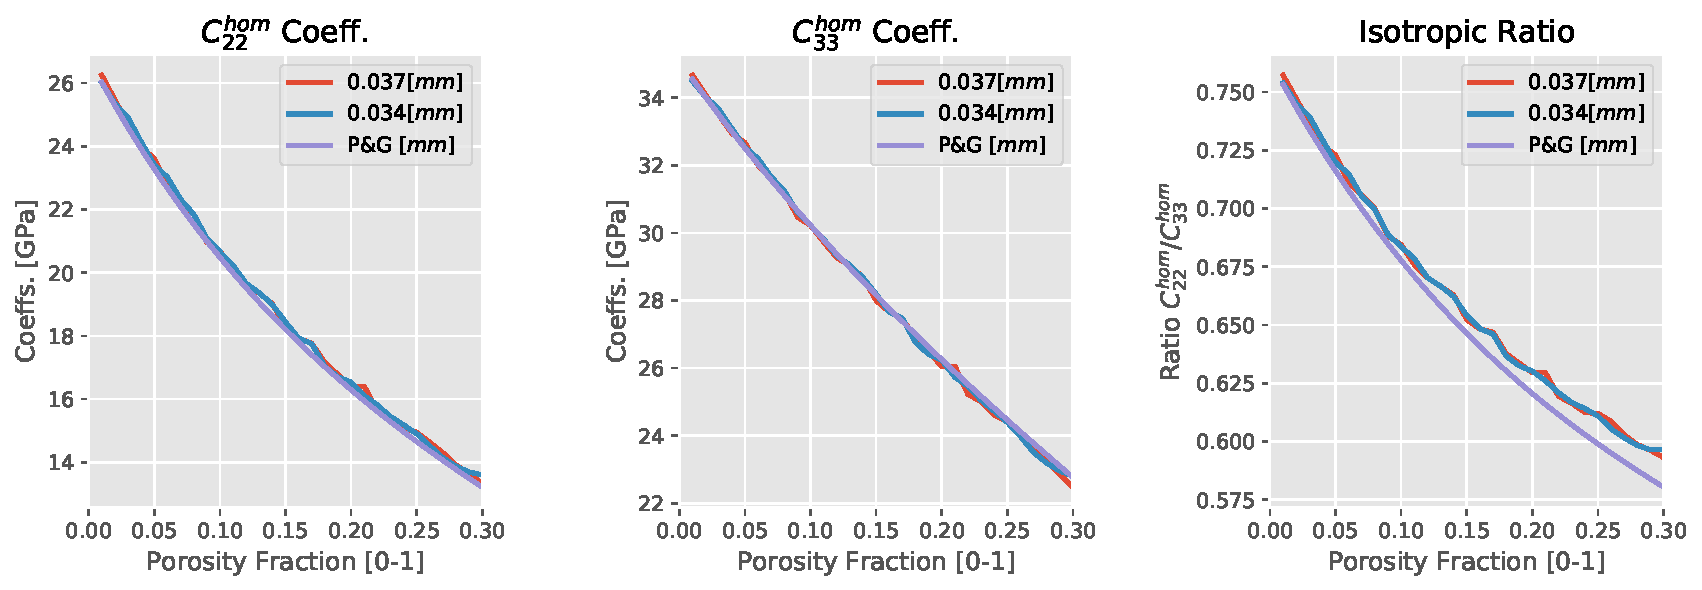
\includegraphics[scale=.5]{images/CellsProb/CellProb_MainHomCoeffsCircular.pdf}
	\caption{Main diagonal elastic homogenized coefficients in \textit{Voigt} notation. They describe an transverse isotropic behavior, spanned in the figure on the biomedical range of $(1,30) [\%]$ cortical porosity. The characteristic microstructure in this case is of unitary square.}
	\label{MainHomCoeffsSquare}
\end{figure}

\begin{figure}[!h]
	\centering
	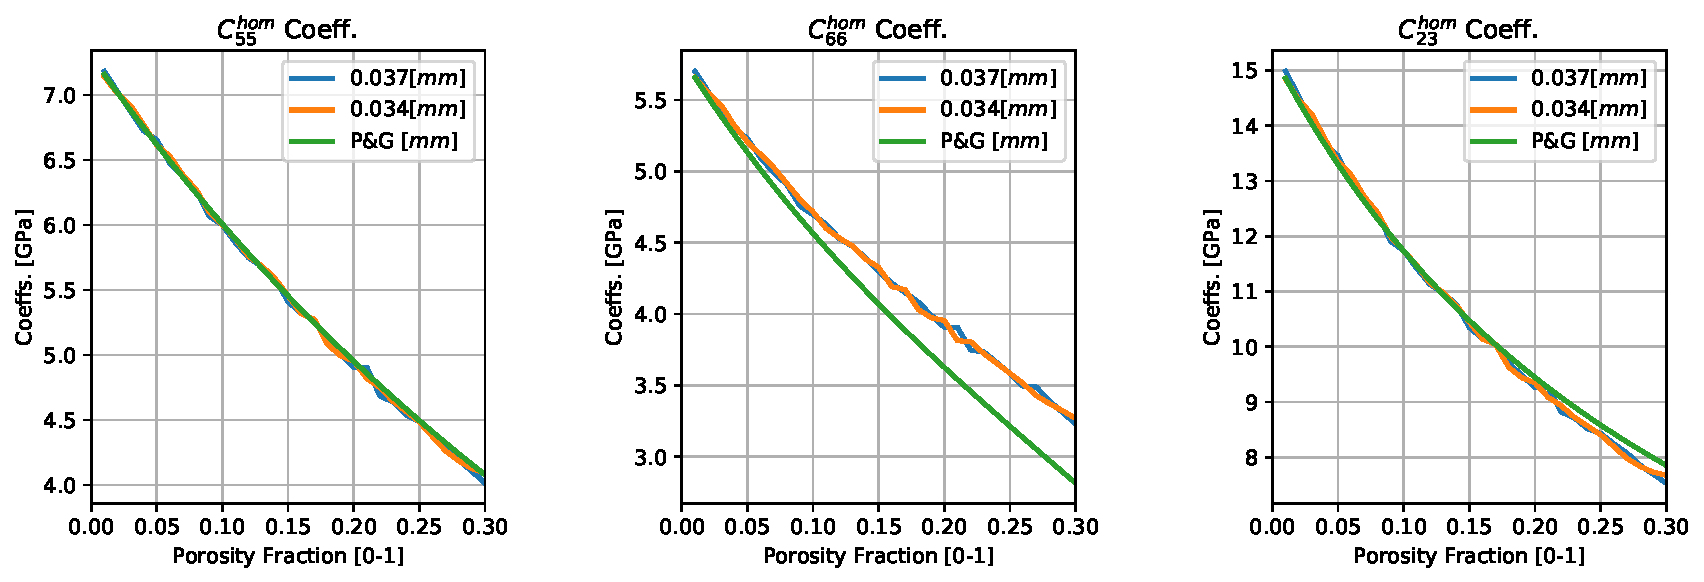
\includegraphics[scale=.5]{images/CellsProb/CellProb_OthersHomCoeffsCircular.pdf}
	\caption{Other diagonal elastic homogenized coefficients in \textit{Voigt} notation. They describe an transverse isotropic behavior, spanned in the figure on the biomedical range of $(1,30) [\%]$ cortical porosity with unitary square characteristic microstructure.}
	\label{OtherHomCoeffsSquare}
\end{figure}

\begin{center}
\begin{tabular}{ |p{2.5cm}||p{2cm}|p{2cm}|p{2cm}|p{2cm}| }
 \hline
 \multicolumn{5}{|c|}{Homogenized Coefficients} \\
 \hline
 Per. Error & $\phi = 5 \%$ & $\phi = 10 \%$ & $\phi = 15 \%$ & $\phi = 20 \%$ \\
 \hline
 $C^{hom}_{22}$ & 0.6 \% & 1.3 \% & 1.3 \% & 1.5 \% \\
 $C^{hom}_{33}$ & 0.1 \% & 0.1 \% & 0.1 \% & 0.1 \% \\
 $C^{hom}_{55}$ & 0.1 \% & 0.1 \% & 0.1 \% & 0.1 \% \\
 $C^{hom}_{66}$ & 1.4 \& & 3.3 \% & 6.3 \% & 9.0 \% \\
 $C^{hom}_{12}$ & 0.8 \% & 1.5 \% & 3.3 \% & 5.9 \% \\
 $C^{hom}_{23}$ & 0.4 \& & 0.1 \% & 0.3 \% & 1.0 \% \\
 \hline
\end{tabular}
\end{center}

\begin{rem}
It's important to note also the periodic microstructure idealization being used in \cite{Parnell2008} since it corresponds to an hexagonal structure defining the mesoscale, while the idealization proposed here is a square microstructure.
\end{rem}

Nevertheless, if we consider now a model using a microstructure as the one defined in \cite{Parnell2008}, i.e., as an hexagonal model with inclusions for the porosity level, the following results are obtained.

\begin{figure}[!h]
	\centering
	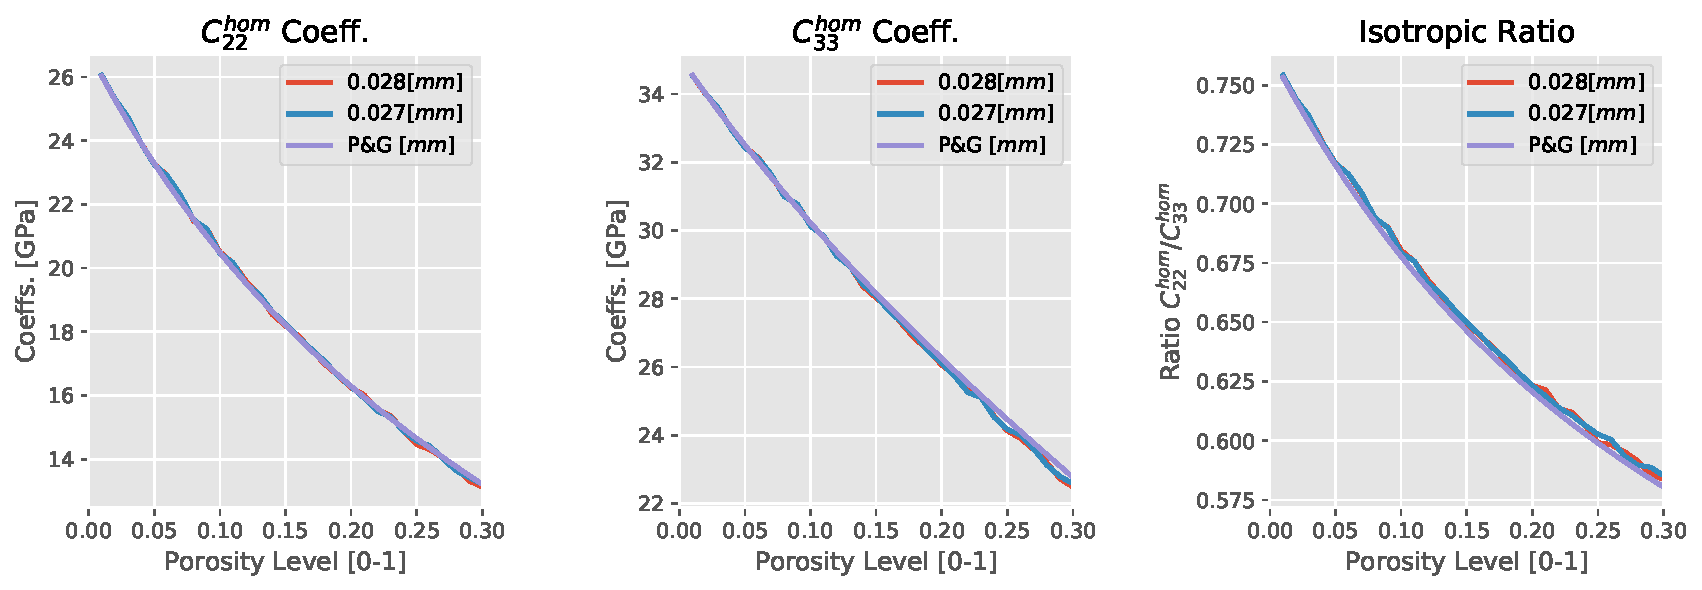
\includegraphics[scale=.5]{images/CellsProb/CellProb_MainHomCoeffsCircularHexa.pdf}
	\caption{Main diagonal elastic tensor coefficients in \textit{Voigt} notation. The figure shows the prediction values over the range $(1,30) [\%]$ of porosity with characteristic microstructure defined by an hexagonal 2-dimensional polygon.}
	\label{MainHomCoeffsHexagonal}
\end{figure}

\begin{figure}[!h]
	\centering
	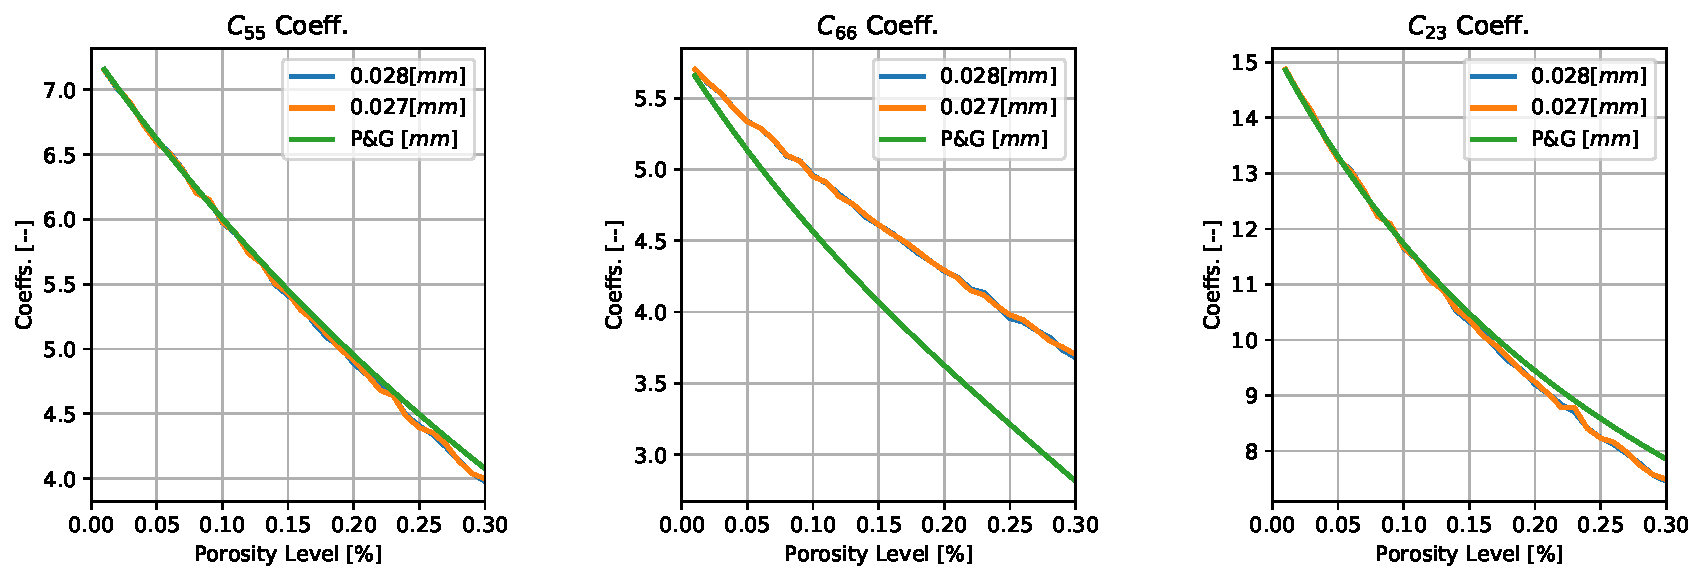
\includegraphics[scale=.5]{images/CellsProb/CellProb_OthersHomCoeffsCircularHexa.pdf}
	\caption{Shear type elastic homogenized coeffs. in \textit{Voigt} notation. The figure shows the behavior over the range $(1,30) [\%]$ porosity with characteristic microstructure described by a hexagonal 2-dimensional polygon.}
	\label{OtherHomCoeffsHexagonal}
\end{figure}

\subsection{Simulations of Wave Propagation}

The simulation setting associated to the experimental measurements is defined by a 2-dimensional rectangular array imitating the frontal plane associated to the cortical bone. The transducer excitation source is defined at the upper surface where the omit the interaction between the human skin and the bone structure itself. 
The experimental measurement procedure consist in the following steps:
\begin{itemize}
    \item Each source associated to the emission transductor is placed approximately at a distance of $0.5 \, [mm]$ from one another, being together a set of 8-12 different sources. 
    \item The detection is obtained by placing approximately from 24-72 sensors depending on the configuration used, where each one is placed at a distance approximately of $0.4 \, [mm]$ from one another.
\end{itemize}
Explicitly, the force acting is modeled in vertical direction associated to the horizontal plane of the skin pointing to the center of the cortical bone with a central time $t_0 > 0$ and oscillation speed $\tau_0 > 0$, i.e., described in the form:
\begin{equation}
    \mathbf{F}(\mathbf{x},t) = - e^{\frac{(t-t_0)^2}{2\sigma^2}} cos( 2 \pi t \tau_0 ) \mathbb{I}_{\mathbf{x} \in \Gamma_i} \hat{j} \quad \text{ on } \Gamma_N
\end{equation}
where $\{ \Gamma_i\}_{ i \in \{1,\dots, 8\}} \subset \Gamma_N$ denotes a disjoint subset of boundaries where the force is applied. 
Over such kind of configuration it can be proved theoretically the existence of the so-called \textit{Lamb}-waves that describe the particular propagation of guided waves associated to the elastic coefficients and density of the model being used.
In particular, the presence of a closed domain implies reflection with different directions related to the \textit{Neumann} or \textit{Dirichlet} respectively.

\subsubsection{Case of Multiple Sources}
Its simulated under the setting of 8 force sources positioned at equal distances of one to another. It defines then 8 different experiment thus wave-guided propagation with its recordings.
The figure \ref{FK-DiagramS8P12M10} describes the \textit{Lamb}-waves curves with the numerically simulated $(f,k)$-diagram. It shows the validation of the numerical model with respect to the theoretical prediction curves, observing clear correspondence between symmetrical and anti-symmetrical modes.

\begin{figure}[!h]
	\centering
	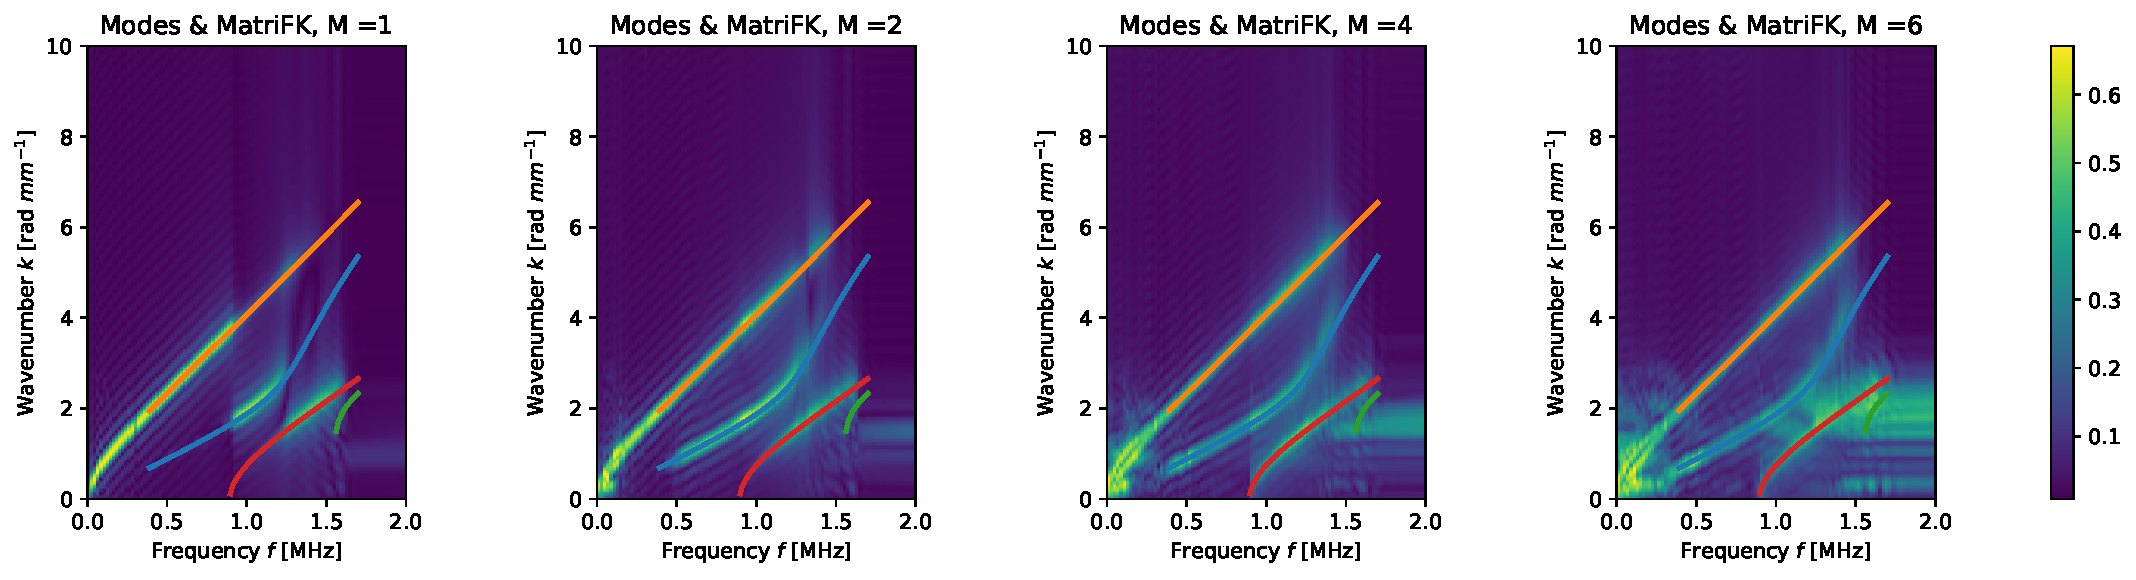
\includegraphics[width=\textwidth]{images/TimeMultSous/2DTimeS8P12ElasticFK10M780_y.pdf}
	\caption{Numerically Simulated $(f,k)$-diagram of 2D Transverse Elastodynamic Model: Setting of 8 sources with $12\%$ porosity and thickness of $1.0 [mm]$.}
	\label{FK-DiagramS8P12M10}
\end{figure}

Similarly \ref{SVD-S8P12M10} describes the modes in $[dB]$ from the singular value decomposition of the recording array. It shows the preponderance of the first three modes describing the wave-front.

\begin{figure}[!h]
	\centering
	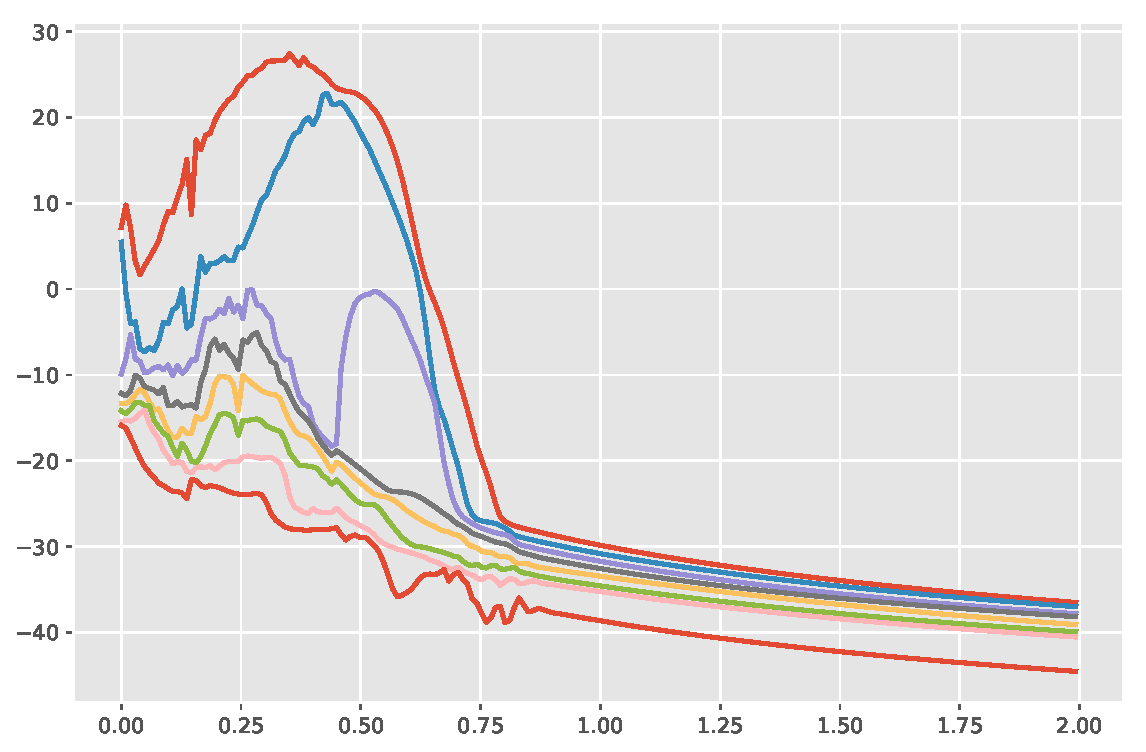
\includegraphics[scale=.5]{images/TimeMultSous/2DTimeS8P12Elastic10_SV.pdf}
	\caption{Singular values obtained by the SVD decomposition of the recorded signal from the simulation \ref{FK-DiagramS8P12M10}}
	\label{SVD-S8P12M10}
\end{figure}

The presence of several symmetric and antisymmetric modes expressed by the \textit{Lamb} waves is related experimentally with higher thickness values, since in this case the range of horizontal propagation is bigger.
Under such consideration, its shown on figure \ref{FK-DiagramS8P3M28} the wave-front simulations for a different pair $(Th., Po.)$, displaying a greater number of prediction curves.

\begin{figure}[!h]
	\centering
	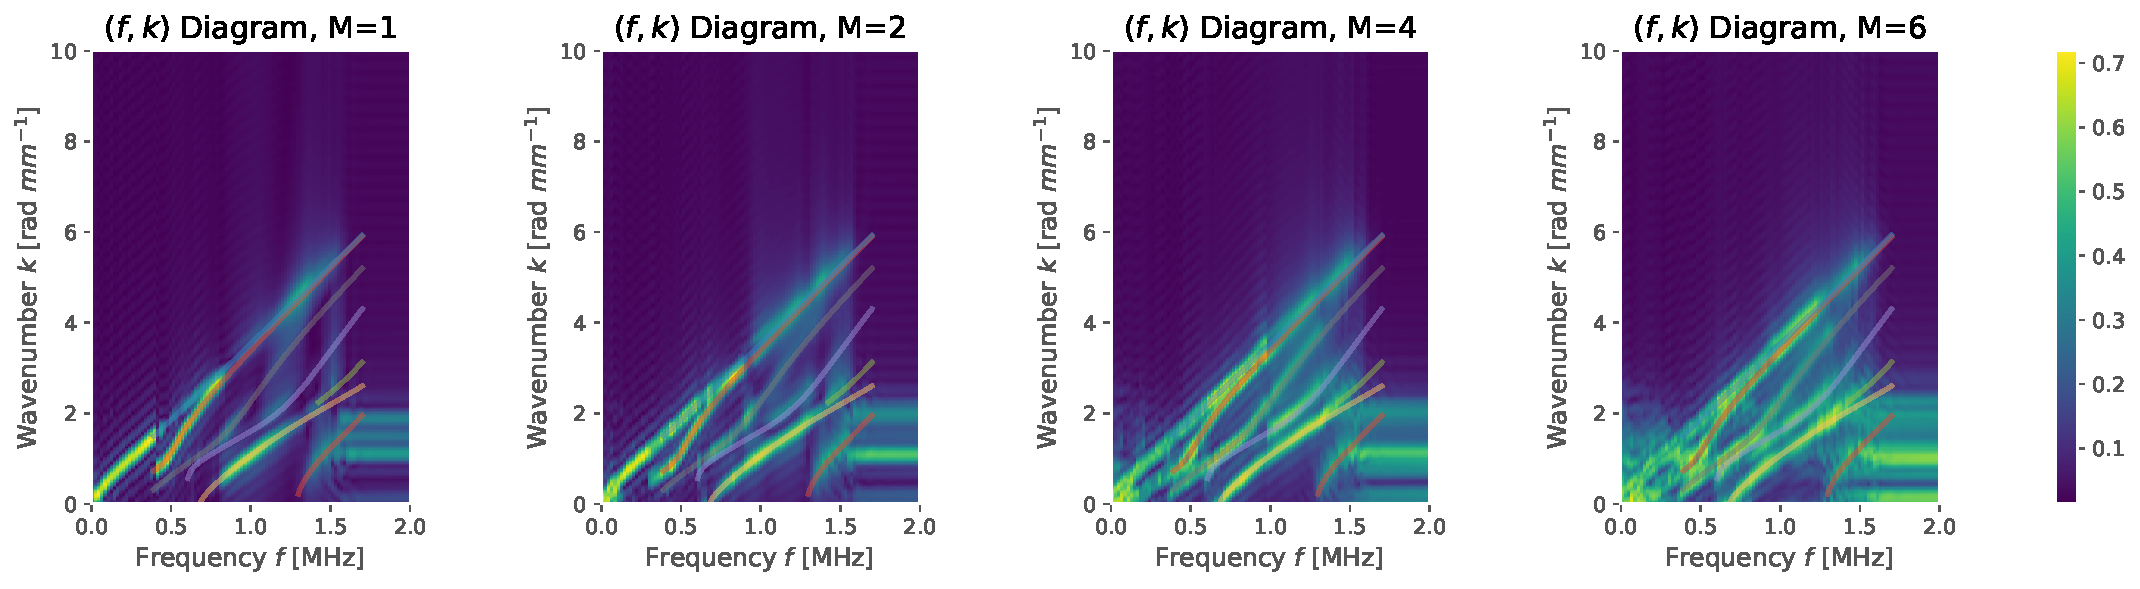
\includegraphics[width=\textwidth]{images/TimeMultSous/2DTimeS8P3ElasticFK28M780_y.pdf}
	\caption{Numerically Simulated $(f,k)$-diagram of 2D Transverse Elastodynamic Model: Setting of 8 sources with $3\%$ porosity and thickness of $2.8 [mm]$.}
	\label{FK-DiagramS8P3M28}
\end{figure}

Similarly, the corresponding modes in $[dB]$ from the singular value decomposition of the recording signal is shown on \ref{SVD-S8P3M28}, that compares naturally to the experimental reference literature.

\begin{figure}[!h]
	\centering
	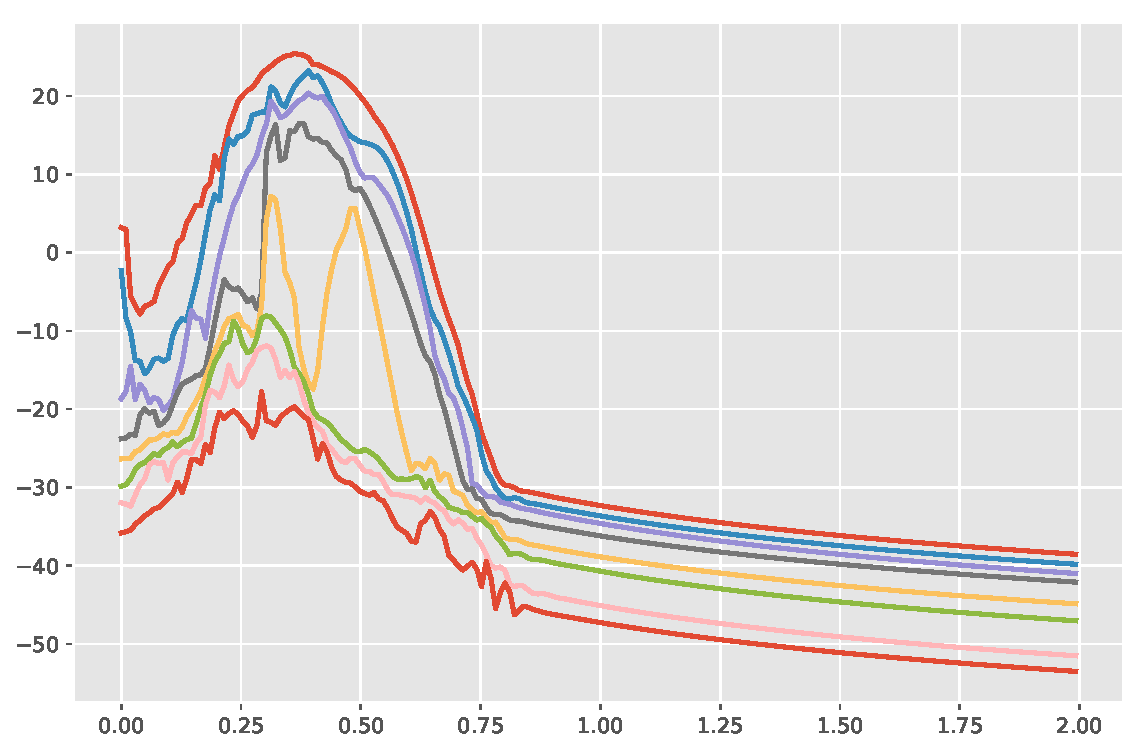
\includegraphics[scale=.5]{images/TimeMultSous/2DTimeS8P3Elastic28_SV.pdf}
	\caption{Singular values obtained by the SVD decomposition of the recorded signal from the simulation \ref{FK-DiagramS8P3M28}}
	\label{SVD-S8P3M28}
\end{figure}



\subsubsection{Case of a Single Source}
The above study of 8-source simulations to generate one sample of data introduces the problems of computational simulation under limited resources and time. 
To tackle such problem, its used the space invariance of the elastic wave since the recording to generate the output data array corresponds to just a space translation of the input signal for each one of the 8 propagation, thus such setting can be exchanged for one source with a higher number of sensors lowering the time-cost of the full simulation to 1/8 of the initial time.

Its shown then on figure \ref{FK-DiagramS1P6M33} the $(f,k)$-diagram associated to the 1-source simulations setting. It presents natural reflections related to the rectangular 2-dimensional domain used with mixed boundary conditions.
\begin{figure}[!h]
	\centering
	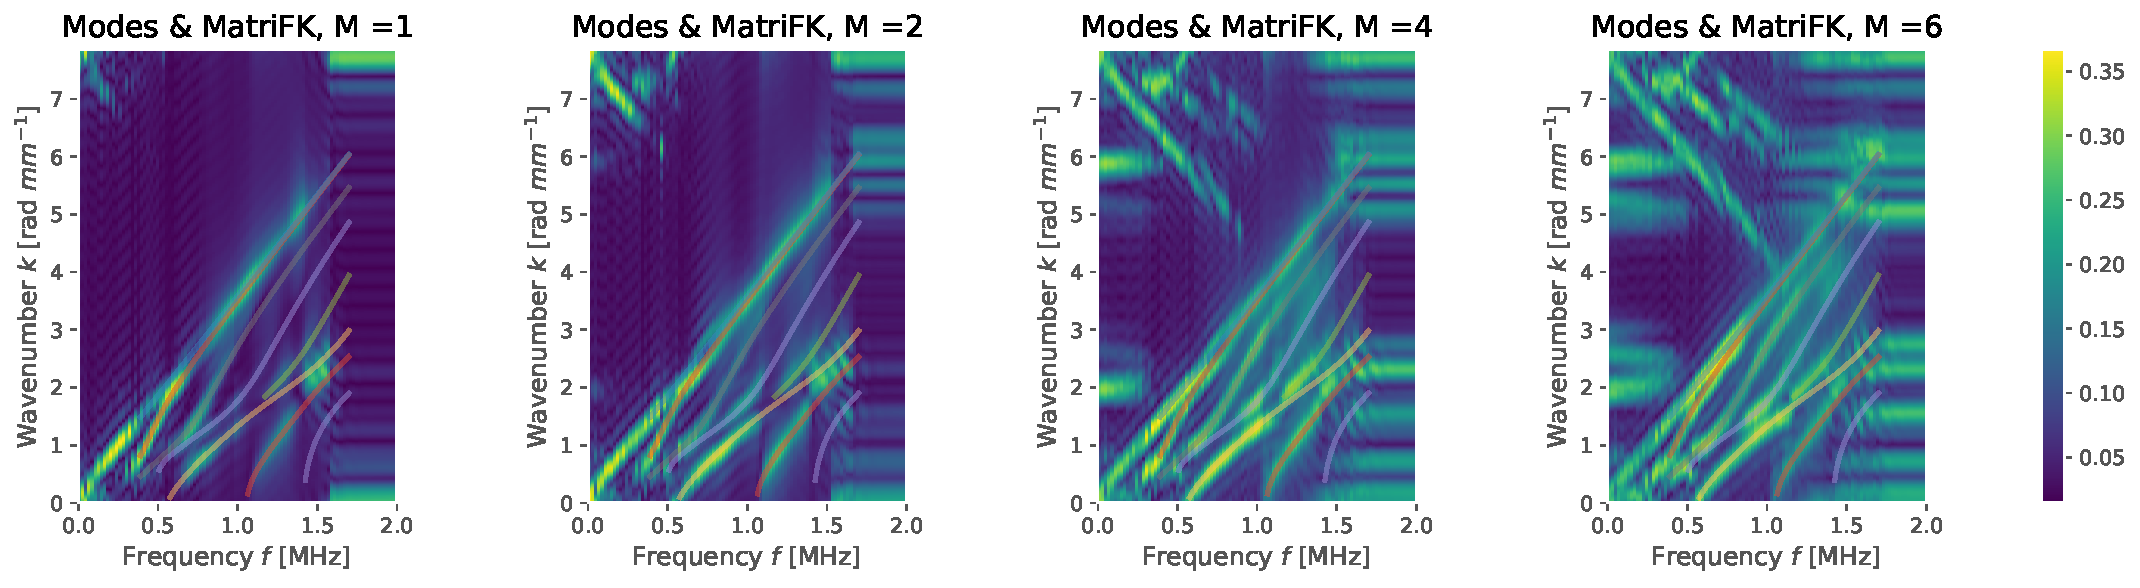
\includegraphics[width=\textwidth]{images/TimeSingSous/2DTime_P6ElasticFK33M1460_y.pdf}
	\caption{Numerically Simulated $(f,k)$-diagram of 2D Transverse Elastodynamic Model: Setting of 1 source with $6\%$ porosity and thickness of $3.3 [mm]$.}
	\label{FK-DiagramS1P6M33}
\end{figure}

Its shown moreover on figure \ref{SVD-S1P6M33} the main modes $[dB]$ associated to the recorded signal.
\begin{figure}[!h]
	\centering
	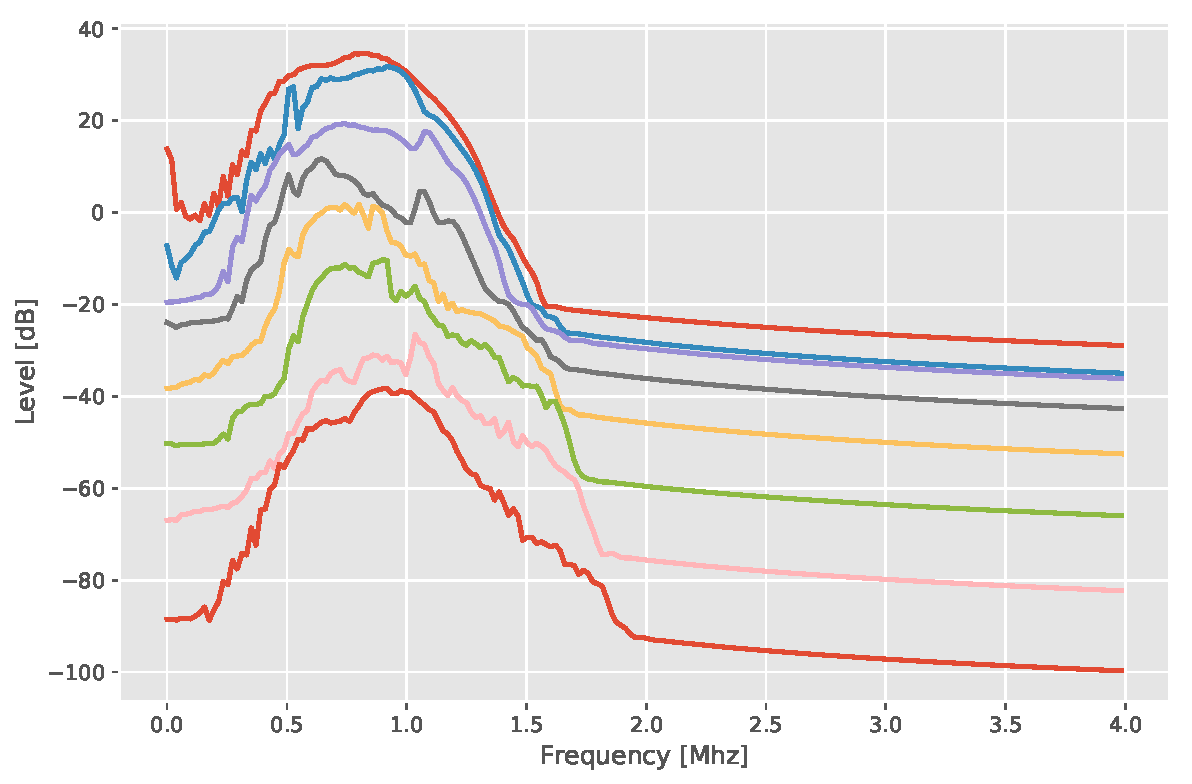
\includegraphics[scale=.5]{images/TimeSingSous/2DTime_P6Elastic33_SV.pdf}
	\caption{Singular values obtained by the SVD decomposition of the recorded signal from the simulation \ref{FK-DiagramS1P6M33}}
	\label{SVD-S1P6M33}
\end{figure}

The reflections shown in the image above produced from the simulations corresponds to an aliasing effect in the input signal $S(f_n, e_m, \mathbf{x}_p)_{(m,p) \in [N^E]\times [N^R]}$ after applying FFT over the space $[N^E] \times [N^R]$. Such aliasing express the folding of the $k$-variable \footnote{Associated to the wavenumber} by the conjugation property on \texttt{FFT}, i.e., 
\begin{equation*}
    \overline{\texttt{FFT}(S(f_n, \cdot, e_m))(k)} := \sum_{m=0}^M S(f_n, \mathbf{x}_p, e_m) \overline{e^{-2 \pi i \frac{p k}{M}}} = \texttt{FFT}(S(f_n, \cdot, e_m))(-k)
\end{equation*}
in such a way that the norm associated is the same. Moreover since we consider a finite wavenumber interval denoted $[0, k_{max}]$, such a reflected wavenumber is given by $k_{max}-k$ as observed in the figure.

Given such a symmetry, its considered the application of the analytic projector defined for a given signal $s$ regular enough by:
\begin{equation*}
    \mathcal{P}(s) := (I + \mathbf{i}\mathcal{H})(s)
\end{equation*}
being $\mathcal{H}$ the Hilbert transform. Such a projector defines the analytic signal of $s$ by constructing its real and imaginary parts.

Since the behavior observed in the $(f,k)$-diagrams are of symmetry, a natural idea is to use the \textit{Hilbert} transform on the input signal, obtaining a analytic signal which maintains the structure of the \textit{Lamb} modes and moreover recreates experimentally obtained results \textit{in-vivo} and \textit{ex-vivo}.
Applying then such a projection filter we obtain the results qualitatively and quantitatively similar with respect to the real experimental data.

\begin{figure}[!h]
	\centering
	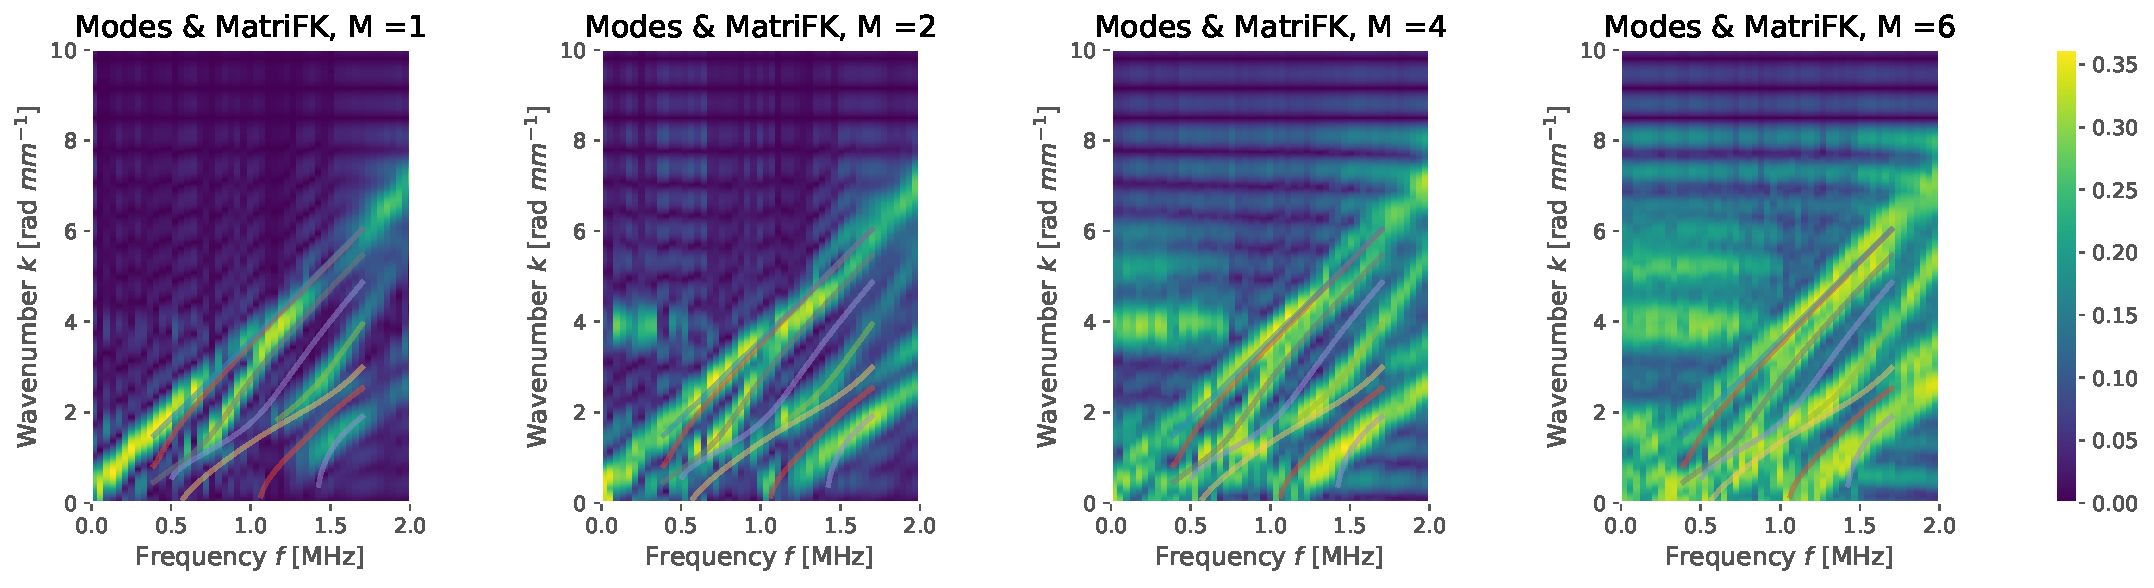
\includegraphics[width=\textwidth]{images/TimeSingSous/2DTimeHilb_P6ElasticFK33M1460_y.pdf}
	\caption{Numerically Simulated $(f,k)$-diagram of 2D Elastodynamic Model: Setting of 1 source with $6\%$ porosity and thickness of $3.3 [mm]$ appplying Hilbert transform to delete reflexions.}
	\label{FK-Hil-DiagramS1P6M33}
\end{figure} 

\begin{figure}[!h]  
	\centering
	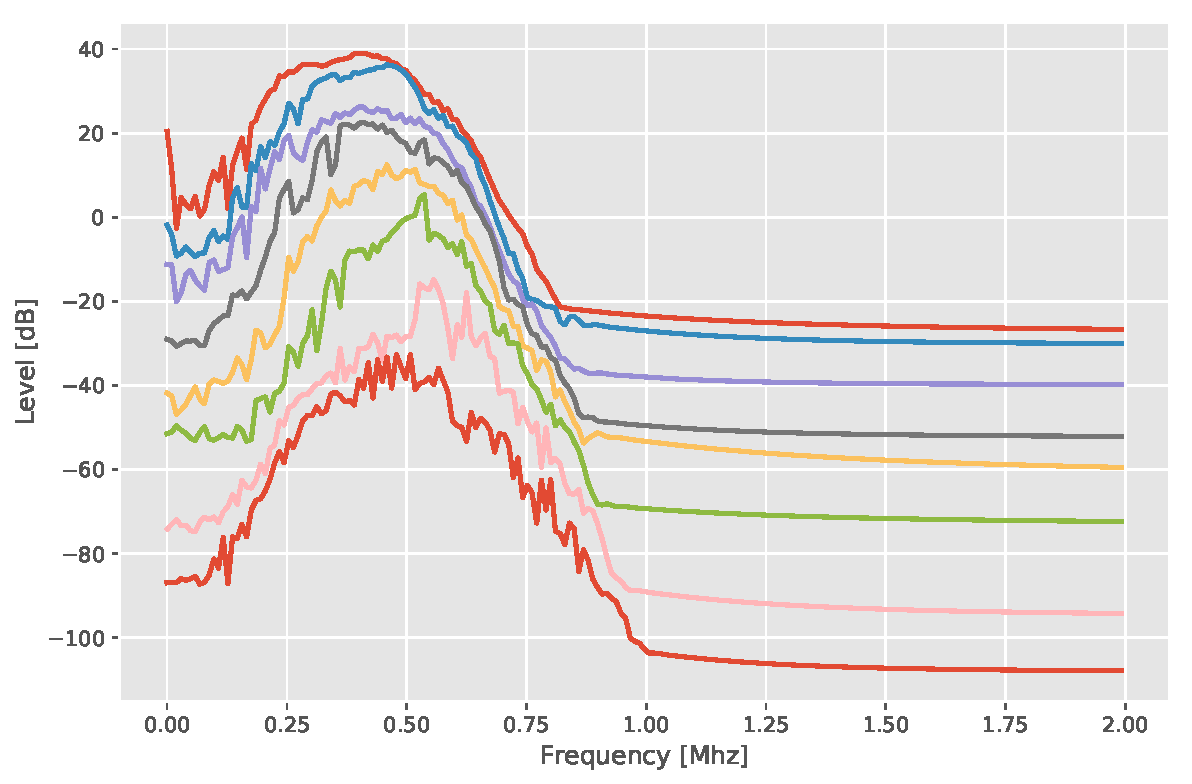
\includegraphics[scale=.5]{images/TimeSingSous/2DTimeHilb_P6Elastic33_SV.pdf}
	\caption{Singular values obtained by the SVD decomposition of the recorded signal from the simulation \ref{FK-Hil-DiagramS1P6M33}}
	\label{SVD-Hil-S1P7M33}
\end{figure}

\subsection{Case on Frequency Domain}

The time-domain simulation given results which represent qualitatively the model with enough fidelity, nevertheless such simulation requires a relatively small time step in such a way that the full simulation take considerable time. Thus, it is necessary to consider a model which reduces the computational cost.
To this end, taking into account that the signal processing involves the application of \texttt{FFT} over the sensors data, a straightforward method is to consider the simulations now in the time-domain over the arrays of frequencies that are of interest.

\subsubsection{Solutions without Attenuation}
In this case, using the schemes proposed in the section before showed results in which Lamb-Waves and also $dB$ figures where affected by distortions FIGURE BELOW. Such kind of behavior repeated over different pairs of porosity level and thickness associated to the simulations, in such a way that was necessary to study the spectrum of the elastic operator.

\begin{figure}[!h]
	\centering
	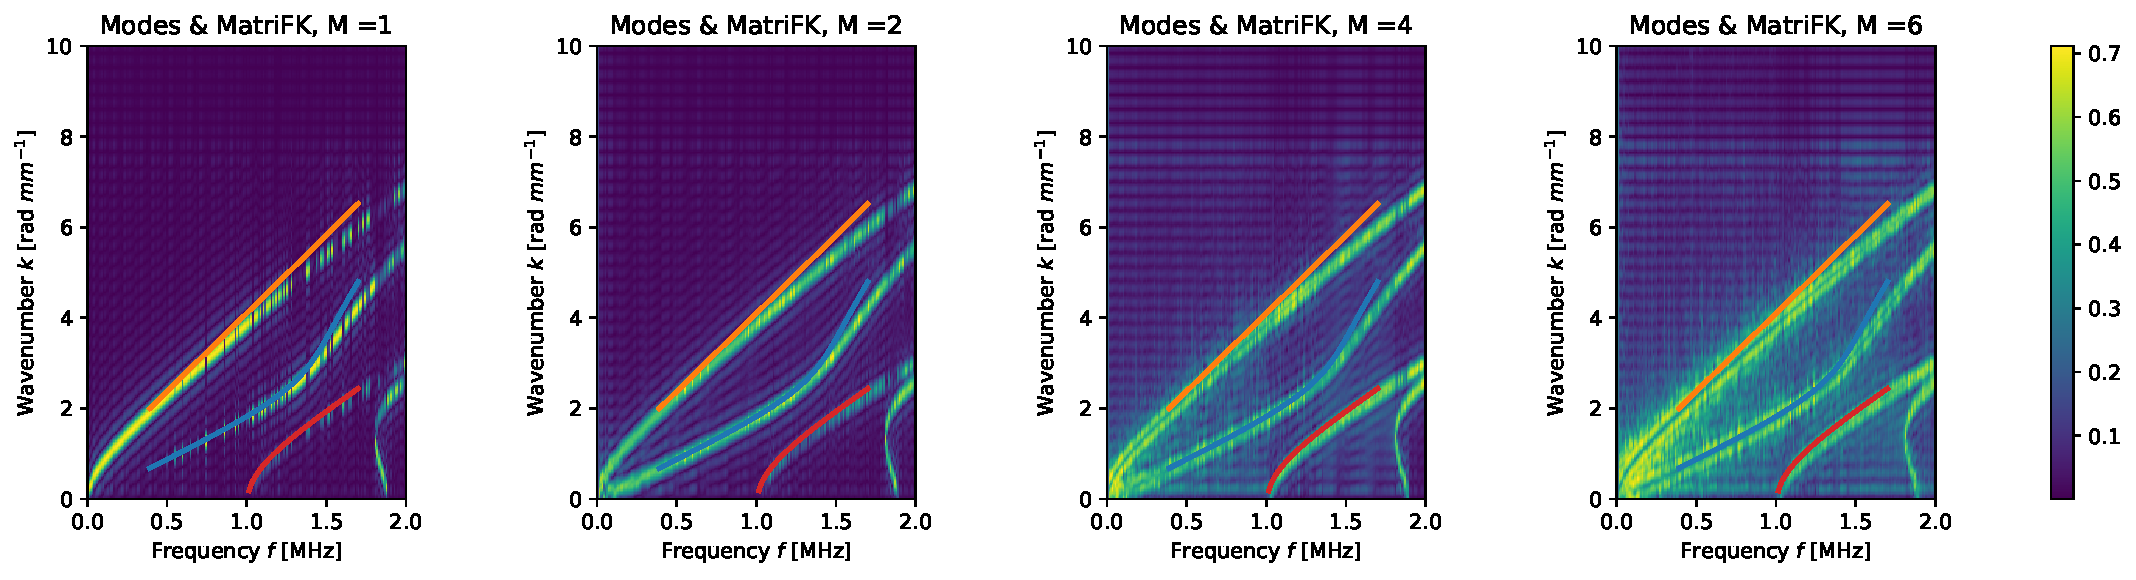
\includegraphics[width=\textwidth]{images/FreqRes/2DFreqS8P10ElasticFK09M300_y.pdf}
	\caption{Numerically Simulated $(f,k)$-diagram of 2D Elastic Model on Frequency Domain: Setting of 8 sources with $10\%$ porosity and thickness of $0.9 [mm]$}
	\label{FK-Freq-DiagramS8P10M09}
\end{figure} 

\begin{figure}[!h]
	\centering
	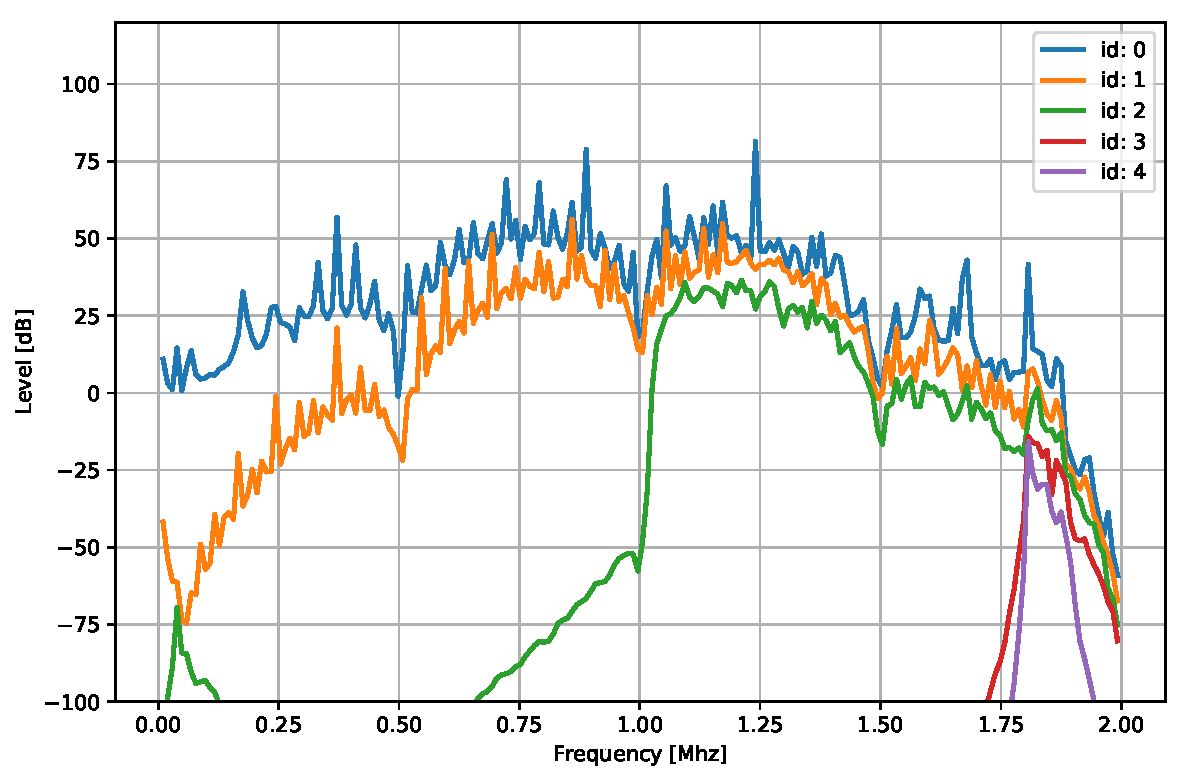
\includegraphics[scale=.5]{images/FreqRes/2DFreqS810Elastic09_SV.pdf}
	\caption{Singular values obtained by the SVD decomposition of the recorded signal from the simulation \ref{FK-Freq-DiagramS8P10M09}}
	\label{SVD-Freq-S8P10M09}
\end{figure} 

Such a study corresponds to the formulation of an eigenvalue problem associated to the elastic operator, defined as finding the pairs $\{(\lambda_k, u_k) \, : \, k \in \mathbb{N} \} \subset \mathbb{R}_+ \times \mathbf{H}^1(\Omega, \Gamma_D)$ solution to the following variational form:

\begin{equation*}
    \label{VariationalEigenProb}
    \mathcal{I}_{\mathbf{C}^{hom}} (u_k, v) = \lambda_k (u_k, v)_{\Omega} \quad \forall v \in \mathbf{H}^1(\Omega, \Gamma_D)
\end{equation*}
where we identify each eigenvalue to the eigenfrequency associated to our problem in the form:
\begin{equation*}
    \lambda_k = \rho^0 (2\pi f_k)^2, \text{ i.e. } f_k = \frac{1}{2\pi} \sqrt{\frac{\lambda_k}{\rho^0}} \quad k \in \mathbb{N}_{*}
\end{equation*}

\begin{rem}
Ket us note in particular that the existence of such pairs is obtained from a classical result of elliptic theory \cite{raviart1983introduction}, \cite{evans2010partial}. Explicitly, it follows since the homogenized coefficients are elliptic and moreover they are bounded which gives us a well-defined bilinear, bicontinuous and coercive operator $\mathcal{I}_{\mathbf{C}^{hom}}(\cdot, \cdot)$ and a linear continuous operator $b(\cdot) := (u_k, \cdot)$ defined respectively on $\mathbf{H}^1(\Omega, \Gamma_D)^2$ and $\mathbf{H}^1(\Omega, \Gamma_D)$.
\end{rem}



It was found numerically a spectrum with abundant eigen-frequencies in bounded intervals of frequency (predicted from the theory), nevertheless the experimental frequency array which was necessary to use for further studies in connection with the real data, showed a neighborhood of at least eigen-frequencies over each experimentally selected frequency. 

In (\ref{EigenValuesComparison}) is shown the frequencies used in the experimental setting used for the simulations in the frequency domain and the eigen-frequencies associated to the operator under study.

\begin{figure}%
    \centering
    \subfloat[Start Bandwidth]{{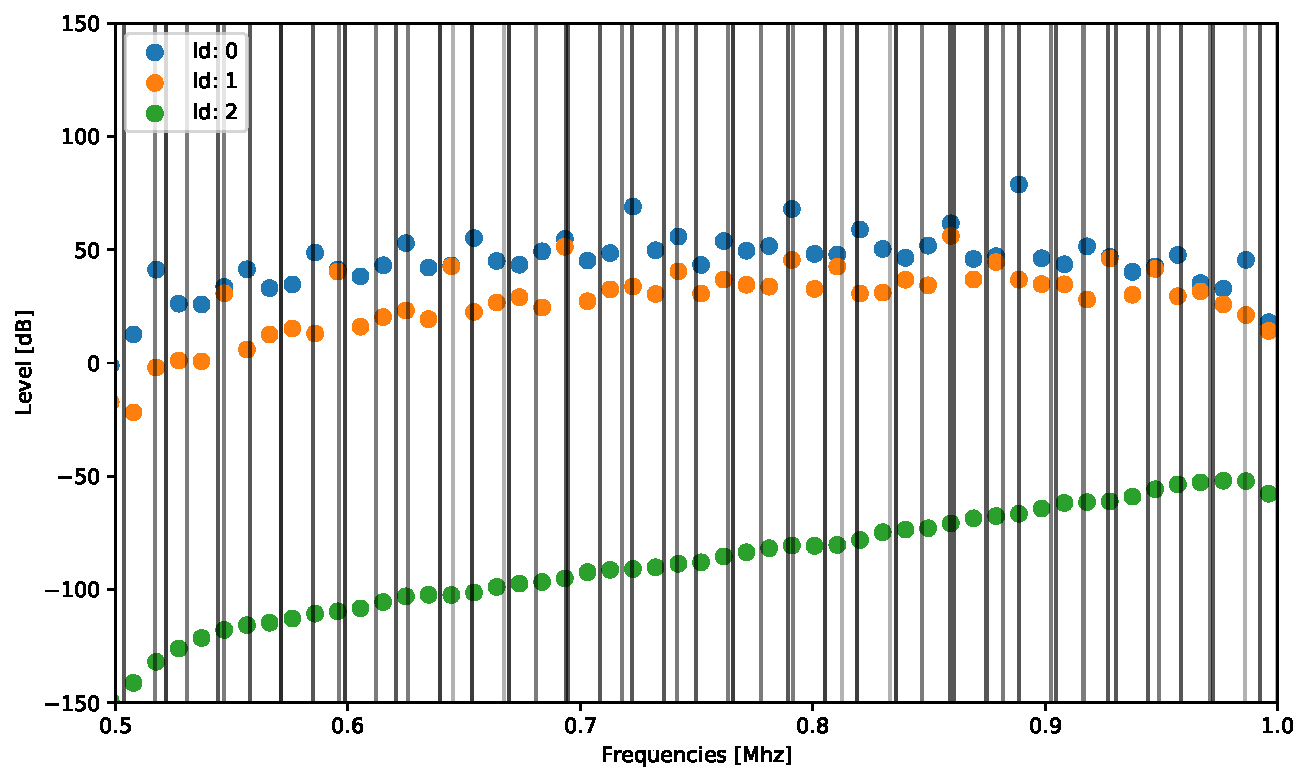
\includegraphics[width=7cm]{images/FreqRes/SingValues-EigenFreqs05-10.pdf} }}%
    \qquad
    \subfloat[End Bandwith]{{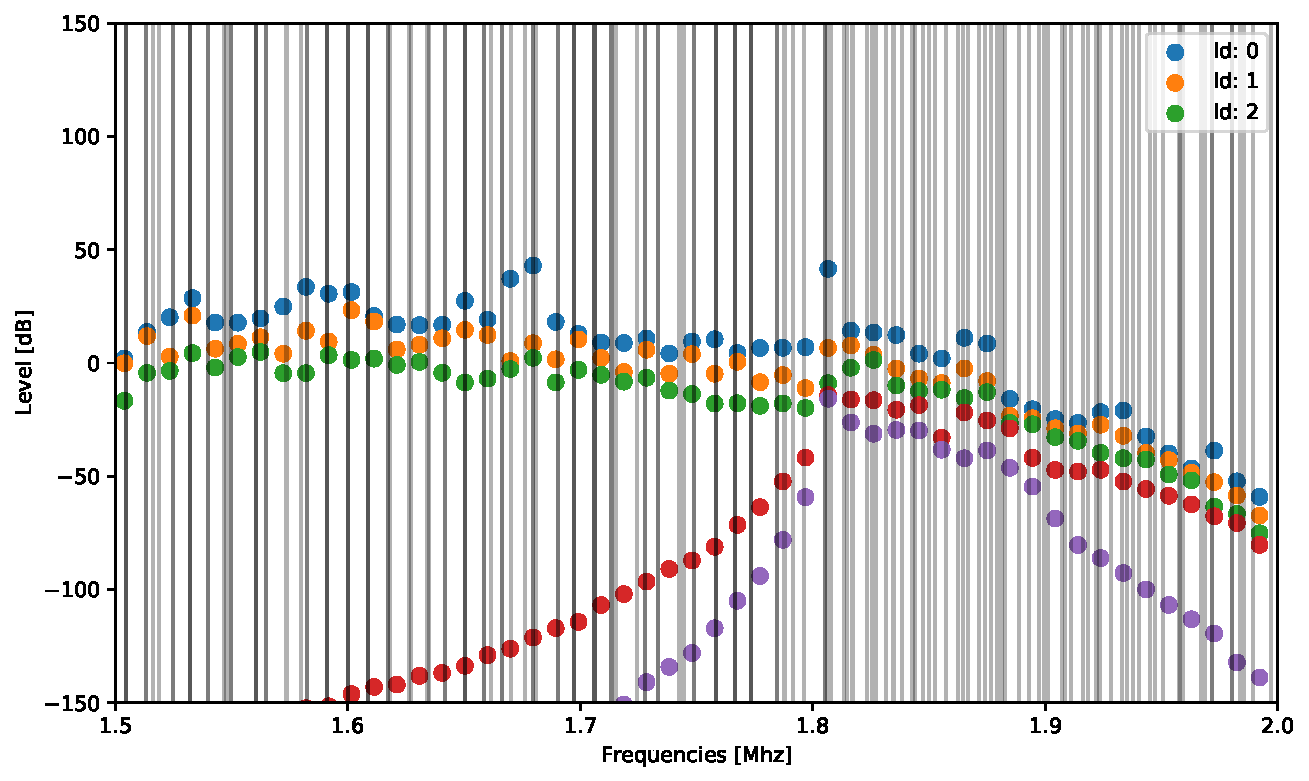
\includegraphics[width=7cm]{images/FreqRes/SingValues-EigenFreqs15-20.pdf} }}%
    \caption{Comparison between Singular Values and Eigen-frequencies: Experimentally its found a increasing sequence of eigenvalues that intersects the experimentally chosen array frequencies.}%
    \label{EigenValuesComparison}%
\end{figure}


\subsubsection{Solution using Attenuation.}
To fix the oscillation observed in the frequency-domain problem we consider adding a $\epsilon$ viscous-like term, such model in particular defines a translation of the eigenfrequencies from the elastic operator to the complex plane thus avoiding the real plane resonances. This implies moreover that we are avoiding the ill-conditioned matrix system from the FEM space discretization.

Fixing a frequency $\omega \in \mathbb{R}$, let us consider solutions in the form: $u(\mathbf{x},t) = e^{2 \pi i \omega t}\hat{u}(\mathbf{x})$, so that $\hat{u}(\mathbf{x})$ solves the equivalent problem in the frequency domain
\begin{equation*}
    \left \{
    \begin{array}{ccc}
        -(2\pi \omega)^2 \rho^0 \hat{u}(\mathbf{x}) - i \epsilon \hat{u}(\mathbf{x}) - \nabla \cdot \sigma(\hat{u}) = \mathbf{0} & \text{ in } \Omega \times [0,T] \\
        \hat{u} = \mathbf{0} & \text{ on } \Gamma_D\\
        \sigma(\hat{u}) \cdot n = \mathbf{F}(\mathbf{x}, \omega) & \text{ on }\Gamma_N \times [0,T]
    \end{array}
    \right .
\end{equation*}
Taking into account that the current \texttt{FEniCS} version doesn't support the usage of a complex coefficient formulation in the variational form, we decompose the solution in its real and complex part as $\hat{u} = \hat{u}_R + i \hat{u}_I$. It follow then the coupled system satisfied for the pair $(\hat{u}_R, \hat{u}_I)$ given by:
\begin{equation*}
    \left \{
    \begin{array}{cc}
        -(2\pi \omega)^2 \rho^0 \hat{u}_R +  \omega \epsilon \hat{u}_I - \nabla \cdot \sigma (\hat{u}_R) = \mathbf{0} & \text{ in }\Omega \times [0,T] \\
        -(2\pi \omega)^2 \rho^0 \hat{u}_I - \omega \epsilon \hat{u}_R - \nabla \cdot \sigma (\hat{u}_I) = \mathbf{0} & \text{ in }\Omega \times [0, T] \\
        \hat{u}_R, \hat{u}_I = \mathbf{0} & \text{ on } \Gamma_D \\
        \sigma(\hat{u}_R)\cdot n, \sigma(\hat{u}_I)\cdot n = \hat{\mathbf{F}}_R, \hat{\mathbf{F}}_I & \text{ on }\Gamma_N
    \end{array}
    \right.
\end{equation*}
which can be solved with the standard tools of \texttt{FEniCS} by the usage of a mixed element for the couple system.

Its shown then on figure \ref{FK-DiagramFreqS8P12M28} the $(f,k)$-diagram associated to the 8-sources simulations setting. It presents natural reflections related to the rectangular 2-dimensional domain used with mixed boundary conditions.
\begin{figure}[!h]
	\centering
	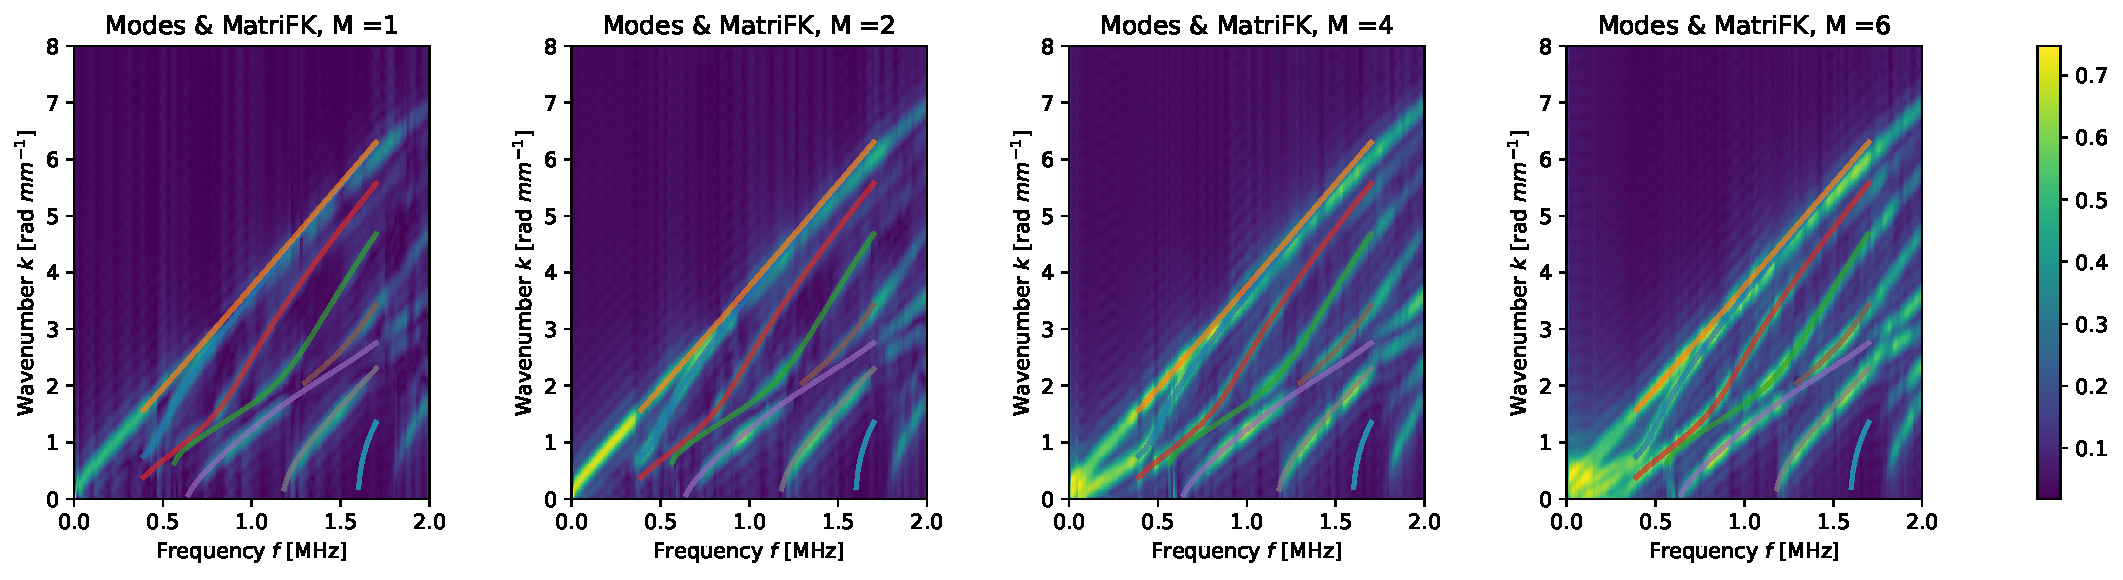
\includegraphics[width=\textwidth]{images/FreqMultSous/2DMixedP12TransIsoFKW28M400_y.pdf}
	\caption{Numerically Simulated $(f,k)$-diagram of 2D Transverse Elastodynamic Model: Setting of 1 source with $3\%$ porosity and thickness of $3.0 [mm]$.}
	\label{FK-DiagramFreqS8P12M28}
\end{figure}

Nevertheless, from the figure \ref{SVD-S1P7M30} of main modes $[dB]$ associated to the recorded signal, its observed vanishing oscillation of the modes, thus numerically avoiding the eigenfrequencies, the main resonance cause.
\begin{figure}[!h]
	\centering
	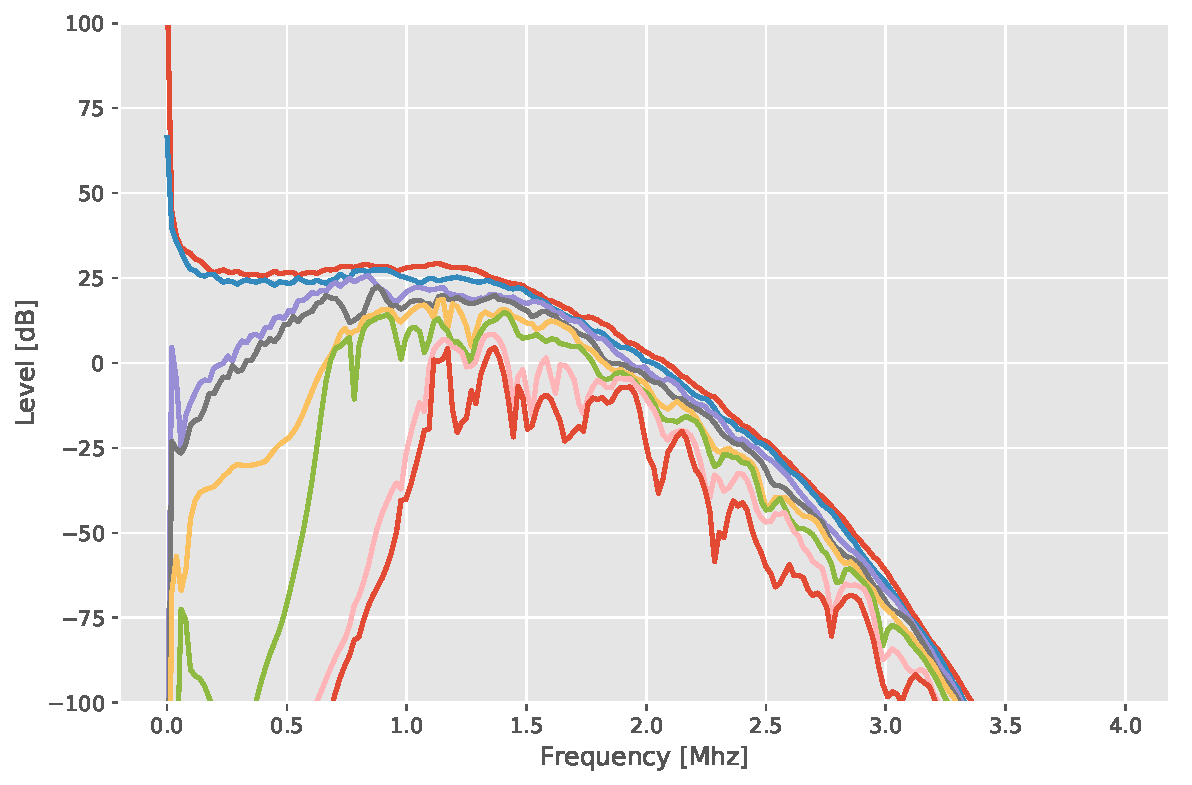
\includegraphics[scale=.5]{images/FreqMultSous/2D-FreqSimP12W28eKV_SV.pdf}
	\caption{Singular values obtained by the SVD decomposition of the recorded signal from the simulation \ref{FK-DiagramFreqS8P12M28}}
	\label{SVD-FreqS8P12M28}
\end{figure}


\subsection{Simulation of Wave Propagation on 3-dimension}
Following the 2-dimensional case, its now studied the effect of radial wave behavior on the recorded signal, validating in particular the experimentally obtained results that neglect the non-axial wave-guide propagation. 
Such procedures imply the creation of adaptive meshes to the complex cortical bone geometry, where open-source software such as \texttt{iso2mesh}, \texttt{CGAL} is used for its generation and in particular a created a pipeline of mesh generation from $\mu$-CT images.

\subsubsection{Half-Cylinder Case}
A half-cylinder mesh is proposed as first approximation to the 3-dimensional real cortical bone sample from the $\mu$-CT images. In this case, avoiding the non-uniformity characteristic of the bone surface, its tested the waveguide propagation and distortion generated by the natural curvature of the mesh.


\subsubsection{Rugous Exterior}
The mesh generation is done, using the following pipeline dataflow:

\begin{figure}[!h]
	\centering
	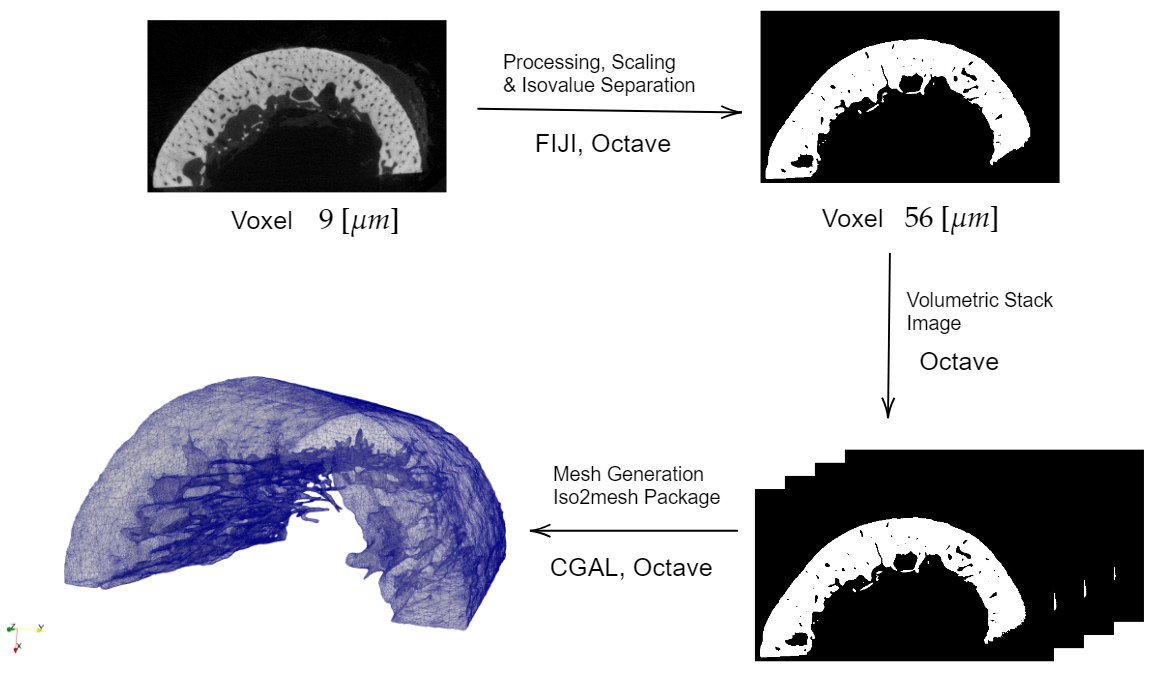
\includegraphics[scale=.5]{images/ImgExt/DiagramMeshGeneration.png}
	\caption{Pipeline: The mesh generation involves a sequence of different softwares that generates the desired domain where the simulations takes place.}
	\label{DiagramMeshGeneration}
\end{figure} 

\subsubsection{Fully Porous Material}
The save Pipeline (\ref{DiagramMeshGeneration}) is used for the mesh generation, now without homogenized coefficients and therefore taking into account the variation on the elastic coefficients depending on the presence of mesoscale structure and cavities.

\chapter{Predictions}
\section{Viscoelasticity}
%The ultrasound method \cite{Foiret2014} enables the simultaneous measurement of cortical thickness and tissue elastic properties where previous techniques such as DXA (the \textit{de facto} method) could archieve.
As studied before, factors of risk fracture are the thickness, porosity and particular quality elements of the extracelular matrix as explained in \cite{Bernard2015}. The QUS method \cite{Foiret2014}, \cite{Minonzio2018} of axial transmission technique is based on recording from the propagation of guided waves over the media, were damping factors affect the signal. This is associated to a viscoelastic behavior of the cortical bone arising mainly from the presence of collagen fibers, specifically treated with Resonant Ultrasound Spectroscopy techniques. Thus, its natural to study the correspondence between such damping elements and their preponderance on the resulting homogenized coefficients by the two-scale homogenization theory

\textit{Bernard} \textit{et al. }\cite{Bernard2015} studied in a viscoelastic behavior on a frequency domain model of bone their results, in which he modelled the elastic tensor $C^*_{ij}$ with damping effect given by:
\begin{equation*}
C^*_{ij} = C_{ij} + i C_{ij}^{'} = C_{ij} (1+ iQ_{ij}^{-1})
\end{equation*}

where the $Q^{-1}_{ij}$ are defined as ratios of the imaginary part ($C_{ij}'$) to the real part ($C_{ij}$), denoting the so-called quality factors.

In this section, I shall formulate such quality factors following the two-scale homogenization formalism, recovering the homogenized coefficients in the elastic case at different porosity levels and particularly obtaining prediction for the quality factors at some interval. Under the actual literature, such coefficients are yet to be validated since there isn't enough experimental literature to confirm our predictions.


\section{Formalization of Q-factors}
The idea for this section is to formalize the Q-factor in the framework of homogenized equations.
In this case, we will give a definition for the Q-factor from a elastodynamic Kelvin-Voigt model of bone.\\
More specifically, we define the mechanical behavior of bone as a multiphase viscoelastic material composed of two-phases with cell unit in the form $\mathbf{Y} = Y_{m} \cup Y_{f}$ being the matrix and fluid parts respectively.
For the bone matrix, we associate an elastic behavior defined by the elastic coefficient:
\begin{equation*}
    C_{ijkl}(\mathbf{y}) = C_{ijkl}^m \mathbb{I}_{Y_m}(\mathbf{y}) + C_{ijkl}^f \mathbb{I}_{Y_f}(\mathbf{y})
\end{equation*}
while the bone marrow is defined modelled as the viscous part, associated to a coefficient given in the form:
\begin{equation*}
    D_{ijkl}(\mathbf{y}) =  D_{ijkl}^m \mathbb{I}_{Y_m}(\mathbf{y}) + D_{ijkl}^f \mathbb{I}_{Y_f}(\mathbf{y})
\end{equation*}
Moreover, the relations between both coefficients is given as an attenuation specified by parameters $\epsilon^{(m)}, \epsilon^{(f)} >0$ associated to the bone matrix and marrow respectively. Explicitely, we assume then:
\begin{equation*}
    D_{ijkl}^m(\mathbf{y}) = \epsilon^{(m)} C_{ijkl}^m(\mathbf{y}) , \quad D_{ijkl}^f (\mathbf{y}) = \epsilon^{(f)} C_{ijkl}^f(\mathbf{y})
\end{equation*}


\begin{rem}
By fixing this kind of relation, the idea is to obtain a model of viscoelasticity in which the viscous part can be modelled by a linear attenuation of the elastic one, so that the overall behavior is transverse isotropic defined with just a pair of parameters $(\epsilon^m, \epsilon^w)$ that mimic closely the experimental behavior of bone.
\end{rem}

\subsection{Workflow}
\begin{rem}
For the case of 2D modelling of transverse isotropic material, the simulated solutions are close enough to \textit{Parnel and Grimal} prediction with their approximation method.
\end{rem}
In time domain, we consider an elastodynamic model of Kelvin-Voigt type behavior with mixed boundary conditions, described in the form:
\begin{equation*}
    \left \{
    \begin{array}{cc}
        \rho^{\epsilon}\partial_{tt}u - \nabla \cdot \sigma(u, \partial_t u) = \mathbf{0} & \text{ in } (0,T)\times \Omega \\
        \sigma^{\epsilon}(u,\partial_t u)  = \mathbf{C}:\mathbf{e}(u) + \mathbf{D}:\mathbf{e}(\partial_t u) & \text{ in } (0,T)\times\Omega \\
        \sigma^{\epsilon}(u, \partial_t u)\cdot n = \mathbf{F} & \text{ on }(0,T)\times \Gamma_N \\ 
        u = \mathbf{0} & \text{ on } (0,T)\times \Gamma_D
    \end{array}
    \right .
\end{equation*}
\begin{rem}
In the above and the next developments, we assume resting initial conditions, i.e., $\partial_t u = u = \mathbf{0}$, not written explicitly in the models and deduction.
\end{rem}
Using now the fourier transform defined at frequency $\omega \in \mathbb{R}$ with base $\{e^{i\omega t}\}_{\omega}$, we obtain our redefined problem in the Fourier domain given by:
\begin{equation*}
    \left \{
    \begin{array}{cc}
        -\omega^2 \rho^{\epsilon} \hat{u}^{\epsilon} - \nabla \cdot \hat{\sigma}_{\epsilon,\omega}(\hat{u}^{\epsilon}) = \mathbf{0} & \text{ in } \Omega  \\
        \hat{\sigma}_{\epsilon,\omega} (\hat{u}^{\epsilon}) = (\mathbf{C} + i\omega \mathbf{D}):\mathbf{e}(\hat{u}^{\epsilon}) & \text{ in } \Omega \\
        \hat{\sigma}_{\epsilon,\omega} (\hat{u}^{\epsilon}) \cdot n = \hat{\mathbf{F}}(\omega) & \text{ on } \Gamma_N \\
        \hat{u}^{\epsilon} = \mathbf{0} & \text{ on } \Gamma_D
    \end{array}
    \right .
\end{equation*}
such that at $\omega = 0$ we have $\hat{u}^{\epsilon}=\mathbf{0}$ at $\Omega$.\\

Now, homogenizing by using the two-scale asymptotic method, it follows for effective (macroscopic) model defined at frequency $\omega$ by:
\begin{equation*}
    \left \{
    \begin{array}{cc}
        -\omega^2 \rho^{0} \hat{u}^0 - \nabla \cdot \hat{\sigma}^0(\hat{u}^0)  = \mathbf{0} & \text{ in } \Omega \\
        \hat{\sigma}^{0} (\hat{u}^0)  = (\mathbf{C} + i\omega \mathbf{D})^{hom}:\mathbf{e}(\hat{u}^0) & \text{ in } \Omega \\
        \hat{\sigma}^{0} (\hat{u}^0) \cdot n = \hat{\mathbf{F}}(\omega) & \text{ on } \Gamma_N \\
        \hat{u}^0 = \mathbf{0} & \text{ on } \Gamma_D
    \end{array}
    \right .
\end{equation*}

In particular, the homogenized coefficients, are defined by the cell problem solutions $N^{rs} \in \mathbf{H}^1_{\#}(\mathbf{Y}, \mathbb{C})$, described for each $r,s \in \{1,2,3\}$ in the form
\begin{equation*}
    \left \{
    \begin{array}{cc}
         \partial_{y_j} \big[ \big( C_{ijkl} + i\omega D_{ijkl} \big) \mathbf{e}_{kl}(N^{rs}) \big] &= - \partial_{y_j} \big[ C_{ijkl} + i\omega D_{ijkl} \big] \quad \forall y \in \mathbf{Y} \\
        \big \langle C_{ijkl} + p D_{ijkl} \big \rangle_{\mathbf{Y}}  = 0 & 
    \end{array}
    \right.
\end{equation*}
\begin{rem}
Since the cell problems must be valid for each $\omega \in \mathbb{R}$ and for each $\mathbf{y} \in \mathbf{Y}$ we would like to decouple the cell PDE problems so that we can define a ratio viscosity-elasticity, i.e. an expression for the Q-factor.
\end{rem}
The decoupling is then defined by considering the separation between the real and imaginary parts associated to the cell solutions, i.e., by considering the decomposition
\begin{equation*}
    N^{rs}(\mathbf{y}) = \mathbf{N}_R^{rs}(\mathbf{y}) + i\mathbf{N}_I^{rs}(\mathbf{y})
\end{equation*}
being now the vectors functions $\mathbf{N}_R^{rs}, \mathbf{N}_I^{rs}$ in $\mathbf{H}^1_{\#}(\mathbf{Y},\mathbb{R})$ solving the following PDE system associated to the real and imaginary part decomposition:
\begin{equation*}
    \left \{
    \begin{array}{cc}
        \partial_{y_j} \big[ C_{ijkl} \mathbf{e}_{kl}(\mathbf{N}^{rs}_R) -\omega D_{ijkl} \mathbf{e}_{kl}(\mathbf{N}^{rs}_I) \big] = - \partial_{y_j} \big[ C_{ijrs} \big] & \forall \mathbf{y} \in \mathbf{Y} \\
        \partial_{y_j} \big[ C_{ijkl} \mathbf{e}_{kl}(\mathbf{N}^{rs}_I) +\omega D_{ijkl} \mathbf{e}_{kl}(\mathbf{N}^{rs}_R) \big] = - \partial_{y_j} \big[ \omega D_{ijrs} \big] & \forall \mathbf{y} \in \mathbf{Y} \\
        \big \langle \mathbf{N}^{rs}_R \big \rangle_{\mathbf{Y}},\big \langle \mathbf{N}^{rs}_I \big \rangle_{\mathbf{Y}} = \mathbf{0}  &
    \end{array}
    \right.
\end{equation*}
\begin{rem}
Note in particular that for the above cell problems, we existence and uniqueness of a weak solution is guaranteed since the problem can be rewritten as a fully elliptic operator, being the solution unique by applying the normalization condition on mean equal $\mathbf{0}$.
\end{rem}
With the solution to the cell problem, we can then define the homogenized coefficients associated to the elastic and viscous part by recalling first:
\begin{equation*}
    \hat{\sigma}_{ij}^0 (\hat{u}^0,\omega) = R_{ijkl}^{hom} (\omega) \mathbf{e}_{kl}(\hat{u}^0)
\end{equation*}
being the homogenized tensor
\begin{equation*}
    R^{hom}_{ijrs}= \big \langle  C_{ijrs} + i\omega D_{ijrs} + \big( C_{ijkl} + i \omega D_{ijkl} \mathbf{e}_{kl}(\mathbf{N}^{rs}) \big) \big \rangle  
\end{equation*}
so that, using the decomposition of $N^{rs}$ it follows that:
\begin{align*}
    R^{hom}_{ijrs} &= \big \langle C_{ijrs} + \big( C_{ijkl}\mathbf{e}_{kl}( \mathbf{N}^{rs}_R) -\omega D_{ijkl}\mathbf{e}_{kl}(\mathbf{N}^{rs}_I) \big) \big \rangle \\
    & \, + i \big \langle \omega D_{ijrs} + \big( C_{ijkl} \mathbf{e}_{kl}(\mathbf{N}^{rs}_I) + \omega D_{ijkl}\mathbf{e}_{kl}(\mathbf{N}^{rs}_R) \big) \big \rangle \\
    & := C^{hom}_{ijrs} + \mathbf{i} \omega D^{hom}_{ijrs}
\end{align*}

It follows in particular, the definition of the $Q_{ij}$ factor, defined directly on the tensor coefficients is given by:
\begin{equation}
    \label{Qfactor-Def}
    Q_{ijrs}^{-1}(\omega) := \frac{D^{hom}_{ijrs}(\omega)}{ C^{hom}_{ijrs}(\omega)}
\end{equation}
where the homogenized coefficients are defined as above.
Let us note the preponderant dependency of the frequency associated on the defined factor, which as study above, derives explicitly from the Kelvin-Voigt viscoelastic assumption of the mechanical model. 

An aspect that must be taken into account is the nonlinear effect produced added from the asymtotic asumption on the solution, expressed in the term $N^{rs}$ at the homogenized coefficients definition that can be explicitly stated from (\ref{Qfactor-Def}).
Its possible to account for that effect by taking a decomposition on the linear part associated to the mean over the coefficient itself and the nonlinear effect produced from the solutions to the cell problems, i.e., from (\ref{Qfactor-Def}) the decomposition in its linear and nonlinear effects its obtained as:
\begin{equation}
    \label{Expansion-Qfactor}
    \begin{aligned}
        Q_{ijrs}^{-1}  & = \frac{D_{hom}^{(0)} + D_{hom}^{(1)}}{C_{hom}^{(0)} + C_{hom}^{(1)}}  \\
         & =  \frac{D_{hom}^{(0)}}{C_{hom}^{(0)}} + \frac{1}{C^{(0)}_{hom}( C^{(0)}_{hom} + C^{(1)}_{hom}} \big[C^{(0)}_{hom} \big( D^{(0)}_{hom} + D^{(1)}_{hom}\big) - D^{(0)}\big( C^{(0)}_{hom} + C^{(1)}_{hom} \big) \big]
    \end{aligned}
\end{equation}
where its being used the notation for the linear terms in $p \in [0,1]$ (porosity) by:
\begin{equation*}
    C^{(0)}_{hom} = \langle C_{ijrs} \rangle_{\mathbf{Y}} \quad  D^{(0)}_{hom} = \langle D_{ijrs} \rangle_{\mathbf{Y}}
\end{equation*}
and the nonlinear terms with respect to $p \in [0,1]$ associated to the solutions $N^{rs}$ given by:
\begin{equation*}
    \begin{array}{cc}
        C^{(1)}_{hom} =& \langle C_{ijkl}\mathbf{e}_{kl}(N^{rs}_R) - \omega D_{ijkl}\mathbf{e}_{kl}(N^{rs}_I) \rangle_{\mathbf{Y}} \\
        D^{(1)}_{hom} =& \langle \omega^{-1} C_{ijkl}\mathbf{e}_{kl}(N^{rs}_I) + D_{ijkl}\mathbf{e}_{kl}(N^{rs}_R) \rangle_{\mathbf{Y}} 
    \end{array}
\end{equation*}

\subsection{Predictions}

PREDICTIONS WITH RESPECT TO BERNARD PAPER
VARIATIONS USING DIFFERENT EPSILON VALUE.

INDEPENDENCE WITH RESPECT TO THE FREQUENCY.
\begin{figure}[!h]
	\centering
	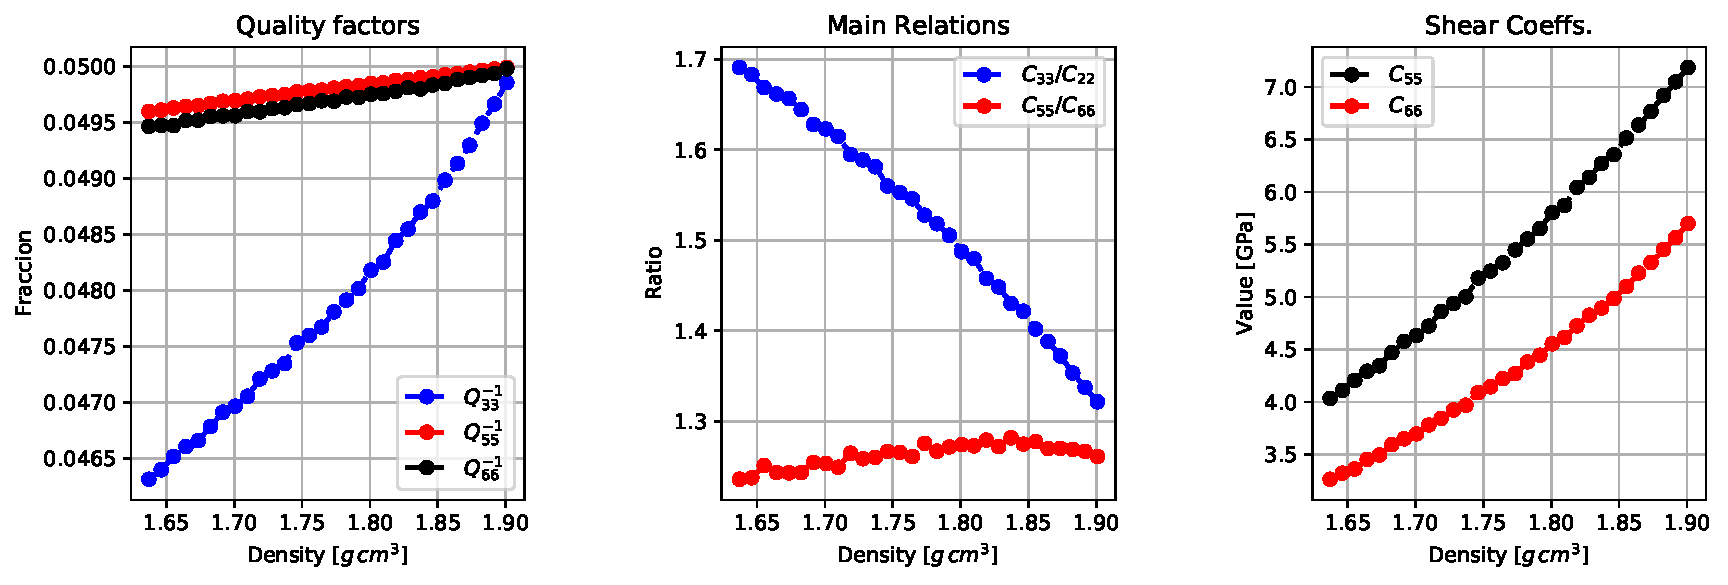
\includegraphics[width=\textwidth]{images/Qfactors/CellProb_QfactorCircular5E-2_Relations.pdf}
	\caption{Predicted Behavior for the Viscoelastic Model: Its shown on the left figure the predicted quality factors for a \textit{Kelvin-Voigt} model; the center figure a prediction of homogenized coefficient ratios, and on the right figure some homogenized shear ratios behaves as in \cite{Bernard2015} }
	\label{PredictionHomCoeffs-Qfactor}
\end{figure} 
\begin{figure}[!h]
	\centering
	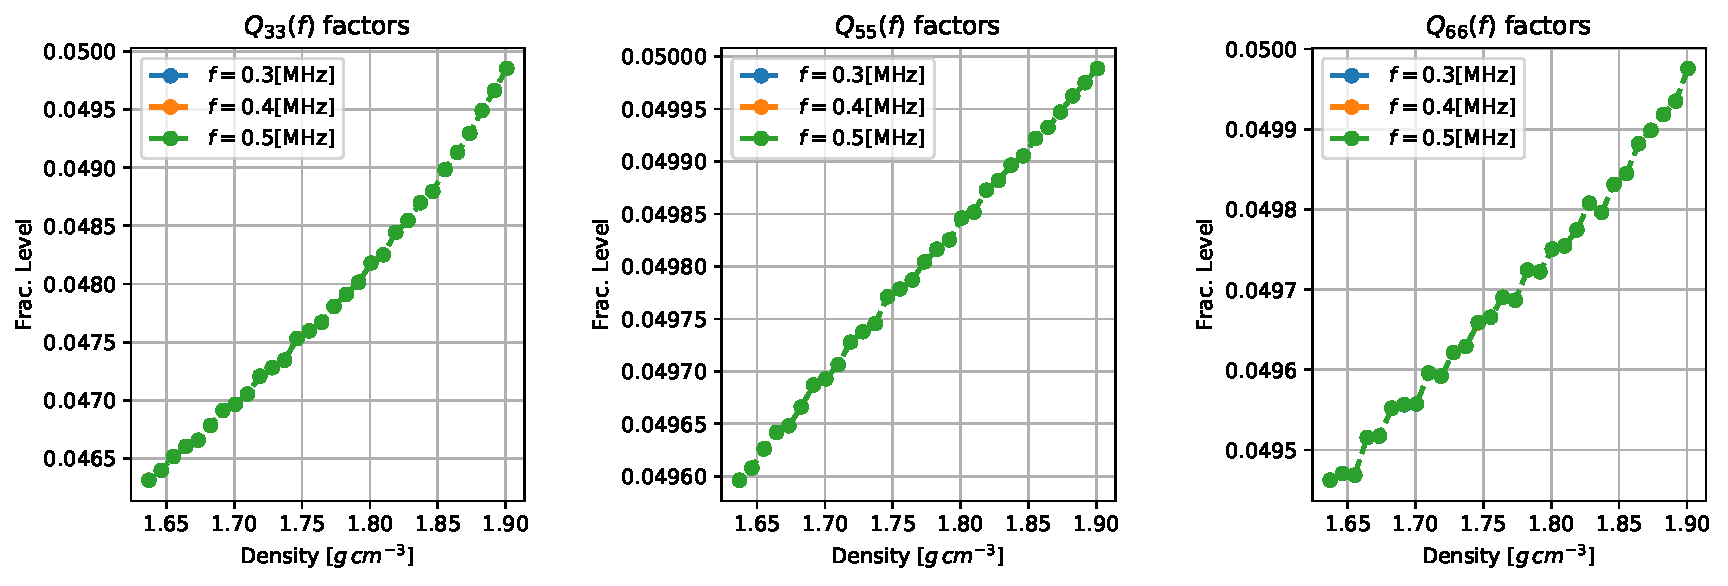
\includegraphics[width=\textwidth]{images/Qfactors/QfactorsFreqsEPS5-2.pdf}
	\caption{Predicted Behavior for the Viscoelastic Model: Its shown on the left figure the predicted quality factors for a \textit{Kelvin-Voigt} model; the center figure a prediction of homogenized coefficient ratios, and on the right figure some homogenized shear ratios behaves as in \cite{Bernard2015} }
	\label{PredictionHomCoeffs-Qfactor}
\end{figure} 





\begin{conclusion}
	\lipsum[130-132]
	\begin{figure}[!h]
		\centering
		
\includegraphics[scale=.2]{images/fcfm.pdf}
		\caption{Logo de la Facultad}
		\label{logofcfm}
	\end{figure}
	\lipsum[133-134]
	\begin{table}[!h]
		\centering
		\begin{tabular}{|c||c|}
			\hline
			Campo 1& Campo 2\\\hline
			Valor 1& Valor2\\\hline
		\end{tabular}
		\caption{Tabla 1}
		\label{tabla:1}
	\end{table}
	\lipsum[135]
\end{conclusion}


% \input{glosario.tex} % optional

\bibliographystyle{plain} 
\bibliography{bibliography}

% \input{anexo_apendices.tex} % optional

\end{document}
